\documentclass[a4paper,10pt,twoside]{StyleThese}

\def\myauthor{Hugues Van Assel}
\def\mytitle{Phd Thesis}


\synctex=1
\setlength{\marginparwidth}{2cm}
\usepackage[left=3cm,right=3cm,top=2.5cm,bottom=2.5cm,includefoot,includehead,headheight=13.6pt]{geometry}

\renewcommand{\baselinestretch}{1.05}
\renewcommand{\baselinestretch}{1.05}

\newcommand{\refname}{{\sffamily References}}
\usepackage{aecompl}
\usepackage[intoc]{nomencl}
\renewcommand{\nomname}{Notations and Acronyms}
\nomlabelwidth=25mm
\makenomenclature
\renewcommand{\nomgroup}[1]{\ifthenelse{\equal{#1}{N}}{\item[\Large\sffamily\textbf{Notations}]}{\ifthenelse{\equal{#1}{X}}{\item[\Large\sffamily\textbf{Acronyms}]}{}}}
\usepackage{makeidx}
\makeindex
\makenomenclature



% \usepackage{ifpdf}

% \ifpdf
%   \usepackage{graphicx}
%   \DeclareGraphicsExtensions{.jpg,.pdf,.png}
%   \usepackage[pagebackref,hyperindex=true]{hyperref}
% \else
%   \usepackage{graphicx}
%   \DeclareGraphicsExtensions{.ps,.eps}
%   \usepackage[dvipdfm,pagebackref,hyperindex=true]{hyperref}
% \fi

% \usepackage{cleveref}[2012/02/15]\crefformat{footnote}{#2\footnotemark[#1]#3}



% \graphicspath{{.}{imgs/}}
% \lstset{style=mystyle,language=Python}



% \newcommand{\addref}{\todo[color=red!40]{Référence!}}
% \newcommand{\addfig}{\todo[color=red!40]{Figure!} }
% \newcommand{\todoi}[1]{\todo[inline]{#1}}
% \setlength{\marginparwidth}{2cm}

% \newcommand{\captionfonts}{\small}

% \makeatletter  \long\def\@makecaption#1#2{  \vskip\abovecaptionskip
%   \sbox\@tempboxa{{\captionfonts #1: #2}}  \ifdim \wd\@tempboxa >\hsize
%     {\captionfonts #1: #2\par}
%   \else
%     \hbox to\hsize{\hfil\box\@tempboxa\hfil}  \fi
%   \vskip\belowcaptionskip}
% \makeatother   
% \usepackage{tikz}
% \usetikzlibrary{arrows,automata}

% \usepackage[left=2.5cm,right=2.5cm,top=2.5cm,bottom=2.5cm,includefoot,includehead,headheight=13.6pt]{geometry}


% \renewcommand*{\backref}[1]{}
% \renewcommand*{\backrefalt}[4]{\ifcase #1 (Not cited)\or
% (Cited on page~#2.)\else
% (Cited on pages~#2.)\fi}
% \renewcommand*{\backrefsep}{, }
% \renewcommand*{\backreftwosep}{ and~}
% \renewcommand*{\backreflastsep}{ and~}

% \usepackage{color}
% \definecolor{linkcol}{rgb}{0,0,0.4}
% \definecolor{citecol}{rgb}{0.5,0,0}


% \hypersetup
% {
% bookmarksopen=true,
% pdftitle=\mytitle,
% pdfauthor=\myauthor, pdfsubject="", pdfmenubar=true, pdfhighlight=/O, colorlinks=true, pdfpagemode=None, pdfpagelayout=SinglePage, pdffitwindow=true, linkcolor=linkcol, citecolor=citecol, urlcolor=linkcol }

% \usepackage{pdfpages}
% \usepackage{appendix}


% \setcounter{secnumdepth}{2}
% \setcounter{tocdepth}{2}


% \newcommand{\pd}[2]{\frac{\partial #1}{\partial #2}}
% \def\abs{\operatorname{abs}}
% \def\argmax{\operatornamewithlimits{arg\,max}}
% \def\argmin{\operatornamewithlimits{arg\,min}}
% \def\diag{\operatorname{Diag}}
% \newcommand{\eqRef}[1]{(\ref{#1})}
% \newcommand{\lp}[1]{$\ell_{#1}$}

% \usepackage{multicol}
% \usepackage{rotating}                                                                                                      \usepackage{fancyhdr}                    
 

% \pagestyle{fancy}                       \fancyfoot{}                            


% \fancyhead[LE,RO]{\sffamily\bfseries\thepage}    \fancyhead[RE]{\sffamily\bfseries\nouppercase{\leftmark}}      \fancyhead[LO]{\sffamily\bfseries\nouppercase{\rightmark}}     
% \let\headruleORIG\headrule
% \renewcommand{\headrule}{\color{black} \headruleORIG}
% \renewcommand{\headrulewidth}{1.0pt}
% \usepackage{colortbl}
% \arrayrulecolor{black}

% \fancypagestyle{plain}{
%   \fancyhead{}
%   \fancyfoot{}
%   \renewcommand{\headrulewidth}{0pt}
% }




% \makeatletter

% \def\cleardoublepage{\clearpage\if@twoside \ifodd\c@page\else  \hbox{}  \thispagestyle{empty}  \newpage  \if@twocolumn\hbox{}\newpage\fi\fi\fi}

% \makeatother




% \newcommand{\reviewtimetoday}[2]{\special{!userdict begin
%     /bop-hook{gsave 20 710 translate 45 rotate 0.8 setgray
%       /Times-Roman findfont 12 scalefont setfont 0 0   moveto (#1) show
%       0 -12 moveto (#2) show grestore}def end}}

% \newenvironment{maxime}[1]
% {
% \vspace*{0cm}
% \hfill
% \begin{minipage}{0.5\textwidth}\hrulefill $\:$ {\bf #1}\\
% \it
% }{
% \hrulefill
% \vspace*{0.5cm}\end{minipage}
% }


% \usepackage{multirow}
% \newenvironment{bulletList}{ \begin{list}	{$\bullet$}	{\setlength{\labelwidth}{25pt}	 \setlength{\leftmargin}{30pt}	 \setlength{\itemsep}{\parsep}}}{ \end{list} }

% \newtheorem{definition}{Definition}[section]
% \newtheorem*{hypotheses}{Hypothèses}
% \renewcommand{\epsilon}{\varepsilon}

% \newenvironment{vcenterpage}
% {\newpage\vspace*{\fill}\thispagestyle{empty}\renewcommand{\headrulewidth}{0pt}}
% {\vspace*{\fill}}



% \newenvironment{rubrique}[2][\linewidth] {
% \setlength{\lenB}{#1}
% \setlength{\lenC}{\linewidth}
% \addtolength{\lenC}{-\lenA}
% \addtolength{\lenC}{-\lenB}
% \addtolength{\lenC}{-\parindent}
% \addtolength{\lenC}{-9pt}\vspace{-1mm}
% \setlength\itemsep{-1mm}
% \indentStd\begin{longtable}[t]{p{\lenB}p{\lenC}}

%     }
% {\end{longtable}}

% \newcommand{\ligne}[1]{\rule[0.5ex]{.96\textwidth}{#1}\\}
% \newcommand{\interRubrique}{\bigskip}
% \newcommand{\styleRub}[1]{\noindent\textsf{\textbf{\Large #1}}\par}
% \newcommand{\indentStd}{\noindent\hspace{\lenA}}



% \newcommand{\lieu}[1]{\textsl{#1}}
% \newcommand{\activite}[1]{\textbf{#1}}
% \newcommand{\comment}[1]{\textsl{#1}}
% \newcommand{\papername}[1]{\textsl{#1}}






% \newcommand{\vectd}{\mathbf{d}}
% \newcommand{\vectf}{\mathbf{f}}


% \newcommand{\bleu}[1]{{\color{blue}{#1}}}
% \newcommand{\ver}[1]{{\color{green}{#1}}}
% \newcommand{\rouge}[1]{{\color{red}{#1}}}

% \newcommand{\pasfini}[1]{\bleu{}\todoi{Pas fini! je te dirai quand
%     c'est fait}}


%     \usepackage{minitoc}
% \setcounter{minitocdepth}{2}
% \mtcindent=10pt

% \mtcsetfeature{minitoc}{open}{\vspace{1.5mm}}
% \mtcsetfeature{minitoc}{close}{\vspace{1.5mm}}


% \let\minitocORIG\minitoc
% \renewcommand{\minitoc}{\minitocORIG \vspace{1.5em}}

% \renewcommand{\mtcfont}{\sffamily\small}
% \renewcommand{\mtcSfont}{\sffamily\small\upshape\bfseries}
% \renewcommand{\mtcSSfont}{\sffamily\small}
% \renewcommand{\mtcSSSfont}{\sffamily\small}
% \renewcommand{\mtifont}{\sffamily\large\bfseries}
% \renewcommand{\ptifont}{\sffamily\Huge\bfseries}

% \def\alphab{\boldsymbol\alpha}
% \def\betab{\boldsymbol\beta}
% \def\epsilonb{\boldsymbol\epsilon}
% \def\Sigmab{\boldsymbol\Sigma}
% \def\Lambdab{\boldsymbol\Lambda}
% \def\thetab{\boldsymbol\theta}


% \def\G{\pi}
% \def\GG{\boldsymbol\G}
% \def\Gs{\pi^s}
% \def\GGs{\boldsymbol\pi^s}
% \def\Gv{\pi^v}
% \def\GGv{\boldsymbol\pi^v}
% \def\a{{\bf a}}
% \def\b{{\bf b}}
% \newcommand{\pibf}{{\mathbf{\pi}}}
% \def\graph{{\text{graph}}}

% \def\h{{\bf h}}
% \def\g{{\bf g}}
% \def\Gbf{{\bf G}}

% \def\e{{\bf e}}
% \def\w{{\bf w}}
% \def\v{{\bf v}}
% \def\x{{\bf x}}
% \def\y{{\bf y}}
% \def\V{{\bf V}}
% \def\Dbf{{\bf D}}
% \def\Bbf{{\bf B}}
% \def\Mbf{{\bf M}}

% \def\X{{\bf X}}
% \def\Y{{\bf Y}}
% \def\L{{\bf L}}
% \def\R{{\mathbb{R}}}
% \def\Abf{{\mathbf{A}}}
% \def\Bbf{{\mathbf{B}}}
% \def\U{{\mathbf{U}}}

% \def\vec{{\text{vec}}}
% \def\tr{{\text{tr}}}
% \def\one{{\mathbf{1}}}
% \newcommand{\CCOT}{\texttt{CCOT}}
% \newcommand{\CCOTGW}{\texttt{CCOT-GW}}
% \newcommand{\MovieL}{\textsc{MovieLens}}
% \newcommand{\COOT}{\text{COOT}}
% \newcommand{\bz}{\mathbf{z}}
% \newcommand{\bw}{\mathbf{w}}
% \newcommand{\xbf}{\mathbf{x}}
% \newcommand{\ebf}{\mathbf{e}}
% \newcommand{\ybf}{\mathbf{y}}
% \newcommand{\zbf}{\mathbf{z}}
% \newcommand{\sbf}{\mathbf{s}}

% \newcommand{\simplex}{\Sigma}
% \newcommand{\ie}{\textit{i.e.}}
% \newcommand{\featurespace}{C}
% \newcommand{\mmspacex}{\mathcal{X}}
% \newcommand{\mmspacey}{\mathcal{Y}}
% \newcommand{\couplingset}{\Pi}
% \newcommand{\Pm}{\mathcal{P}}
% \newcommand{\E}{\mathbb{E}}
% \newcommand{\C}{\mathbf{C}}

% \newcommand{\Sp}{\mathbb{S}}
% \newcommand{\gw}{GW}
% \newcommand{\wass}{W}
% \newcommand{\sgw}{SGW}
% \newcommand{\risgw}{RISGW}
% \newcommand{\gm}{GM}
% \newcommand{\D}{\Delta}
% \newcommand{\Sn}{S_{n}}
% \newcommand{\insided}{c}
% \newcommand{\supp}{\text{supp}}
% \newcommand{\Stief}{\mathbb{V}_{p}(\R^{q})}
% \newcommand{\lebsm}{\mathcal{L}}
% \newcommand{\comp}{comp}
% \newcommand{\XX}{\mathfrak{X}}

% \usepackage{bm}

% \newtheorem{prop}{Proposition}[section]
% \newtheorem*{prop*}{Proposition}
% \newtheorem*{theo*}{Theorem}
% \newtheorem*{lemma*}{Lemma}


% \newmdtheoremenv[innertopmargin=0pt]{theo}{Theorem}[section]
% \newtheorem{corr}{Corollary}[section]
% \newtheorem{lemma}{Lemma}[section]
% \newtheorem{prob}{Problem}

% \newtheorem{Example}{Example}[section]
% \newtheorem{Remark}{Remark}[section]


% \newmdtheoremenv[backgroundcolor=black!10,rightline=false,leftline=false,bottomline=false,innertopmargin=2pt]{memo}{Memo}[section]


% \newcounter{Memo}[section]
% \newenvironment{Memo}[1][]{  \stepcounter{Memo}  \ifstrempty{#1}  {\mdfsetup{    frametitle={      \tikz[baseline=(current bounding box.east),outer sep=0pt]
%       \node[line width=1pt,anchor=east,rectangle,draw=blue!20,fill=white]
%     {\strut \color{DarkOliveGreen}{Memo}~\theMemo};}}
%   }  {\mdfsetup{    frametitle={      \tikz[baseline=(current bounding box.east),outer sep=0pt]
%       \node[line width=1pt,anchor=east,rectangle,draw=blue!20,fill=white]
%     {\strut \color{DarkOliveGreen}{Memo}~\theMemo:~\color{Maroon}{#1}};}}  }  \mdfsetup{innertopmargin=10pt,linecolor=blue!20,            linewidth=1pt,topline=true,            frametitleaboveskip=\dimexpr-\ht\strutbox\relax,}
%   \begin{mdframed}[]\relax  }{\end{mdframed}}





% \def\changemargin#1#2{\list{}{\rightmargin#2\leftmargin#1}\item[]}
% \let\endchangemargin=\endlist 

% \newcommand\summaryname{Summary of the contributions}
% \newenvironment{Abstract}    {\small\begin{center}    \bfseries{\summaryname} \end{center}}

% \newcommand\tv[1]{#1}


% Recommended, but optional, packages for figures and better typesetting:
\usepackage{microtype}
\usepackage{graphicx}
\usepackage{subfigure}
\usepackage{booktabs} % for professional tables
\usepackage[colorlinks=true,linkcolor=blue,citecolor=blue]{hyperref}

% For theorems and such
\usepackage{amsmath}
\usepackage{amssymb}
\usepackage{mathtools}
\usepackage{amsthm}

%added packages 
\usepackage{bm}
\usepackage{bbm}
\usepackage{scalerel}
\usepackage{tikz}
\usepackage{nicematrix}
\usetikzlibrary{positioning}
\usepackage{xcolor, colortbl}
\usepackage{lmodern}
\usepackage{tablefootnote}
\usepackage{microtype}
\usepackage{graphicx}
\usepackage{subfigure}
\usepackage{booktabs}
\usepackage{hyperref}
\usepackage{cleveref}
\usepackage{amssymb}
\usepackage{algorithm,algorithmic}
\usepackage{wrapfig}
\usepackage{bm}
\usepackage{thm-restate}
\usepackage{graphicx, color}
\usepackage{wrapfig}

\usepackage{minitoc}
\usepackage{enumerate}
\usepackage{bmpsize}

\usepackage{enumitem}% http://ctan.org/pkg/enumitem

\usepackage{epigraph}


% Theorem, Lemma, etc
\theoremstyle{now}
\newtheorem{theorem}{Theorem}[chapter]
\newtheorem{lemma}[theorem]{Lemma}
\newtheorem{corollary}[theorem]{Corollary}
\newtheorem{proposition}{Proposition}[chapter]
\newtheorem{remark}{Remark}[chapter]
\newtheorem{definition}{Definition}[chapter]
\newtheorem{example}{Example}[chapter]
\newtheorem{problem}{Problem}[chapter]
\newtheorem{memo}{Memo}[chapter]
\newtheorem{assumption}{Assumption}[chapter]


\newcommand{\E}{\mathbb{E}}
\newcommand{\N}{\mathbb{N}}
\newcommand{\R}{\mathbb{R}}

\newcommand{\Pb}{\mathbf{P}}
\newcommand{\Hb}{\mathbf{H}}
\newcommand{\Kb}{\mathbf{K}}
\newcommand{\Wb}{\mathbf{W}}
\newcommand{\Qb}{\mathbf{Q}}
\newcommand{\Lb}{\mathbf{L}}
\newcommand{\Cb}{\mathbf{C}}
\newcommand{\Xb}{\mathbf{X}}
\newcommand{\Zb}{\mathbf{Z}}
\newcommand{\Ab}{\mathbf{A}}
\newcommand{\Bb}{\mathbf{B}}
\newcommand{\Vb}{\mathbf{V}}
\newcommand{\Ub}{\mathbf{U}}

\newcommand{\X}{\mathbf{X}}
\newcommand{\W}{\mathbf{W}}
\newcommand{\Z}{\mathbf{Z}}
\newcommand{\C}{\mathbf{C}}
\newcommand{\K}{\mathbf{K}}
\newcommand{\D}{\mathbf{D}}


\def\alphab{\boldsymbol\alpha}
\def\betab{\boldsymbol\beta}
\def\epsilonb{\boldsymbol\epsilon}
\def\Sigmab{\boldsymbol\Sigma}
\def\Lambdab{\boldsymbol\Lambda}
\def\thetab{\boldsymbol\theta}

\newcommand{\varepsilonb}{\boldsymbol{\varepsilon}}
\newcommand{\gammab}{\boldsymbol{\gamma}}
\newcommand{\lambdab}{\boldsymbol{\lambda}}

\newcommand{\pb}{\mathbf{p}}
\newcommand{\xb}{\mathbf{x}}
\newcommand{\fb}{\bm{f}}

\newcommand{\p}{\mathbf{p}}


\newcommand{\eg}{\textit{e.g.}\ }
\newcommand{\ie}{\textit{i.e.}\ }

\newcommand{\KL}{\operatorname{KL}}
\newcommand{\BCE}{\operatorname{BCE}}
\newcommand{\diag}{\operatorname{diag}}

\newcommand{\Q}[1]{{\color{red}\bf #1}}

\newcommand{\integ}[1]{{[\![#1]\!]}}
\newcommand{\ind}{1\!\!1}

%argmin/argmax
\DeclareMathOperator*{\argmax}{arg\,max}
\DeclareMathOperator*{\argmin}{arg\,min}


%%%%% NEW MATH DEFINITIONS %%%%%

% Mark sections of captions for referring to divisions of figures
\newcommand{\figleft}{{\em (Left)}}
\newcommand{\figcenter}{{\em (Center)}}
\newcommand{\figright}{{\em (Right)}}
\newcommand{\figtop}{{\em (Top)}}
\newcommand{\figbottom}{{\em (Bottom)}}
\newcommand{\captiona}{{\em (a)}}
\newcommand{\captionb}{{\em (b)}}
\newcommand{\captionc}{{\em (c)}}
\newcommand{\captiond}{{\em (d)}}

% Highlight a newly defined term
\newcommand{\newterm}[1]{{\bf #1}}


% Figure reference, lower-case.
\def\figref#1{figure~\ref{#1}}
% Figure reference, capital. For start of sentence
\def\Figref#1{Figure~\ref{#1}}
\def\twofigref#1#2{figures \ref{#1} and \ref{#2}}
\def\quadfigref#1#2#3#4{figures \ref{#1}, \ref{#2}, \ref{#3} and \ref{#4}}
% Section reference, lower-case.
\def\secref#1{section~\ref{#1}}
% Section reference, capital.
\def\Secref#1{Section~\ref{#1}}
% Reference to two sections.
\def\twosecrefs#1#2{sections \ref{#1} and \ref{#2}}
% Reference to three sections.
\def\secrefs#1#2#3{sections \ref{#1}, \ref{#2} and \ref{#3}}
% Reference to an equation, lower-case.
\def\eqref#1{equation~\ref{#1}}
% Reference to an equation, upper case
\def\Eqref#1{Equation~\ref{#1}}
% A raw reference to an equation---avoid using if possible
\def\plaineqref#1{\ref{#1}}
% Reference to a chapter, lower-case.
\def\chapref#1{chapter~\ref{#1}}
% Reference to an equation, upper case.
\def\Chapref#1{Chapter~\ref{#1}}
% Reference to a range of chapters
\def\rangechapref#1#2{chapters\ref{#1}--\ref{#2}}
% Reference to an algorithm, lower-case.
\def\algref#1{algorithm~\ref{#1}}
% Reference to an algorithm, upper case.
\def\Algref#1{Algorithm~\ref{#1}}
\def\twoalgref#1#2{algorithms \ref{#1} and \ref{#2}}
\def\Twoalgref#1#2{Algorithms \ref{#1} and \ref{#2}}
% Reference to a part, lower case
\def\partref#1{part~\ref{#1}}
% Reference to a part, upper case
\def\Partref#1{Part~\ref{#1}}
\def\twopartref#1#2{parts \ref{#1} and \ref{#2}}

\def\ceil#1{\lceil #1 \rceil}
\def\floor#1{\lfloor #1 \rfloor}
\def\1{\mathbf{1}}
\newcommand{\train}{\mathcal{D}}
\newcommand{\valid}{\mathcal{D_{\mathrm{valid}}}}
\newcommand{\test}{\mathcal{D_{\mathrm{test}}}}

\def\eps{{\epsilon}}


% Random variables
\def\reta{{\textnormal{$\eta$}}}
\def\ra{{\textnormal{a}}}
\def\rb{{\textnormal{b}}}
\def\rc{{\textnormal{c}}}
\def\rd{{\textnormal{d}}}
\def\re{{\textnormal{e}}}
%\def\rf{{\textnormal{f}}}
\def\rg{{\textnormal{g}}}
\def\rh{{\textnormal{h}}}
\def\ri{{\textnormal{i}}}
\def\rj{{\textnormal{j}}}
\def\rk{{\textnormal{k}}}
\def\rl{{\textnormal{l}}}
% rm is already a command, just don't name any random variables m
\def\rn{{\textnormal{n}}}
\def\ro{{\textnormal{o}}}
\def\rp{{\textnormal{p}}}
\def\rq{{\textnormal{q}}}
\def\rr{{\textnormal{r}}}
\def\rs{{\textnormal{s}}}
\def\rt{{\textnormal{t}}}
\def\ru{{\textnormal{u}}}
\def\rv{{\textnormal{v}}}
\def\rw{{\textnormal{w}}}
\def\rx{{\textnormal{x}}}
\def\ry{{\textnormal{y}}}
\def\rz{{\textnormal{z}}}

% Random vectors
\def\rvepsilon{{\mathbf{\epsilon}}}
\def\rvtheta{{\mathbf{\theta}}}
\def\rva{{\mathbf{a}}}
\def\rvb{{\mathbf{b}}}
\def\rvc{{\mathbf{c}}}
\def\rvd{{\mathbf{d}}}
\def\rve{{\mathbf{e}}}
\def\rvf{{\mathbf{f}}}
\def\rvg{{\mathbf{g}}}
\def\rvh{{\mathbf{h}}}
\def\rvu{{\mathbf{i}}}
\def\rvj{{\mathbf{j}}}
\def\rvk{{\mathbf{k}}}
\def\rvl{{\mathbf{l}}}
\def\rvm{{\mathbf{m}}}
\def\rvn{{\mathbf{n}}}
\def\rvo{{\mathbf{o}}}
\def\rvp{{\mathbf{p}}}
\def\rvq{{\mathbf{q}}}
\def\rvr{{\mathbf{r}}}
\def\rvs{{\mathbf{s}}}
\def\rvt{{\mathbf{t}}}
\def\rvu{{\mathbf{u}}}
\def\rvv{{\mathbf{v}}}
\def\rvw{{\mathbf{w}}}
\def\rvx{{\mathbf{x}}}
\def\rvy{{\mathbf{y}}}
\def\rvz{{\mathbf{z}}}

% Elements of random vectors
\def\erva{{\textnormal{a}}}
\def\ervb{{\textnormal{b}}}
\def\ervc{{\textnormal{c}}}
\def\ervd{{\textnormal{d}}}
\def\erve{{\textnormal{e}}}
\def\ervf{{\textnormal{f}}}
\def\ervg{{\textnormal{g}}}
\def\ervh{{\textnormal{h}}}
\def\ervi{{\textnormal{i}}}
\def\ervj{{\textnormal{j}}}
\def\ervk{{\textnormal{k}}}
\def\ervl{{\textnormal{l}}}
\def\ervm{{\textnormal{m}}}
\def\ervn{{\textnormal{n}}}
\def\ervo{{\textnormal{o}}}
\def\ervp{{\textnormal{p}}}
\def\ervq{{\textnormal{q}}}
\def\ervr{{\textnormal{r}}}
\def\ervs{{\textnormal{s}}}
\def\ervt{{\textnormal{t}}}
\def\ervu{{\textnormal{u}}}
\def\ervv{{\textnormal{v}}}
\def\ervw{{\textnormal{w}}}
\def\ervx{{\textnormal{x}}}
\def\ervy{{\textnormal{y}}}
\def\ervz{{\textnormal{z}}}

% Random matrices
\def\rmA{{\mathbf{A}}}
\def\rmB{{\mathbf{B}}}
\def\rmC{{\mathbf{C}}}
\def\rmD{{\mathbf{D}}}
\def\rmE{{\mathbf{E}}}
\def\rmF{{\mathbf{F}}}
\def\rmG{{\mathbf{G}}}
\def\rmH{{\mathbf{H}}}
\def\rmI{{\mathbf{I}}}
\def\rmJ{{\mathbf{J}}}
\def\rmK{{\mathbf{K}}}
\def\rmL{{\mathbf{L}}}
\def\rmM{{\mathbf{M}}}
\def\rmN{{\mathbf{N}}}
\def\rmO{{\mathbf{O}}}
\def\rmP{{\mathbf{P}}}
\def\rmQ{{\mathbf{Q}}}
\def\rmR{{\mathbf{R}}}
\def\rmS{{\mathbf{S}}}
\def\rmT{{\mathbf{T}}}
\def\rmU{{\mathbf{U}}}
\def\rmV{{\mathbf{V}}}
\def\rmW{{\mathbf{W}}}
\def\rmX{{\mathbf{X}}}
\def\rmY{{\mathbf{Y}}}
\def\rmZ{{\mathbf{Z}}}

% Elements of random matrices
\def\ermA{{\textnormal{A}}}
\def\ermB{{\textnormal{B}}}
\def\ermC{{\textnormal{C}}}
\def\ermD{{\textnormal{D}}}
\def\ermE{{\textnormal{E}}}
\def\ermF{{\textnormal{F}}}
\def\ermG{{\textnormal{G}}}
\def\ermH{{\textnormal{H}}}
\def\ermI{{\textnormal{I}}}
\def\ermJ{{\textnormal{J}}}
\def\ermK{{\textnormal{K}}}
\def\ermL{{\textnormal{L}}}
\def\ermM{{\textnormal{M}}}
\def\ermN{{\textnormal{N}}}
\def\ermO{{\textnormal{O}}}
\def\ermP{{\textnormal{P}}}
\def\ermQ{{\textnormal{Q}}}
\def\ermR{{\textnormal{R}}}
\def\ermS{{\textnormal{S}}}
\def\ermT{{\textnormal{T}}}
\def\ermU{{\textnormal{U}}}
\def\ermV{{\textnormal{V}}}
\def\ermW{{\textnormal{W}}}
\def\ermX{{\textnormal{X}}}
\def\ermY{{\textnormal{Y}}}
\def\ermZ{{\textnormal{Z}}}

% Vectors
\def\vzero{{\mathbf{0}}}
\def\vone{{\mathbf{1}}}
\def\vmu{{\mathbf{\mu}}}
\def\vtheta{{\mathbf{\theta}}}
\def\va{{\mathbf{a}}}
\def\vb{{\mathbf{b}}}
\def\vc{{\mathbf{c}}}
\def\vd{{\mathbf{d}}}
\def\ve{{\mathbf{e}}}
\def\vf{{\mathbf{f}}}
\def\vg{{\mathbf{g}}}
\def\vh{{\mathbf{h}}}
\def\vi{{\mathbf{i}}}
\def\vj{{\mathbf{j}}}
\def\vk{{\mathbf{k}}}
\def\vl{{\mathbf{l}}}
\def\vm{{\mathbf{m}}}
\def\vn{{\mathbf{n}}}
\def\vo{{\mathbf{o}}}
\def\vp{{\mathbf{p}}}
\def\vq{{\mathbf{q}}}
\def\vr{{\mathbf{r}}}
\def\vs{{\mathbf{s}}}
\def\vt{{\mathbf{t}}}
\def\vu{{\mathbf{u}}}
\def\vv{{\mathbf{v}}}
\def\vw{{\mathbf{w}}}
\def\vx{{\mathbf{x}}}
\def\vy{{\mathbf{y}}}
\def\vz{{\mathbf{z}}}
\def\vlam{{\mathbf{\lambda}}}

% Elements of vectors
\def\evalpha{{\alpha}}
\def\evbeta{{\beta}}
\def\evepsilon{{\epsilon}}
\def\evlambda{{\lambda}}
\def\evomega{{\omega}}
\def\evmu{{\mu}}
\def\evpsi{{\psi}}
\def\evsigma{{\sigma}}
\def\evtheta{{\theta}}
\def\eva{{a}}
\def\evb{{b}}
\def\evc{{c}}
\def\evd{{d}}
\def\eve{{e}}
\def\evf{{f}}
\def\evg{{g}}
\def\evh{{h}}
\def\evi{{i}}
\def\evj{{j}}
\def\evk{{k}}
\def\evl{{l}}
\def\evm{{m}}
\def\evn{{n}}
\def\evo{{o}}
\def\evp{{p}}
\def\evq{{q}}
\def\evr{{r}}
\def\evs{{s}}
\def\evt{{t}}
\def\evu{{u}}
\def\evv{{v}}
\def\evw{{w}}
\def\evx{{x}}
\def\evy{{y}}
\def\evz{{z}}

% Matrix
\def\mA{{\mathbf{A}}}
\def\mB{{\mathbf{B}}}
\def\mC{{\mathbf{C}}}
\def\mD{{\mathbf{D}}}
\def\mE{{\mathbf{E}}}
\def\mF{{\mathbf{F}}}
\def\mG{{\mathbf{G}}}
\def\mH{{\mathbf{H}}}
\def\mI{{\mathbf{I}}}
\def\mJ{{\mathbf{J}}}
\def\mK{{\mathbf{K}}}
\def\mL{{\mathbf{L}}}
\def\mM{{\mathbf{M}}}
\def\mN{{\mathbf{N}}}
\def\mO{{\mathbf{O}}}
\def\mP{{\mathbf{P}}}
\def\mQ{{\mathbf{Q}}}
\def\mR{{\mathbf{R}}}
\def\mS{{\mathbf{S}}}
\def\mT{{\mathbf{T}}}
\def\mU{{\mathbf{U}}}
\def\mV{{\mathbf{V}}}
\def\mW{{\mathbf{W}}}
\def\mX{{\mathbf{X}}}
\def\mY{{\mathbf{Y}}}
\def\mZ{{\mathbf{Z}}}
\def\mBeta{{\mathbf{\beta}}}
\def\mPhi{{\mathbf{\Phi}}}
\def\mLambda{{\mathbf{\Lambda}}}
\def\mSigma{{\mathbf{\Sigma}}}

% Tensor
\DeclareMathAlphabet{\mathsfit}{\encodingdefault}{\sfdefault}{m}{sl}
\SetMathAlphabet{\mathsfit}{bold}{\encodingdefault}{\sfdefault}{bx}{n}
\newcommand{\tens}[1]{\mathbf{\mathsfit{#1}}}
\def\tA{{\tens{A}}}
\def\tB{{\tens{B}}}
\def\tC{{\tens{C}}}
\def\tD{{\tens{D}}}
\def\tE{{\tens{E}}}
\def\tF{{\tens{F}}}
\def\tG{{\tens{G}}}
\def\tH{{\tens{H}}}
\def\tI{{\tens{I}}}
\def\tJ{{\tens{J}}}
\def\tK{{\tens{K}}}
\def\tL{{\tens{L}}}
\def\tM{{\tens{M}}}
\def\tN{{\tens{N}}}
\def\tO{{\tens{O}}}
\def\tP{{\tens{P}}}
\def\tQ{{\tens{Q}}}
\def\tR{{\tens{R}}}
\def\tS{{\tens{S}}}
\def\tT{{\tens{T}}}
\def\tU{{\tens{U}}}
\def\tV{{\tens{V}}}
\def\tW{{\tens{W}}}
\def\tX{{\tens{X}}}
\def\tY{{\tens{Y}}}
\def\tZ{{\tens{Z}}}


% Graph
\def\gA{{\mathcal{A}}}
\def\gB{{\mathcal{B}}}
\def\gC{{\mathcal{C}}}
\def\gD{{\mathcal{D}}}
\def\gE{{\mathcal{E}}}
\def\gF{{\mathcal{F}}}
\def\gG{{\mathcal{G}}}
\def\gH{{\mathcal{H}}}
\def\gI{{\mathcal{I}}}
\def\gJ{{\mathcal{J}}}
\def\gK{{\mathcal{K}}}
\def\gL{{\mathcal{L}}}
\def\gM{{\mathcal{M}}}
\def\gN{{\mathcal{N}}}
\def\gO{{\mathcal{O}}}
\def\gP{{\mathcal{P}}}
\def\gQ{{\mathcal{Q}}}
\def\gR{{\mathcal{R}}}
\def\gS{{\mathcal{S}}}
\def\gT{{\mathcal{T}}}
\def\gU{{\mathcal{U}}}
\def\gV{{\mathcal{V}}}
\def\gW{{\mathcal{W}}}
\def\gX{{\mathcal{X}}}
\def\gY{{\mathcal{Y}}}
\def\gZ{{\mathcal{Z}}}

% Sets
\def\sA{{\mathbb{A}}}
\def\sB{{\mathbb{B}}}
\def\sC{{\mathbb{C}}}
\def\sD{{\mathbb{D}}}
% Don't use a set called E, because this would be the same as our symbol
% for expectation.
\def\sF{{\mathbb{F}}}
\def\sG{{\mathbb{G}}}
\def\sH{{\mathbb{H}}}
\def\sI{{\mathbb{I}}}
\def\sJ{{\mathbb{J}}}
\def\sK{{\mathbb{K}}}
\def\sL{{\mathbb{L}}}
\def\sM{{\mathbb{M}}}
\def\sN{{\mathbb{N}}}
\def\sO{{\mathbb{O}}}
\def\sP{{\mathbb{P}}}
\def\sQ{{\mathbb{Q}}}
\def\sR{{\mathbb{R}}}
\def\sS{{\mathbb{S}}}
\def\sT{{\mathbb{T}}}
\def\sU{{\mathbb{U}}}
\def\sV{{\mathbb{V}}}
\def\sW{{\mathbb{W}}}
\def\sX{{\mathbb{X}}}
\def\sY{{\mathbb{Y}}}
\def\sZ{{\mathbb{Z}}}

% Entries of a matrix
\def\emLambda{{\Lambda}}
\def\emA{{A}}
\def\emB{{B}}
\def\emC{{C}}
\def\emD{{D}}
\def\emE{{E}}
\def\emF{{F}}
\def\emG{{G}}
\def\emH{{H}}
\def\emI{{I}}
\def\emJ{{J}}
\def\emK{{K}}
\def\emL{{L}}
\def\emM{{M}}
\def\emN{{N}}
\def\emO{{O}}
\def\emP{{P}}
\def\emQ{{Q}}
\def\emR{{R}}
\def\emS{{S}}
\def\emT{{T}}
\def\emU{{U}}
\def\emV{{V}}
\def\emW{{W}}
\def\emX{{X}}
\def\emY{{Y}}
\def\emZ{{Z}}
\def\emSigma{{\Sigma}}

% entries of a tensor
% Same font as tensor, without \mathbf wrapper
\newcommand{\etens}[1]{\mathsfit{#1}}
\def\etLambda{{\etens{\Lambda}}}
\def\etA{{\etens{A}}}
\def\etB{{\etens{B}}}
\def\etC{{\etens{C}}}
\def\etD{{\etens{D}}}
\def\etE{{\etens{E}}}
\def\etF{{\etens{F}}}
\def\etG{{\etens{G}}}
\def\etH{{\etens{H}}}
\def\etI{{\etens{I}}}
\def\etJ{{\etens{J}}}
\def\etK{{\etens{K}}}
\def\etL{{\etens{L}}}
\def\etM{{\etens{M}}}
\def\etN{{\etens{N}}}
\def\etO{{\etens{O}}}
\def\etP{{\etens{P}}}
\def\etQ{{\etens{Q}}}
\def\etR{{\etens{R}}}
\def\etS{{\etens{S}}}
\def\etT{{\etens{T}}}
\def\etU{{\etens{U}}}
\def\etV{{\etens{V}}}
\def\etW{{\etens{W}}}
\def\etX{{\etens{X}}}
\def\etY{{\etens{Y}}}
\def\etZ{{\etens{Z}}}

% The true underlying data generating distribution
\newcommand{\pdata}{p_{\rm{data}}}
% The empirical distribution defined by the training set
\newcommand{\ptrain}{\hat{p}_{\rm{data}}}
\newcommand{\Ptrain}{\hat{P}_{\rm{data}}}
% The model distribution
\newcommand{\pmodel}{p_{\rm{model}}}
\newcommand{\Pmodel}{P_{\rm{model}}}
\newcommand{\ptildemodel}{\tilde{p}_{\rm{model}}}
% Stochastic autoencoder distributions
\newcommand{\pencode}{p_{\rm{encoder}}}
\newcommand{\pdecode}{p_{\rm{decoder}}}
\newcommand{\precons}{p_{\rm{reconstruct}}}

\newcommand{\laplace}{\mathrm{Laplace}} % Laplace distribution

\newcommand{\Ls}{\mathcal{L}}
\newcommand{\emp}{\tilde{p}}
\newcommand{\lr}{\alpha}
\newcommand{\reg}{\lambda}
\newcommand{\rect}{\mathrm{rectifier}}
\newcommand{\softmax}{\mathrm{softmax}}
\newcommand{\sigmoid}{\sigma}
\newcommand{\softplus}{\zeta}
\newcommand{\Var}{\mathrm{Var}}
\newcommand{\standarderror}{\mathrm{SE}}
\newcommand{\Cov}{\mathrm{Cov}}

% Wolfram Mathworld says $L^2$ is for function spaces and $\ell^2$ is for vectors
% But then they seem to use $L^2$ for vectors throughout the site, and so does
% wikipedia.
\newcommand{\normlzero}{L^0}
\newcommand{\normlone}{L^1}
\newcommand{\normltwo}{L^2}
\newcommand{\normlp}{L^p}
\newcommand{\normmax}{L^\infty}
\newcommand{\vecto}{\operatorname{vec}}

\newcommand{\parents}{Pa} % See usage in notation.tex. Chosen to match Daphne's book.

\DeclareMathOperator{\sign}{sign}
\DeclareMathOperator{\Tr}{Tr}
\let\ab\allowbreak


\newcommand{\fix}{\marginpar{FIX}}
\newcommand{\new}{\marginpar{NEW}}

\newcommand{\card}{\operatorname{card}}
\newcommand{\supp}{\operatorname{supp}}
\newcommand{\GW}{\operatorname{GW}}
\newcommand{\He}{\operatorname{H}}
\newcommand{\FGW}{\operatorname{FGW}}
\newcommand{\tr}{\operatorname{Tr}}
\newcommand{\srGW}{\operatorname{srGW}}
\newcommand{\srFGW}{\operatorname{srFGW}}
\newcommand{\scalar}[2]{\langle #1 , #2 \rangle}
\newcommand{\vectorize}{\operatorname{vec}}


% \newcommand{\simiZ}{\mA_{\mZ}}
% \newcommand{\simiX}{\mA_{\mX}}

\newcommand{\simiZ}{\mQ}
\newcommand{\simiX}{\mP}

\newcommand{\im}{\operatorname{Im}}
\newcommand{\DS}{\operatorname{DS}}
\newcommand{\CE}{\operatorname{CE}}

\newcommand{\one}{\bm{1}}



% \renewcommand{\baselinestretch}{1.2}


\begin{document}
% \renewcommand{\bibname}{{\sffamily Bibliography}}
% \newcommand{\lc}[1]{\textcolor{magenta}{(#1)}}
% \newcommand{\rt}[1]{\textcolor{green}{(#1)}}
% \begin{titlepage}

% \includepdf[pages={1},pagecommand={\pagestyle{fancy}}]{./main_style.pdf}

% \end{titlepage}
% \sloppy

\titlepage

\chapter*{Acknowledgements}\label{cha:ack}

Allez VA.

\chapter{A Probabilistic Graph Coupling View of Dimension Reduction}\label{chapter:GraphCoupling}

\epigraph{\itshape Perhaps as you went along you did learn something.}{-- Ernest Hemingway, \textit{The Sun Also Rises}}

\minitoc

This chapter is based on the following publication: \cite{van2022probabilistic}.

\section{Introduction}\label{intro}


This chapter is based on material from the following publication:

\begin{center} 
    \bibentry{van2022probabilistic} 
\end{center}

Due to a lack of clear probabilistic foundations, these properties remain mostly empirical. This gap between theory and practice is detrimental as practitioners may rely on strategies that are not optimal for their use case.
While recent software developments are making these methods more scalable \cite{chan2018t,pezzotti2019gpgpu,linderman2019fast} and further expanding their use, the need for a well-established probabilistic framework is becoming more prominent.
In this work, we define the generative probabilistic model that encompasses current embedding methods, while establishing new links with the well-established PCA model.

\paragraph{Outline.} 
The rationale of our framework is to suppose that the observations $\Xb$ and $\Zb$ are structured by two latent graphs with $\Wb_{X}$ and $\Wb_{Z}$ standing for their $n$-square weight matrices.
As the goal of DR is to preserve the input's structure in the latent space, we propose to find the best low-dimensional representation $\Zb$ of $\Xb$ such that $\Wb_{X}$ and $\Wb_{Z}$ are close. To build a flexible and robust probabilistic framework, we consider random graphs distributed according to some predefined prior distributions. Our objective is to match the posterior distributions of $\Wb_{X}$ and $\Wb_{Z}$. Note that as they share the same dimensionality the latter graphs can be easily compared unlike $\Xb$ and $\Zb$. The coupling is done with a cross-entropy criterion, the minimization of which will be referred to as graph coupling.

In this work, our main contributions are as follows.

\begin{itemize}
    \item We show that SNE, t-SNE, LargeVis and UMAP are all instances of graph coupling and characterized by different choices of prior for discrete latent structuring graphs (\cref{sec:GC_unified}). We demonstrate that such graphs essentially capture conditional independencies among rows through a pairwise Markov Random Field (MRF) model whose construction can be found in \cref{sec:graph_structure}.
    \item We uncover the intrinsic probabilistic property explaining why such methods perform poorly on conserving the large-scale structure of the data as a consequence of the degeneracy of the MRF when shift-invariant kernels are used (\cref{prop:integrability_pairwise_MRF}). Such degeneracy induces the loss of the relative positions of clusters corresponding to the connected components of the posterior latent graphs whose distributions are identified (\cref{prop:posterior_W}). These findings are highlighted by a new initialization of the embeddings (\cref{sec:towards_large_scale}).
    \item We show that for Gaussian MRFs, when adapting graph coupling to precision matrices with suitable priors, PCA appears as a natural extension of the coupling problem in its continuous version (\cref{PCA_graph_coupling}). Such a model does not suffer from the aforementioned degeneracy hence preserves the large-scale structure.
\end{itemize}


\begin{mem1}{Matrix normal model}\label{memo:matrix_normal}
    AAA
\end{mem1}

\begin{mem1}{GMRF models}
    AAA
\end{mem1}
\section{PCA as Graph Coupling}

As we argue that the inability of SNE-like methods to reproduce the coarse-grain dependencies of the input in the latent space is due to the degeneracy of the conditional (\ref{eq:proba_perp}), a natural solution would be to consider graphical models that are well defined and integrable on the entire definition spaces of $\Xb$ and $\Zb$. For simplicity, we consider the Gaussian model and leave the extension to other kernels for future works. Note that in this case, integrability translates into the precision matrix being full-rank. As we see with the following, the natural extension of our framework to such models leads to a well-established PCA algorithm. In the following, for a continuous variable $\bm{\Theta}_{Z}$, $\mathbb{P}(\bm{\Theta}_{Z} = \cdot)$ denotes its density.


\begin{restatable}{theorem}{PCAgraphcoupling}
\label{PCA_graph_coupling}
Let $\nu \geq n$,  $\bm{\Theta}_{X} \sim \mathcal{W}(\nu, \bm{I}_n)$ and $\bm{\Theta}_{Z} \sim \mathcal{W}(\nu + p - q, \bm{I}_n)$. Assume that $\bm{\Theta}_{X}$ and $\bm{\Theta}_{Z}$ structure the rows of respectively $\Xb$ and $\Zb$ such that: 
\begin{align}
    \mathrm{vec}(\Xb) | \bm{\Theta}_{X} &\sim \mathcal{N}(\bm{0}, \bm{\Theta}_{X}^{-1} \otimes \bm{I}_p), \label{eq:X_given_theta} \\
    \mathrm{vec}(\Zb) | \bm{\Theta}_{Z} &\sim \mathcal{N}(\bm{0}, \bm{\Theta}_{Z}^{-1} \otimes \bm{I}_q) \label{eq:Z_given_theta} \:.
\end{align}
Then the solution to the precision coupling problem:
\begin{align*}
    \min_{\Zb \in \mathbb{R}^{n \times q}} -\mathbb{E}_{\bm{\Theta}_{X} | \Xb}\left[\log \mathbb{P}(\bm{\Theta}_{Z}=\bm{\Theta}_{X}|\Zb)\right]
\end{align*}
is a PCA embedding of $\Xb$ with $q$ components.
\end{restatable}

We now highlight the parallels with the previous construction done for neighbor embedding methods. First note that the multivariate Gaussian with full-rank precision is inherently a pairwise MRF \citep{rue2005gaussian}. When choosing the Gaussian kernel for neighbor embedding methods, we saw that the graph Laplacian $\bm{L}_{X}$ of $\mA_{X}$ was playing the role of the among-row precision matrix, as we had $\Xb | \mA_{X} \sim \mathcal{N}(\bm{0}, \bm{L}_{X}^{-1} \otimes \bm{I}_p)$ (equation \ref{eq:gaussian_kernel}). Recall that the latter always has a null space which is spanned by the CC indicator vectors of $\mA$ (\cref{sec:laplacian_prop}). Here, the key difference is that we impose a full-rank constraint on the precision $\bm{\Theta}$. Concerning the priors, we choose the ones that are conjugate to the conditionals (\ref{eq:X_given_theta}) and (\ref{eq:Z_given_theta}), as previously done when constructing the prior for neighbor embedding methods (definition \ref{def:prior_W}). Hence in the full-rank setting, the prior simply amounts to a Wishart distribution denoted by $\mathcal{W}$.

The above theorem further highlights the flexibility and generality of the graph coupling framework. Unlike usual constructions of PCA or probabilistic PCA \citep{tipping1999probabilistic}, in the above the linear relation between $\Xb$ and $\Zb$ is recovered by solving the graph coupling problem and not explicitly stated beforehand. To the best of our knowledge, it is the first time such a link has been uncovered between PCA and SNE-like methods. In contrast with the latter, PCA is well-known for its ability to preserve global structure while being significantly less efficient at identifying clusters \citep{anowar2021conceptual}. Therefore, as suspected in \cref{sec:interpretations}, the degeneracy of the conditional distribution given the graph is key to determining the distance preservation properties of the embeddings. We propose in \cref{sec:hierarchical_modelling} to combine both graph coupling approaches to strike a balance between global and local structure preservation.

\section {Shift-Invariant Pairwise MRF to Model Row Dependencies} \label{sec:graph_structure}

We start by defining the distribution of the observations given a graph. The latter takes the form of a pairwise MRF model which as we show is improper (\textit{i.e.}\ not integrable on $\mathbb{R}^{n \times p}$) when shift-invariant kernels are used. We consider a fixed directed graph $\mA \in \mathcal{S}_{W}$ where:
$$\mathcal{S}_{W} = \left\{\mA \in \mathbb{N}^{n \times n} \mid \forall (i,j) \in \integ{n}^2, W_{ii}=0, W_{ij} \leq n \right\}$$
Throughout, $(E, \mathcal{B}(E), \lambda_E)$ denotes a measure space where $\mathcal{B}(E)$ is the Borel $\sigma$-algebra on $E$ and $\lambda_E$ is the Lebesgue measure on $E$.

\subsection{Graph Laplacian Null Space}\label{sec:laplacian_prop}
A central element in our construction is the graph Laplacian linear map, defined as follows, where $\mathcal{S}^n_+(\mathbb{R})$ is the set of positive semidefinite matrices.
\begin{definition}\label{graph_laplacian}
The graph Laplacian operator is the map $L \colon \mathbb{R}_+^{n \times n} \cap \mathcal{S}^n(\R) \to \mathcal{S}^n_+(\mathbb{R})$ such that
$$\text{for } (i,j) \in \integ{n}^2, \quad L(\mA)_{ij} = \left\{
\begin{array}{ll}
    - W_{ij} & \text{if } i \neq j \\
    \sum_{k \in \integ{n}} W_{ik} & \text{otherwise} \:.
\end{array} 
\right. $$
\end{definition}
With an abuse of notation, let $\Lb = L(\overline{\mA})$ where $\overline{\mA} = \mA + \mA^\top$. Let $(C_1,...,C_{R})$ be a partition of $\integ{n}$ (\textit{i.e.}\ the set $\{1,2,...,n\}$) corresponding to the connected components (CCs) of $\overline{\mA}$. As well known in spectral graph theory \citep{Chung97}, the null space of $\Lb$ is spanned by the orthonormal vectors $\{\Ub_{r}\}_{r \in [R]}$ such that for $r \in [R]$,
$\Ub_{r} = \left(n_r^{-1/2} \ind_{i \in C_r}\right)_{i \in \integ{n}}$ with $n_r = \operatorname{Card}(C_r)$. By the spectral theorem, $\Ub_{[R]}$ can be completed such that $\Lb = \bm{U \Lambda U^\top}$ where $\Ub = (\Ub_1, ..., \Ub_n)$ is orthogonal and $\bm{\Lambda} = \operatorname{diag}((\lambda_i)_{i \in \integ{n}})$ with $0 = \lambda_1 = ... = \lambda_R < \lambda_{R+1} \leq ... \leq \lambda_n$. 

In what follows, the data is split into two parts: $\Xb_{M}$, the orthogonal projection of $\Xb$ on $\mathcal{S}_{M} = (\ker \Lb) \otimes \mathbb{R}^p$, and $\Xb_{C}$, the projection on $\mathcal{S}_{C} = (\ker \Lb)^{\perp} \otimes \mathbb{R}^p$. For $i \in \integ{n}$, $\Xb_{M,i} = \sum_{r \in [R]} n_r^{-1} \ind_{i \in C_r}\sum_{\ell \in C_r} \Xb_{\ell} $ hence $\Xb_{M}$ stands for the empirical means of $\Xb$ on CCs, thus modelling the CC positions, while $\Xb_{C} = \Xb - \Xb_{M}$ is CC-wise centered, thus modeling the relative positions of the nodes within CCs. We now introduce the probability distribution of these variables.

\subsection{Pairwise MRF and Shift-Invariances}\label{sec:within_CC}

In this work, the dependency structure among rows of the data is governed by a graph. The strength of the connection between two nodes is given by a symmetric function $k: \mathbb{R}^p \to \mathbb{R}_+$ \hva{reformuler symmetric}. We consider the following pairwise MRF unnormalized density function:
\begin{align}\label{eq:unnormalized_MRF}
  f_{k} \colon (\Xb,\mA) &\mapsto \prod_{(i,j) \in \integ{n}^2} k(\mathbf{x}_{i} - \mathbf{x}_{j})^{W_{ij}} \: .
\end{align}
As we will see shortly, the above is at the heart of DR methods based on pairwise similarities. Note that as $k$ measures the similarity between couples of samples, $f_k$ will take high values if the rows of $\Xb$ vary smoothly on the graph $\mA$. Thus we can expect $\mathbf{x}_i$ and $\mathbf{x}_j$ to be close if there is an edge between node $i$ and node $j$ in $\mA$. A key remark is that $f_{k}$ is kept invariant by translating $\Xb_{M}$. Namely for all $\Xb \in \mathbb{R}^{n \times p}$, $f_{k}(\Xb, \mA) = f_{k}(\Xb_{C}, \mA)$. This invariance results in $f_{k}(\cdot, \mA)$ being non integrable on $\mathbb{R}^{n \times p}$, as we see with the following example. 

\paragraph{Gaussian kernel.} For a positive definite matrix $\mathbf{\Sigma} \in \mathcal{S}^n_{++}(\mathbb{R})$, consider the Gaussian kernel $k : \Xb \mapsto e^{- \frac{1}{2}\| \Xb \|_{\mathbf{\Sigma}}^2}$ where $\mathbf{\Sigma}$ stands for the covariance among columns. One has:
\begin{align}\label{eq:gaussian_kernel}
    \log f_{k}(\Xb, \mA) &= -\sum_{(i,j) \in \integ{n}^2} W_{ij} \| \mathbf{x}_{i}-\mathbf{x}_{j} \|^2_{\mathbf{\Sigma}}
    = - \operatorname{tr} \left(\mathbf{\Sigma}^{-1} \Xb^{T} \Lb \Xb\right)
\end{align}
by property of the graph Laplacian (\cref{graph_laplacian}). In this case, it is clear that due to the rank deficiency of $\Lb$, $f_{k}(\cdot, \mA)$ is only $\lambda_{\mathcal{S}_{C}}$-integrable. In general DR settings one does not want to rely on Gaussian kernels only. A striking example is the use of the Student kernel in t-SNE \citep{maaten2008tSNE}. Heavy-tailed kernels appear useful when the dimension of the embeddings is smaller than the intrinsic dimension of the data \citep{kobak2019heavy}. Our contribution provides flexibility by extending the previous result to a large class of kernels, as stated in the following theorem.

\begin{restatable}{theorem}{integrabilitypairwiseMRF}
\label{prop:integrability_pairwise_MRF}
If $k$ is $\lambda_{\mathbb{R}^p}$-integrable and bounded above $\lambda_{\mathbb{R}^p}$-almost everywhere then $f_{k}(\cdot, \mA)$ is $\lambda_{\mathcal{S}_{C}}$-integrable.
\end{restatable}

We refer to \cref{proof:lambda_perp_integrability} for the proof.
We can now define a distribution on $(\mathcal{S}_{C}, \mathcal{B}(\mathcal{S}_{C}))$, where $\mathcal{C}_{k}(\mA) = \int f_{k}(\cdot, \mA) d\lambda_{\mathcal{S}_{C}}$:
\begin{align}\label{eq:proba_perp}
\mathbb{P}_{k}(d\Xb_{C} | \mA) = \mathcal{C}_{k}(\mA)^{-1} f_{k}(\Xb_{C}, \mA) \lambda_{\mathcal{S}_{C}}(d\Xb_{C}) \: .
\end{align}

\begin{remark}
Kernels may have node-specific bandwidths $\bm{\tau}$, set during a pre-processing step, giving $f_{k}(\Xb,\mA) = \prod_{(i,j)} k((\mathbf{x}_{i} - \mathbf{x}_{j})/\tau_{i})^{W_{ij}}$. Note that such bandwidth does not affect the degeneracy of the distribution and \cref{prop:integrability_pairwise_MRF} still holds.
\end{remark}


\paragraph{Between-Rows Dependency Structure.} By symmetry of $k$, reindexing gives: $f_{k}(\Xb, \mA) = \prod_{j \in \integ{n}} \prod_{i \in [j]} k(\mathbf{x}_{i} - \mathbf{x}_{j})^{\overline{W}_{ij}}$. Hence distribution \eqref{eq:proba_perp} boils down to a pairwise MRF model \citep{clifford1990markov} with respect to the undirected graph $\overline{\mA}$, $\mathcal{C}_{k}$ playing the role of the partition function. Note that since $f_k$ (Equation \ref{eq:unnormalized_MRF}) trivially factorize according to the cliques of $\overline{\mA}$, the Hammersley-Clifford theorem ensures that the rows of $\Xb_{C}$ satisfy the local and global Markov properties with respect to $\overline{\mA}$. 

\subsection{Uninformative Model for CC-wise Means}

We showed that the MRF (\ref{eq:unnormalized_MRF}) is only integrable on $\mathcal{S}_{C}$, the definition of which depends on the connectivity structure of $\mA$. As we now demonstrate, the latter MRF can be seen as a limit of proper distributions on $\mathbb{R}^{n \times p}$, see \textit{e.g.}\ \cite{rue2005gaussian} for a similar construction in the Gaussian case. 
We introduce the Borel function $f^{\varepsilon}(\cdot, \mA) \colon \mathbb{R}^{n \times p} \to \mathbb{R}_+$ for $\varepsilon > 0$ such that for all $\Xb \in \mathbb{R}^{n \times p}$, $f^{\varepsilon}(\Xb, \mA) = f^{\varepsilon}(\Xb_{M}, \mA)$. To allow $f^{\varepsilon}$ to become arbitrarily non-informative, we assume that for all $\mA \in \mathcal{S}_{W}$, $f^\varepsilon(\cdot, \mA)$ is $\lambda_{\mathcal{S}_{M}}$-integrable for all $\varepsilon \in \mathbb{R}^*_+$ and $f^{\varepsilon}(\cdot, \mA) \xrightarrow[\varepsilon \to 0]{} 1$ almost everywhere.
We now define the conditional distribution on $(\mathcal{S}_{M}, \mathcal{B}(\mathcal{S}_{M}))$ as follows:
\begin{align}\label{eq:proba_parallel}
     \mathbb{P}^{\varepsilon}(d\Xb_{M}| \mA) = \mathcal{C}^{\varepsilon}(\mA)^{-1} f^{\varepsilon}(\Xb_{M}, \mA) \lambda_{\mathcal{S}_{M}}(d\Xb_{M})
\end{align}
where $\mathcal{C}^{\varepsilon}(\mA) = \int f^{\varepsilon}(\cdot, \mA) d\lambda_{\mathcal{S}_{M}}$.
With this at hand, the joint conditional is defined as the product measure of (\ref{eq:proba_perp}) and (\ref{eq:proba_parallel}) over the row axis, the integrability of which is ensured by the Fubini-Tonelli theorem. In the following we will use the compact notation $\mathcal{C}^{\varepsilon}_k(\mA) = \mathcal{C}_k(\mA)\mathcal{C}^{\varepsilon}(\mA)$ for the joint normalizing constant.

\begin{remark}
At the limit $\varepsilon \to 0$ the above construction amounts to setting an infinite variance on the distribution of the empirical means of $\Xb$ on CCs, thus losing the inter-CC structure. 
\end{remark}

As an illustration, one can structure the CCs' relative positions according to a Gaussian model with positive definite precision $\varepsilon \bm{\Theta} \in \mathcal{S}_{++}^R(\mathbb{R})$, as it amounts to choosing $f^{\varepsilon} : \Xb \to \exp \left(-\frac{\varepsilon}{2} \operatorname{tr}\left(\mathbf{\Sigma}^{-1}\Xb^\top\Ub_{[:R]}  \bm{\Theta}\Ub^\top_{[:R]} \Xb\right)\right)$ such that: $\mathrm{vec}(\Xb_{M}) | \bm{\Theta} \sim \mathcal{N}\left(\bm{0}, \left(\varepsilon \Ub_{[:R]}  \bm{\Theta}\Ub^\top_{[:R]}\right)^{-1} \otimes \mathbf{\Sigma}\right)$ where $\otimes$ denotes the Kronecker product.
\section{Graph Coupling as a Unified Objective for Pairwise Similarity Methods}\label{sec:GC_unified}

In this section, we show that neighbor embedding methods can be recovered in the presented framework. They are obtained, for particular choices of graph priors, at the limit $\varepsilon \to 0$ when $f^{\varepsilon}$ becomes noninformative and the CCs' relative positions are lost. 

We now turn to the priors for $\Wb$. Our methodology is similar to that of constructing conjugate priors for distributions in the exponential family \citep{wainwright2008graphical}, notably we insert the cumulant function $\mathcal{C}_k^{\varepsilon}$ (\textit{i.e.}\ normalizing constant of the conditional) as a multivariate term of the prior. 

We consider different forms: binary ($B$), unitary out-degree ($D$) and $n$-edges ($E$), relying on an additional term ($\Omega$) to constrain the topology of the graph. For a matrix $\Ab$, $A_{i+}$ denotes $\sum_j A_{ij}$ and $A_{++}$ denotes $\sum_{ij} A_{ij}$. In the following, $\bm{\pi}$ plays the role of the edge's prior. The latter can be leveraged to incorporate some additional information about the dependency structure, for instance when a network is observed as in \cite{li2020high}. 

\begin{definition}\label{def:prior_W}
Let $\bm{\pi} \in \mathbb{R}_+^{n \times n}$, $\varepsilon \in \mathbb{R}_+$, $\alpha \in \mathbb{R}$, $k$ satisfies the assumptions of \cref{prop:integrability_pairwise_MRF} and $\mathcal{P} \in \{B,D,E\}$. For $\Wb \in \mathcal{S}_{W}$ we introduce:
$$\mathbb{P}_{\mathcal{P},k}^{\varepsilon}(\Wb; \bm{\pi}, \alpha) \propto \mathcal{C}^{\varepsilon}_k(\Wb)^{\alpha} \: \Omega_{P}(\Wb) \prod_{(i,j) \in \integ{n}^2} \pi_{ij}^{W_{ij}}$$
where $\Omega_{B}(\Wb) = \prod_{ij} \ind_{W_{ij} \leq 1}$, $\Omega_{D}(\Wb) = \prod_{i} \ind_{W_{i+} = 1}$ and $\Omega_{E}(\Wb) = \ind_{W_{++} = n}\prod_{ij}(W_{ij}!)^{-1}$.
\end{definition}

When $\alpha = 0$, the above no longer depends on $\varepsilon$ and $k$. We will use the compact notation $\mathbb{P}_{\mathcal{P}}(\Wb ; \bm{\pi}) = \mathbb{P}_{\mathcal{P},k}^{\varepsilon}(\Wb; \bm{\pi}, 0)$. Note that by $\Wb \sim \mathbb{P}_{\mathcal{P}}(\cdot \: ; \bm{\pi})$ we have the following simple Bernoulli $(\mathcal{B})$ and multinomial $(\mathcal{M})$ distributions, where matrix or vector division is to be understood as element-wise.
\begin{itemize}
    \item If $\mathcal{P} = B$, $\forall (i,j) \in \integ{n}^2, \: W_{ij} \stackrel{\perp\!\!\!\!\perp}{\sim} \mathcal{B}\left(\pi_{ij}/(1 + \pi_{ij}) \right)$.
    \item If $\mathcal{P} = D$, $\forall i \in \integ{n}, \: \Wb_{i} \stackrel{\perp\!\!\!\!\perp}{\sim} \mathcal{M}\left(1, \bm{\pi}_{i}/\pi_{i+} \right)$.
    \item If $\mathcal{P} = E$, $\Wb \sim \mathcal{M}\left(n, \bm{\pi}/\pi_{++} \right)$.
\end{itemize}

We now show that the posterior distribution of the graph given the observations takes a simple form when the distribution of CC empirical means $\bm{X}_{M}$ diffuses \textit{i.e.}\ when $\varepsilon \to 0$ (a proof of the following result can be found in \cref{proof:posterior_limit}). In the following, $\odot$ stands for the Hadamard product and $\mathcal{D}$ for the convergence in distribution.

\begin{restatable}{proposition}{posteriorW}
\label{prop:posterior_W}
Let $\bm{\pi} \in \mathbb{R}_+^{n \times n}$, $k$ satisfies the assumptions of \cref{prop:integrability_pairwise_MRF} with  $\Kb_{X} = (k(\Xb_{i} - \Xb_{j}))_{(i,j) \in \integ{n}^2}$ and $\mathcal{P}\in \{B, D, E\}$. If $\Wb^{\varepsilon} \sim \mathbb{P}_{\mathcal{P},k}^{\varepsilon}(\cdot \: ; \bm{\pi},1)$ then
$$\Wb^{\varepsilon} | \Xb \xrightarrow[\varepsilon \to 0]{\mathcal{D}} \mathbb{P}_{\mathcal{P}}(\cdot \: ;\bm{\pi} \odot \Kb_{X}) \:.$$
\end{restatable}

\begin{remark}
For all $\Wb \in \mathcal{S}_{W}$, $\mathcal{C}^{\varepsilon}(\Wb)$ diverges as $\varepsilon \to 0$, hence the graph prior (\cref{def:prior_W}) is improper at the limit. This compensates for the uninformative diffuse conditional and allows to retrieve a well-defined tractable posterior limit.
\end{remark}

\subsection{Retrieving Popular Dimension Reduction Methods}\label{sec:retrieving_DR_methods}

We now provide a unified view of neighbor embedding objectives as a coupling between graph posterior distributions. To that extent, we derive the cross entropy associated with the various graph priors at hand. In what follows, $k_x$ and $k_z$ satisfy the assumptions of \cref{prop:integrability_pairwise_MRF} and we denote by $\Kb_{X}$ and $\Kb_{Z}$ the associated kernel matrices on  $\Xb$ and $\Zb$ respectively. For both graph priors we consider the parameters $\bm{\pi}=\bm{1}$ and $\alpha=1$. For $(\mathcal{P}_{X}, \mathcal{P}_{Z}) \in \{B,D,E\}^2$, we introduce the 
cross entropy between the limit posteriors at $\varepsilon \to 0$,
\begin{align*}
    \mathcal{H}_{\mathcal{P}_X, \mathcal{P}_Z} = - \mathbb{E}_{\Wb_{X} \sim }\mathbb{P}_{\mathcal{P}_X}(\cdot;\Kb_X)[\log \mathbb{P}_{\mathcal{P}_{Z}}(\Wb_{Z} = \Wb_{X}; \Kb_{Z})]
\end{align*}
defining a coupling criterion to be optimized with respect to embedding coordinates $\Zb$. We now go through each couple $(\mathcal{P}_{X}, \mathcal{P}_{Z})$ such that $\operatorname{supp}\left(\mathbb{P}_{\mathcal{P}_X}\right) \subset \operatorname{supp}\left(\mathbb{P}_{\mathcal{P}_Z}\right)$ for the cross-entropy to be defined.

\paragraph{SNE.}
When $\mathcal{P}_{X} = \mathcal{P}_{Z} = D$, the probability of the limit posterior graphs factorizes over the nodes and the cross-entropy between limit posteriors takes the form of the objective of SNE \citep{hinton2002stochastic}, where for $i \in \integ{n},\Pb^{D}_{i:} = [\Kb_X]_{i:} / \sum_j [\Kb_X]_{ij}$ and $\Qb^{D}_{i:} = [\Kb_{Z}]_{i:} / \sum_j [\Kb_Z]_{ij}$,
$$\mathcal{H}_{D,D}= - \sum_{i \neq j} P^{D}_{ij} \log Q^{D}_{ij} \:.$$

\paragraph{Symmetric-SNE.}
Choosing $\mathcal{P}_{X} = D$ and $\mathcal{P}_{Z} = E$, we define for $(i,j) \in \integ{n}^2$, $Q^{E}_{ij} = [\Kb_Z]_{ij} / \sum_{k,\ell}[\Kb_Z]_{k\ell}$ and $\overline{P}^{D}_{ij} = P^{D}_{ij} + P^{D}_{ji}$. The symmetry of $\Qb^{E}$ yields:
\begin{align*}
    \mathcal{H}_{D,E} &= - \sum_{i \neq j} P^{D}_{ij} \log Q^{E}_{ij} = - \sum_{i < j} \overline{P}^{D}_{ij} \log Q^{E}_{ij}
\end{align*}
and the symmetrized objective of t-SNE \citep{maaten2008tSNE} is recovered. 

\paragraph{LargeVis.}
Now choosing $\mathcal{P}_{X} = D$ and $\mathcal{P}_{Z} = B$, one can also notice that $\Qb^{B} = \left( [\Kb_Z]_{ij} / (1+[\Kb_Z]_{ij}) \right)_{(i,j) \in \integ{n}^2}$ is symmetric. With this at hand the limit cross-entropy reads
\begin{align*}
    \mathcal{H}_{D,B} &= - \sum_{i \neq j} P^{D}_{ij} \log Q^{B}_{ij} + \left(1 - P^{D}_{ij} \right) \log\left(1-Q^{B}_{ij} \right) \\
    &= - \sum_{i < j} \overline{P}^{D}_{ij} \log Q^{B}_{ij} + \left(2-\overline{P}^{D}_{ij}\right) \log (1- Q^{B}_{ij})
\end{align*}
which is the objective of LargeVis \cite{tang2016visualizing}.

\paragraph{UMAP.}
Let us take $\mathcal{P}_{X} = \mathcal{P}_{Z} = B$ and consider the symmetric thresholded graph $\widetilde{\Wb}_{X} = \ind_{\Wb_{X} + \Wb_X^\top \geq 1}$. By independence of the edges, $[\widetilde{\Wb}_{X}]_{ij} \sim \mathcal{B}\left(P^{B}_{ij} \right) \quad \text{where} \quad  \widetilde{P}^{B}_{ij} = P^{B}_{ij} + P^{B}_{ji} - P^{B}_{ij} P^{B}_{ji}$ and $\Pb^{B} = \left( [\Kb_X]_{ij} / (1+[\Kb_X]_{ij}) \right)_{(i,j) \in \integ{n}^2}$. Coupling $\widetilde{\Wb}_{X}$ and $\Wb_{Z}$ gives:
\begin{align*}
    \mathcal{H}_{\widetilde{B},B} &= -2 \sum_{i<j} \widetilde{P}_{ij}^{B} \log Q_{ij}^{B} + \left(1 - \widetilde{P}_{ij}^{B} \right) \log \left( 1 - Q_{ij}^{B} \right)
\end{align*}
which is the loss function considered in UMAP \cite{mcinnes2018umap}, the construction of $\widetilde{\Wb}_{X}$ being borrowed from section 3.1 of the paper.

\begin{remark}
One can also consider $\mathcal{H}_{E,E}$ but as detailed in \cite{maaten2008tSNE}, this criterion fails at positioning outliers and is therefore not considered. 
Interestingly, any other feasible combination of the presented priors relates to an existing method.
\end{remark}

\subsection{Interpretations}\label{sec:interpretations}

\begin{table}[]
    \caption{Prior distributions for $\Wb_{X}$ and $\Wb_{Z}$ associated with the pairwise similarity coupling DR algorithms. Grey-colored boxes are such that the cross-entropy is undefined.}
    \begin{center}
    \begin{small}
    \begin{sc}
    \centering
    \renewcommand{\arraystretch}{2}
    \begin{NiceTabular}{|W{c}{1cm}|W{c}{1.8cm}|W{c}{1.8cm}|W{c}{1.8cm}|}
    \hline
    \diagbox{{\fontsize{12}{15}\selectfont $\mathcal{P}_{X}$}}{{\fontsize{12}{15}\selectfont $\mathcal{P}_{Z}$}} & $B$ & $D$ & $E$ \\
    \hline
    $\widetilde{B}$ & UMAP & \cellcolor{black!10} & \cellcolor{black!10} \\
    \hline
    $D$ & LargeVis & SNE & T-SNE\\
    \hline
    \end{NiceTabular}
    \label{tableau_priors}
    \end{sc}
    \end{small}
    \end{center}
    \label{priors_methods}
\end{table}

As we have seen in \cref{sec:retrieving_DR_methods}, SNE-like methods can all be derived from the graph coupling framework.  What characterizes each of them is the choice of priors considered for the latent structuring graphs. To the best of our knowledge, the presented framework is the first that manages to unify all these DR algorithms. Such a framework opens many perspectives for improving upon current practices as we discuss in \cref{sec:towards_large_scale} and \cref{Perspectives}. 
We now focus on a few insights that our work provides about the empirical performances of these methods. 

\paragraph{Repulsion \& Attraction.}
Decomposing $\mathcal{H}_{\mathcal{P}_X, \mathcal{P}_Z}$ with Bayes' rule and simplifying constant terms one has the following optimization problem: 
\begin{align}\label{eq:optim_H_Z}
    \min_{\Zb \in \mathbb{R}^{n \times q}} -\hspace{-0.2cm}\sum_{(i,j) \in \integ{n}^2} \Pb^{\mathcal{P}_X}_{ij}\log k_z(\mathbf{z}_{i} - \mathbf{z}_{j}) + \log \mathbb{P}(\Zb).
\end{align}
The first and second terms in \cref{eq:optim_H_Z} respectively summarize the attractive and repulsive forces of the objective. Recall from \cref{prop:posterior_W}
that $\Pb^{\mathcal{P}_X}$ is the posterior expectation of $\Wb_{X}$. Hence in SNE-like methods, the attractive forces resume to a pairwise MRF log likelihood with respect to a graph posterior expectation given $\Xb$. For instance if $k_z$ is the Gaussian kernel, this attractive term reads $\operatorname{tr} \left(\Zb^\top \bm{L}^\star \Zb \right)$ where $\bm{L}^\star = \mathbb{E}_{\Wb \sim \mathbb{P}_{\mathcal{P}_X}(\cdot;\Kb_{X})}[L(\Wb)]$, boiling down to the objective of Laplacian eigenmaps \cite{belkin2003laplacian}. Therefore, for Gaussian MRFs, the attractive forces resume to an unconstrained Laplacian eigenmaps objective. Such link, already noted in \cite{carreira2010elastic}, is easily unveiled in our framework. Moreover, one can notice that only this attractive term depends on $\Xb$ as the repulsion is given by the marginal term in (\ref{eq:optim_H_Z}). The latter reads $\mathbb{P}(\Zb) = \sum_{\Wb \in \mathcal{S}_{W}} \mathbb{P}(\Zb, \Wb)$ with $\mathbb{P}(\Zb, \Wb) \propto f_k(\Zb, \Wb)\Omega_{\mathcal{P}_Z}(\Wb)$. Such penalty notably prevents a trivial solution, as $\bm{0}$, like any constant vector, is a mode of $f_k(\cdot, \Wb)$ for all $\Wb$. Also note that the prior for $\Wb_{X}$ only conditions attraction while the prior for $\Wb_{Z}$ only affects repulsion. In the present work we focus solely on deciphering the probabilistic model that accounts for neighbor embedding loss functions and refer to \cite{bohm2020unifying} for a quantitative study of attraction and repulsion in these methods.

\paragraph{Global Structure Preservation. }
To gain intuition, consider that $\Wb_{X}$ is observed. As we showed in \cref{sec:within_CC}, when one relies on shift-invariant kernels, the positions of the CC means are taken from a diffuse distribution. Since the above methods are all derived from the limit posteriors at $\varepsilon \to 0$, $\Xb_{M}$ and $\Zb_{M}$ have no influence on the coupling objective. Hence if two nodes belong to different CCs, their low dimensional pairwise distance will likely not be faithful. We can expect this phenomenon to persist when the expectation on $\Wb_{X}$ is considered, especially when clusters are well distinguishable in $\Xb$. This observation is central to understand the large scale deficiency of these methods. Note that this happens at the benefit of the local structure which is faithfully represented in low dimension, as discussed in \cref{intro}. In the following section we propose to mitigate the global structure deficiency with non-degenerate MRF models.
\section{Conclusion and Perspectives}\label{Perspectives}

In this work, we shed new light on the most popular DR methods by showing that they can be unified within a common probabilistic model in the form of latent Markov Random Fields Graphs coupled by a cross-entropy. The definition of such a model constitutes a major step towards the understanding of common dimension reduction methods, in particular their structure preservation properties as discussed in this article. 

Our work offers many perspectives, among which the possibility to enrich the probabilistic model with more suited graph priors. Currently considered priors are simply the ones that are conjugate to the MRFs thus they are mostly designed to yield a tractable coupling objective. However they may not be optimal and could be modified to capture targeted features, \textit{e.g.}\ communities, in the input data, and give adapted representations in the latent space. The graph coupling approach could also be extended to more general latent structures governing the joint distribution of observations.
Finally, the probabilistic model could be leveraged to tackle hyper-parameter calibration, especially kernel bandwidths that have a great influence on the quality of the representations and are currently tuned using heuristics with unclear motivations.

\begin{mem1}{Graph coupling in self-supervised learning}
    \cite{tan2023contrastive}
\end{mem1}

\chapter{Optimal Transport with Adaptive Regularization for Affinity Normalization and Beyond}
\label{chapter:SNEkhorn}

\minitoc

% !TEX root = ../paper.tex

\section{Introduction}

This chapter is based on material from the following publication:

\begin{mdframed}
\begin{center} 
    \bibentry{van2024distributional} 
\end{center}
\end{mdframed}

\begin{figure}[!ht]
	\begin{center}
	\centerline{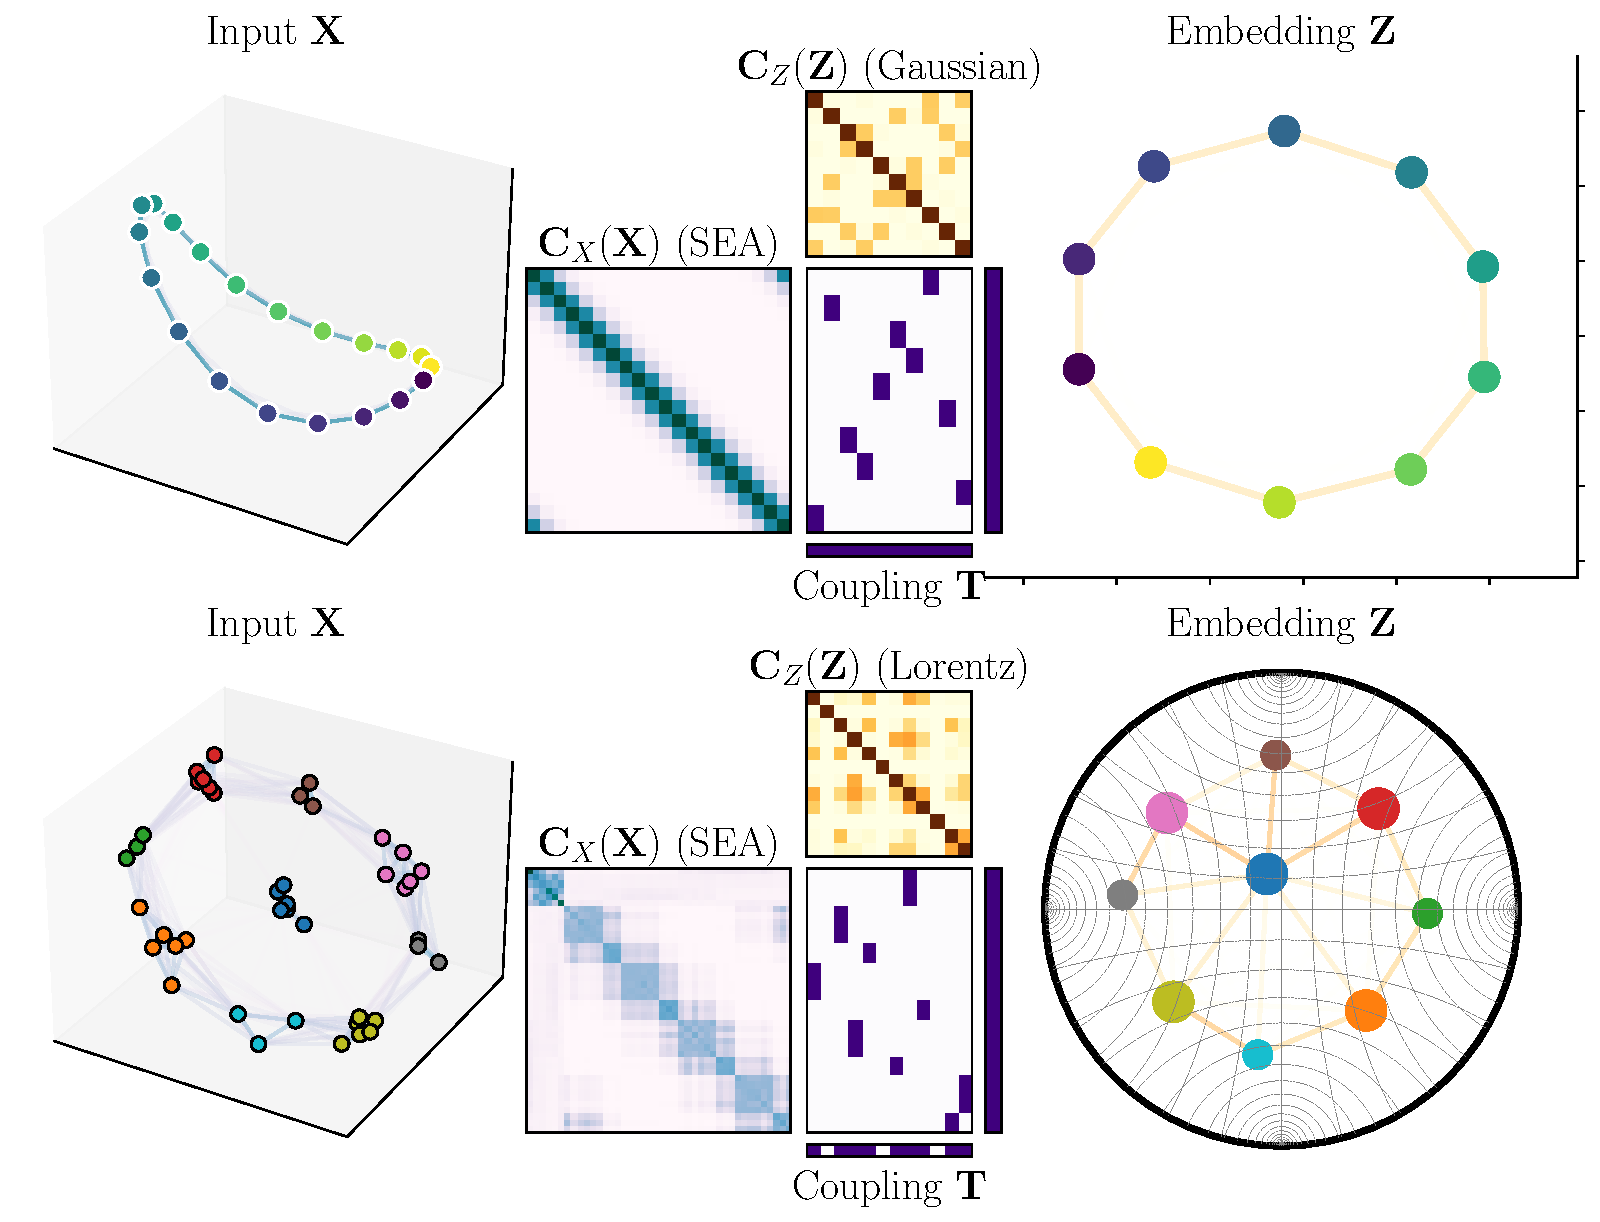
\includegraphics[width=\columnwidth]{figures/DistR/fig_general.pdf}}
	\caption{\textbf{Illustration of our \ref{eq:Dist-DR} method} on two toys examples: points arranged on a circle ({\em top row}) and clusters with varying sizes ({\em bottom}) both in 3 dimensions. {\em Middle column}: input similarity matrix $\mC_X(\mX)$ and final resulting embedding similarity $\mC_Z(\mZ)$. Both are coupled through the coupling matrix $\mT$ (depicted in purple, with its marginals)}
	\label{fig:general_idea}
	\end{center}
	\vskip -0.3in
\end{figure}

This work addresses \Cref{prob:ot_unsupervised} and aims to provide a general formulation of unsupervised representation learning methods as an OT variational problem over a measure. Of particular interest are clustering and dimensionality reduction approaches, both of which are popular ways to summarize datasets. Interestingly, methods from both families share many similitudes, %among which is
including the construction of a similarity graph between input samples. In clustering, many popular approaches design a reduced or coarsened version of the initial similarity graph while preserving some of its spectral properties~\citep{von2007tutorial, schaeffer2007graph}. 
%attributes related to the graph spectrum 
In DR, the goal is to solve the inverse problem of finding low-dimensional embeddings that generate a similarity graph close to the %initial
one computed from input data points \citep{ham2004kernel,hinton2002stochastic}.
%With so many similarities
Our work builds on these converging viewpoints and addresses the following question: \emph{can DR and clustering  be expressed in a common and unified framework ?}

\paragraph{A distributional perspective.} To answer this question, we
propose to look at both problems from a distributional point of view, treating the data as an empirical probability distribution
$\mu=\frac{1}{N}\sum_i\delta_{\vx_i}$. 
% instead of a data matrix. 
This enables us to consider statistical measures of similarity such as Optimal Transport (OT), which is at the core of our work.
On the one hand, OT and clustering are strongly related.
The celebrated K-means approach can be seen as a particular case of minimal Wasserstein estimator where a distribution of $n$ Diracs is optimized \textit{w.r.t} their weights and positions \citep{Canas12}. Other connections between spectral clustering and the OT-based Gromov-Wasserstein (GW) distance have been recently developed in \citep{chowdhury2021generalized,chen2023gromov,vincent2021semi}. On the other hand, the link between DR and OT has not been explored yet. DR methods, when modeling data as distributions,
usually focus on joint distribution between samples within each space separately, see \eg \Cref{chapter:SNEkhorn} of this thesis or \citep{lu2019doubly}.
Consequently, they do not consider couplings to transport samples across spaces of varying dimensions. %To the best of our knowledge, DR methods, when modeling data as distributions,
%focus on joint distribution between samples within each space separately, see \eg \citet{van2023snekhorn} or \citet{lu2019doubly}.
%However, they do not consider couplings to transport samples across spaces of varying dimensions,% thus the link between DR and OT has not been explored yet.
% they do not consider a
% minimal divergence estimator and 

\paragraph{Our contributions.} In this paper, we propose to bridge this gap by
proposing a novel and general distributional framework that encompasses both DR and clustering
as special cases. We notably cast those problems as finding a reduced distribution that minimizes the GW divergence from the original empirical data distribution.
Our method proceeds by first constructing an input similarity matrix
$\mC_X(\mX)$ that is matched with the embedding similarity $\mC_Z(\mZ)$ through
an OT coupling matrix $\mT$. The latter establishes correspondences between
input and embedding samples. We illustrate this principle in
Figure~\ref{fig:general_idea} where one can notice that $\mC_Z(\mZ)$ preserves
the topology of $\mC_X(\mX)$ with a reduced number of nodes. The adaptivity of
our model that can select an effective number of cluster $<n$, is visible in the
bottom plot, where only the exact number of clusters in the original data ($9$ out of the $12$
initially proposed) is automatically recovered. Our method can operate in any embedding space, which is illustrated by
projecting in either a 2D Euclidean plane or a Poincaré ball as embedding
spaces.

We show that this framework is versatile and allows to recover many popular DR
methods such as the kernel PCA and neighbor embedding algorithms, but also clustering 
algorithms such as K-means and spectral clustering. We first prove in Section
\ref{sec:DR_as_OT} that DR can be formulated as a GW projection problem under
some conditions on the loss and similarity functions. We then propose in Section
\ref{sec:DDR} a novel formulation of data summarization as a minimal GW estimator that allows
to select both the dimensionality of the embedding $d$ (DR) but also the number of Diracs
$n$ (Clustering).
% hence providing jointly DR and clustering. 
%Finally, we show in Section \ref{sec:exps} the practical interest and generality of our approach by evaluating its performance on a joint DR/Clustering task and comparing it to existing methods.
Finally, we show in section \ref{sec:exps_distr} the practical interest of our approach, which regularly outperforms its competitors for various joint DR/Clustering tasks.
% \hva{à atténuer un peu:}
% We also illustrate the generality by investigating particularly novel DR methods that optimize the GW divergence in an Eulerian way, with a reduced distribution of fixed support \nc{such as} regular grids (images) or on other supports that can encode prior knowledge.

% Summarizing a dataset in an unsupervised way is of utmost importance in modern machine learning pipelines \citep{donoho2000high}. Reduced data representations offer numerous advantages, including improved pattern and structure recognition as well as faster processing for downstream tasks \citep{pochet2004systematic, mendible2020dimensionality, cantini2021benchmarking}.

% To construct such representations, one can either reduce the sample size by aggregating points together (referred to as \emph{clustering}) or reduce the feature dimensionality \textit{i.e.}\ performing \emph{dimensionality reduction} (DR). 
% Both tasks are actively studied topics and %interestingly
% their inner workings share key mechanisms, %among which is
% like the construction of a similarity graph between input samples.
%  \cvc{(missing high level motivation about why one would want to do so?)}
% However current formulations of DR do not permit adapting the sample size of the resulting embedding. 
% In other words, there does not exist a consistent model allowing to adapt current state-of-the-art DR algorithms to simultaneously perform clustering. As a result, clustering and DR are performed sequentially \cvc{(need to outline limitations of sequential approach)}. 
% In cell biology, for instance, similar cells are grouped into \emph{metacells} \citep{baran2019metacell} that are then embedded onto a low-dimensional space for visualization and other downstream tasks.
% This may result in clusters that are not adapted to the final embedding space and vice versa \citep{liu2022joint} \cvc{(maybe the example should come sooner)}.

% \textbf{Contributions.}
% In this work, we uncover the link between popular DR methods and the Gromov-Wasserstein optimal transport problem \citep{memoli2011gromov}. \cvc{This leads us to frame DR as a novel optimization problem over any discrete distributions, \emph{a.k.a} Distributional Dimensionality Reduction, that provides a first grounded approch for joint DR and clustering.} This novel characterization allows us to frame DR as an optimization problem over discrete distributions offering enhanced flexibility. In particular, it allows one to choose the resolution of the output thus providing a grounded approach for joint dimensionality reduction and clustering. Our contributions can be summarized as follows.
% \begin{itemize}
% 	\item In \Cref{sec:DRasOT}, we provide conditions on the loss and similarity functions under which DR can be equivalently formulated as the GW projection of the empirical data distribution.
% 	\item In \Cref{sec:DDR}
	
% 	\item In \Cref{sec:exps}, we showcase the relevance of our approach for summarizing real datasets composed of images and single-cell data. Compared with existing benchmarks, we show that our model achieves the best trade-off between structure preservation and homogeneity of the obtained clusters.
% \end{itemize} 
% !TeX root = ../paper.tex


\section{Symmetric Entropic Affinities}\label{sec:sym_entropic_affinity}

In this section, we present our first major contribution: symmetric entropic affinities. We begin by providing a new perspective on EAs through the introduction of an equivalent convex problem.

\subsection{Entropic Affinities as Entropic Optimal Transport}\label{sec:entropic_affinity_semi_relaxed}

We introduce the following set of matrices with row-wise stochasticity and entropy constraints:
\begin{align}
  \mathcal{H}_\xi = \{\Pb \in \mathbb{R}_+^{n \times n} \ \text{s.t.} \ \Pb \bm{1} = \bm{1} \: \ \text{and} \  \forall i, \: \operatorname{H}(\Pb_{i:}) \geq \log{\xi} + 1 \}\:.
\end{align}
This space is convex since $\mathbf{p} \in \R_+^n \mapsto \operatorname{H}(\mathbf{p})$ is concave, thus its superlevel set is convex. In contrast to the entropic constraints utilized in standard entropic optimal transport which set a lower-bound on the \emph{global} entropy, as demonstrated in the formulation \eqref{eq:entropy_constrained_OT}, $\mathcal{H}_\xi$ imposes a constraint on the entropy of \emph{each row} of the matrix $\Pb$.
Our first contribution is to prove that EAs can be computed by solving a specific problem involving $\mathcal{H}_\xi$ (see Appendix \ref{sec:proofs} for the proof).
\begin{restatable}{proposition}{entropicaffinityaslinearprogram}
\label{prop:entropic_affinity_as_linear_program}
Let $\Cb \in \R^{n \times n}$ without constant rows. Then $\Pb^{\mathrm{e}}$ solves the entropic affinity problem (\ref{eq:entropic_affinity_pb}) with cost $\Cb$ if and only if $\Pb^{\mathrm{e}}$ is the unique solution of the convex problem
\begin{equation}\label{eq:entropic_affinity_semi_relaxed}
    \min_{\Pb \in \mathcal{H}_{\xi}} \: \langle \Pb, \Cb \rangle .
    \tag{EA as OT}
\end{equation}
\end{restatable}
Interestingly, this result shows that EAs boil down to minimizing a transport objective with cost $\Cb$ and row-wise entropy constraints $\mathcal{H}_{\xi}$ where
$\xi$ is the desired perplexity. As such, \eqref{eq:entropic_affinity_semi_relaxed} can be seen as a specific \emph{semi-relaxed} OT problem \citep{rabin2014adaptive,flamary2016optimal} (\ie without the second constraint on the marginal $\Pb^\top \bm{1}= \bm{1}$) but with entropic constraints on the rows of $\Pb$. We also show that the optimal solution $\Pb^\star$ of \eqref{eq:entropic_affinity_semi_relaxed} has \emph{saturated entropy} \ie $\forall i, \: \operatorname{H}(\Pb^\star_{i:}) = \log{\xi} + 1$. In other words, relaxing the equality constraint in \eqref{eq:entropic_affinity_pb} as a inequality constraint in $\Pb \in \mathcal{H}_{\xi}$ does not affect the solution while it allows reformulating entropic affinity as a convex optimization problem. To the best of our knowledge, this connection between OT and entropic affinities is novel and is an essential key to the method proposed in the
next section.
% To gain intuition on the entropy saturation at the optimum, one can simply notice that, since $\Cb \in
% \mathcal{D}$, transferring some mass from anywhere off-diagonal to the diagonal
% decreases both the objective and the entropy.

\begin{remark}
  The kernel bandwidth parameter $\bm{\varepsilon}$ from the original formulation of entropic affinities (\ref{eq:entropic_affinity_pb}) is the Lagrange dual variable associated with the entropy constraint in (\ref{eq:entropic_affinity_semi_relaxed}). Hence computing $\bm{\varepsilon}^\star$ in (\ref{eq:entropic_affinity_pb}) exactly corresponds to solving the dual problem of (\ref{eq:entropic_affinity_semi_relaxed}).
\end{remark}

\begin{remark}\label{Pe_proj}
  Let $\K_{\sigma} = \exp(-\Cb / \sigma)$. As shown in \cref{sec:proj_KL}, if $\bm{\varepsilon}^\star$ solves (\ref{eq:entropic_affinity_pb}) and $\sigma \leq \min(\bm{\varepsilon}^\star)$, then $\Pb^{\mathrm{e}} = \operatorname{Proj}^{\operatorname{\KL}}_{\mathcal{H}_{\xi}}(\K_{\sigma})  =  \argmin_{\Pb \in \mathcal{H}_{\xi}} \KL(\Pb | \K_\sigma)$.
  Therefore $\Pb^{\mathrm{e}}$ can be seen as a $\KL$ Bregman projection \citep{benamou2015iterative} of a Gaussian kernel onto $\mathcal{H}_{\xi}$. Hence the input matrix in \eqref{symmetrization_tsne}  is $\overline{\Pb^{\mathrm{e}}}= \operatorname{Proj}^{\ell_2}_{\mathcal{S}}(\operatorname{Proj}^{\operatorname{\KL}}_{\mathcal{H}_{\xi}}(\K_\sigma))$ which corresponds to a surprising mixture of $\KL$ and orthogonal projections.
\end{remark}

\subsection{Symmetric Entropic Affinity Formulation}\label{subsec:sea}

\begin{figure*}[t]
  \begin{center}
  \centerline{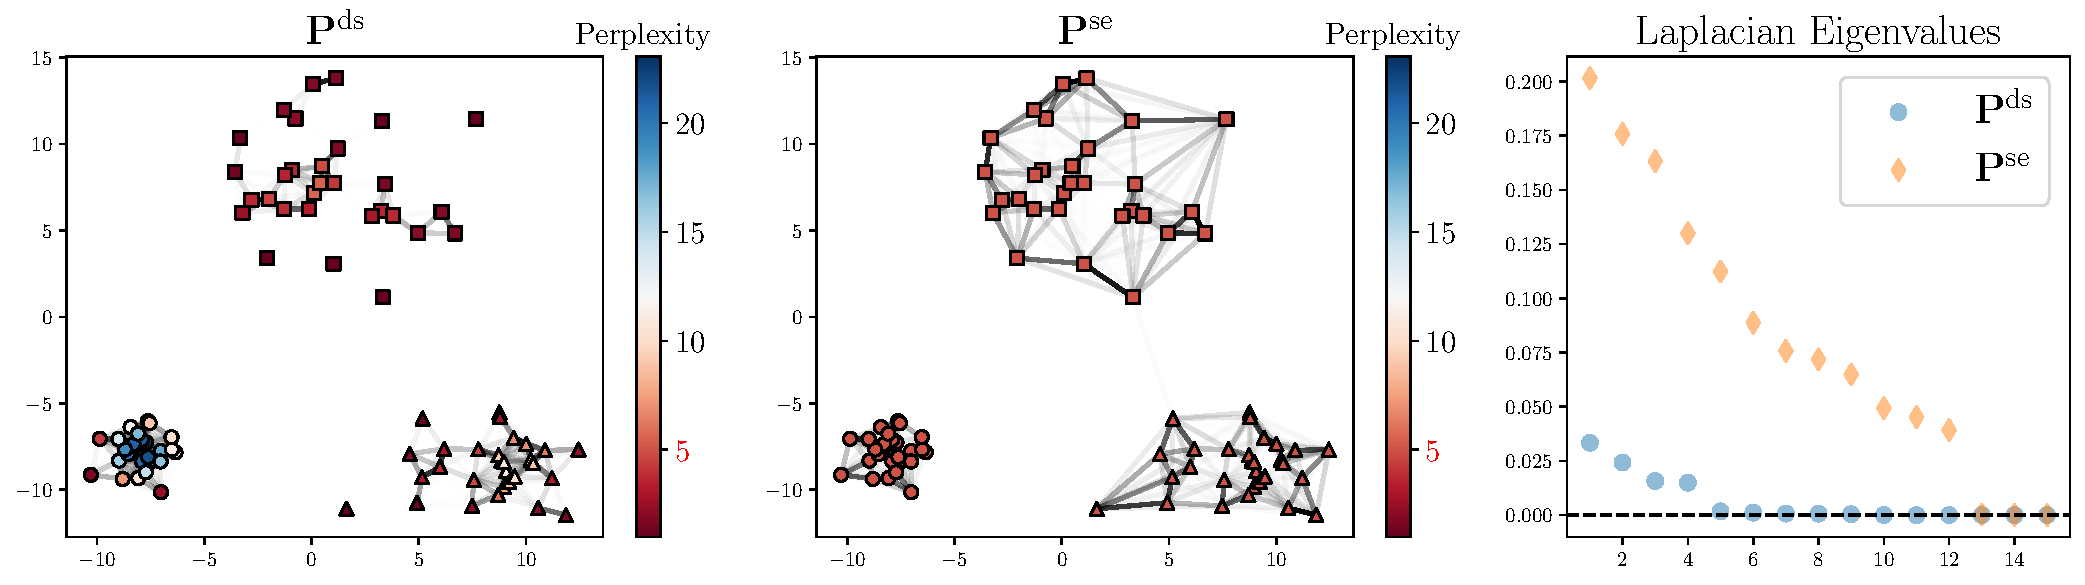
\includegraphics[width=\columnwidth]{figures/SNEkhorn/Ps_vs_Pse.pdf}}
  \caption{Samples from a mixture of three Gaussians with varying standard deviations. The edges' strength is proportional to the weights in the affinities $\Pb^{\mathrm{ds}}$ \eqref{eq:plan_sym_sinkhorn} and $\Pb^{\mathrm{se}}$ \eqref{eq:sym_entropic_affinity} computed with $\xi=5$ (for $\Pb^{\mathrm{ds}}$, $\xi$ is the average perplexity such that $\sum_i \operatorname{H}(\Pb^{\mathrm{ds}}_{i:})=\sum_i \operatorname{H}(\Pb^{\mathrm{se}}_{i:})$). Points' color represents the perplexity $e^{\operatorname{H}(\Pb_{i:})-1}$. Right plot: smallest eigenvalues of the Laplacian for the two affinities.}
  \label{fig:Ps_vs_Pse}
  \end{center}
\end{figure*}

Based on the previous formulation we now propose symmetric entropic affinities: a symmetric version of EAs that enables keeping the entropy associated with each row (or equivalently column) to the desired value of $\log \xi + 1$ while producing a symmetric doubly stochastic affinity matrix. Our strategy is to enforce symmetry through an additional constraint in (\ref{eq:entropic_affinity_semi_relaxed}), in a similar fashion as \eqref{eq:entropy_constrained_OT}. More precisely we consider the convex optimization problem
\begin{align}
\label{eq:sym_entropic_affinity}
\tag{SEA}
  \min_{\Pb \in \mathcal{H}_{\xi} \cap \mathcal{S}} \: \langle \Pb, \Cb \rangle \:. 
\end{align}
where we recall that $\mathcal{S}$ is the set of $n \times n$ symmetric matrices. Note that for any $\xi \leq n-1$, $\frac{1}{n} \bm{1}\bm{1}^\top \in \mathcal{H}_{\xi} \cap \mathcal{S}$ hence the set $\mathcal{H}_{\xi} \cap \mathcal{S}$ is a non-empty and convex set. We first detail some important properties of problem \eqref{eq:sym_entropic_affinity} (the proofs of the following results can be found in Appendix \ref{proof:main_props}).
\begin{restatable}[Saturation of the entropies]{proposition}{saturation}
\label{prop:saturation_entropies}
Let $\Cb \in \mathcal{S}$ with zero diagonal, then \eqref{eq:sym_entropic_affinity} with cost $\Cb$ has a \emph{unique solution} that we denote by $\Pb^{\mathrm{se}}$. If moreover $\Cb \in \mathcal{D}$, then for at least $n-1$ indices $i \in \integ{n}$ the solution satisfies $\operatorname{H}(\Pb^{\mathrm{se}}_{i:}) = \log \xi + 1$.
\end{restatable}
In other words, the unique solution $\Pb^{\mathrm{se}}$ has at least $n-1$ saturated entropies \ie the corresponding $n-1$ points have exactly a perplexity of $\xi$. In practice, with the algorithmic solution detailed below, we have observed that all $n$ entropies are saturated. Therefore, we believe that this proposition can be extended with a few more assumptions on $\Cb$. Accordingly,
problem \eqref{eq:sym_entropic_affinity} allows accurate control over the point-wise entropies while providing a symmetric doubly stochastic matrix, unlike $\overline{\Pb^{\mathrm{e}}}$ defined in
\eqref{symmetrization_tsne}, as summarized in \cref{recap_properties_sym}. In the sequel, we denote by $\operatorname{H}_{\mathrm{r}}(\Pb) = \left( \operatorname{H}(\Pb_{i:}) \right)_{i}$ the vector of row-wise entropies of $\Pb$. We rely on the following result to compute $\Pb^{\mathrm{se}}$.
\begin{restatable}[Solving for \ref{eq:sym_entropic_affinity}]{proposition}{solvingsea}
\label{prop:sol_gamma_non_null}
Let $\Cb \in \mathcal{D}, \mathcal{L}(\Pb, \bm{\gamma}, \bm{\lambda})= \langle \Pb, \Cb \rangle + \langle \gammab, (\log{\xi} + 1) \bm{1} - \operatorname{H}_{\mathrm{r}}(\Pb) \rangle + \langle \lambdab, \bm{1} - \Pb \bm{1} \rangle$ and $q(\bm{\gamma}, \bm{\lambda}) = \min_{\Pb \in \R_{+}^{n \times n} \cap \mathcal{S}} \mathcal{L}(\Pb, \bm{\gamma}, \bm{\lambda})$. Strong duality holds for \eqref{eq:sym_entropic_affinity}. Moreover, let
$\bm{\gamma}^\star, \lambdab^\star \in \operatorname{argmax}_{\bm{\gamma} \geq 0, \lambdab} q(\bm{\gamma}, \bm{\lambda})$ be the optimal dual variables respectively associated with the entropy and marginal constraints. Then, for at least $n-1$ indices $i \in \integ{n}, \gamma^{\star}_i > 0$.
When $\forall i \in \integ{n}$, $\gamma^\star_i > 0$ then $\operatorname{H}_{\mathrm{r}}(\Pb^{\mathrm{se}}) = (\log \xi + 1)\bm{1}$ and $\Pb^{\mathrm{se}}$ has the form
\begin{align}
    \Pb^{\mathrm{se}} &= \exp{\left(\left(\lambdab^\star \oplus \lambdab^\star - 2 \Cb \right) \oslash \left(\bm{\gamma}^\star \oplus \bm{\gamma}^\star \right) \right)} \:.
   % \label{eq:optimal_P_se}
\end{align}
\end{restatable}
% To set the dual variables to their optimal value, a direct approach consists in solving the following dual problem which is concave, denoting $\Pb^{\star}(\gammab, \lambdab) = \exp{\left(\left(\lambdab \oplus \lambdab - 2 \Cb \right) \oslash \left(\bm{\gamma} \oplus \bm{\gamma} \right) \right)}$.
% \begin{align}\label{eq:dual_problem}\tag{Dual-SEA}
%   \max_{\gammab, \lambdab} \: \min_{\Pb \in \mathcal{S}} \quad \langle \Pb, \Cb \rangle + \langle \gammab, (\log{\xi} + 1) \bm{1} - \operatorname{H}_{\mathrm{r}}(\Pb) \rangle + \langle \lambdab, \bm{1} - \Pb \bm{1} \rangle \:.
% \end{align}
% \begin{align}\label{eq:dual_problem}\tag{Dual-SEA}
%   \max_{\gammab \bm{>} \bm{0}, \lambdab}  \quad \langle \Pb^\star(\gammab, \lambdab), \Cb \rangle + \langle \gammab, (\log{\xi} + 1) \bm{1} - \bm{h}^\star(\gammab, \lambdab) \rangle + \langle \lambdab, \bm{1} - \Pb^\star(\gammab, \lambdab) \bm{1} \rangle
% \end{align}
% \begin{proposition}[Unicity and entropy of the solution]\label{prop:sol_sym_perp}
%   \eqref{eq:sym_entropic_affinity} has a unique solution denoted $\Pb^{\mathrm{se}}$. Moreover, for at least $n-1$ indices $i \in \integ{n}$, it holds $\operatorname{H}(\Pb^{\mathrm{se}}_{i:}) = \log \xi + 1$.
% \end{proposition}
% This has minor impacts on the overall control of the entropies especially when $n$ is large. 
% \hug{faux et on a abandonné:
% Moreover, in appendix \ref{sec:all_entropies_saturated}, we provide a sufficient condition on $\Cb$ for $\operatorname{H}(\Pb^{\mathrm{se}}_{i:}) = \log \xi + 1$ to hold for any $i \in \integ{n}$. We found this condition to be mild in practice.}
% Though we did not manage to prove it rigorously, 
By defining the symmetric matrix $\Pb(\bm{\gamma}, \bm{\lambda}) = 
\exp{\left(\left(\lambdab \oplus \lambdab - 2 \Cb \right) \oslash \left(\bm{\gamma} \oplus \bm{\gamma} \right) \right)}$, we prove that, when $\bm{\gamma}>0, \min_{\Pb \in \mathcal{S}} \mathcal{L}(\Pb, \bm{\gamma}, \bm{\lambda})$ has a unique solution given by $\Pb(\bm{\gamma}, \bm{\lambda})$ which implies $q(\gammab, \lambdab) = \mathcal{L}(\Pb(\bm{\gamma}, \bm{\lambda}), \gammab, \lambdab)$. Thus the proposition shows that when $\bm{\gamma}^\star > 0, \ \Pb^{\mathrm{se}} = \Pb(\bm{\gamma}^\star, \bm{\lambda}^\star)$ where $\bm{\gamma}^\star, \bm{\lambda}^\star$ solve the \emph{concave} dual problem 
\begin{equation}
\label{eq:dual_problem}
\tag{Dual-SEA}
\max_{\bm{\gamma} > 0, \lambdab} \mathcal{L}(\Pb(\bm{\gamma}, \bm{\lambda}), \bm{\gamma}, \bm{\lambda}). 
% \text{ where } \Pb(\bm{\gamma}, \bm{\lambda}) := 
% \exp{\left(\left(\lambdab \oplus \lambdab - 2 \Cb \right) \oslash \left(\bm{\gamma} \oplus \bm{\gamma} \right) \right)}
\end{equation}
% As stated in the above result, one can easily see that our proposed
% symmetrization always provides guarantees over the saturation of $n-1$ entropies
% at the optimum. Indeed, let us imagine that there exists two rows $(\ell,
% \ell')$ for which the entropies are strictly greater than $\log \xi + 1$. 
% \begin{wraptable}[9]{R}{7cm}
%   \caption{Properties of $\Pb^{\mathrm{e}}$, $\overline{\Pb^{\mathrm{e}}}$, $\Pb^{\mathrm{ds}}$ and $\Pb^{\mathrm{se}}$}
%   % \begin{small}
%   %  \begin{minipage}{7cm}
%   \begin{sc} \setlength\tabcolsep{1mm}
%   \begin{tabular}{lcccc}
%   \toprule[1.5pt]
% Affinity matrix& $\Pb^{\mathrm{e}}$& $\overline{\Pb^{\mathrm{e}}}$
%   & $\Pb^{\mathrm{ds}}$& $\Pb^{\mathrm{se}}$ \\
%   Reference & \citep{hinton2002stochastic} & \citep{van2008visualizing} & \citep{lu2019doubly} & \eqref{eq:sym_entropic_affinity} \\
%   \midrule
%   $\Pb=\Pb^\top$ & $\red{\boldsymbol\times}$ & $\green{\Cbheckmark}$ & $\green{\Cbheckmark}$ & $\green{\Cbheckmark}$ \\
%   $\Pb \bm{1} = \Pb^\top \bm{1} = \bm{1}$ & $\red{\boldsymbol\times}$ & $\red{\boldsymbol\times}$ & $\green{\Cbheckmark}$ & $\green{\Cbheckmark}$ \\
%   $\operatorname{H}_{\mathrm{r}}(\Pb) = (\log \xi + 1)\bm{1}$ & $\green{\Cbheckmark}$ & $\red{\boldsymbol\times}$ & $\red{\boldsymbol\times}$ & $\green{\Cbheckmark}$ \\
%   \bottomrule[1.5pt]
%   \label{recap_properties_sym}
%   \end{tabular}
%   \end{sc}
% %\end{minipage}
%   % \end{small}
%   %\vspace{10mm}
% \end{wraptable}

% To prove this result the main idea is to use that $\Cb$ has zero diagonal Indeed, let us imagine that there exists two rows $(\ell,
% \ell')$ for which the entropies are strictly greater than $\log \xi + 1$. 
% Then, transferring some mass from $\Pb^{\mathrm{se}}_{\ell \ell'}$ and
% $\Pb^{\mathrm{se}}_{\ell' \ell}$ (evenly to keep the symmetry) to the diagonal
% would decrease both the cost and the entropies in rows $\ell$ and $\ell'$. Thus
% one can apply this transformation to decrease the objective until one of the two
% rows reaches the lower bound value $\log \xi + 1$. This reasoning intuitively
% shows that there can not be more than one unsaturated entropy at the optimum. 
% It also proves that $\bm{\gamma}^\star_i > 0$ for at least $n-1$ indices. 
% For all the real-world cases that we considered (see Section \ref{sec:DR_experiments}), we found that the optimum of \eqref{eq:dual_problem} had indeed $n$ saturated entropies.
Consequently, to find $\Pb^{\mathrm{se}}$ we solve the problem \eqref{eq:dual_problem}. Although the form of $\Pb^{\mathrm{se}}$ presented in Proposition \ref{prop:sol_gamma_non_null} is only valid when $\bm{\gamma}^\star$ is positive and we have only proved it for $n-1$ indices, we emphasize that if \eqref{eq:dual_problem} has a finite solution, then it is equal to $\Pb^{\mathrm{se}}$. Indeed in this case the solution satisfies the KKT system associated with \eqref{eq:sym_entropic_affinity}.
  
\begin{table}
\begin{center}
\caption{Properties of $\Pb^{\mathrm{e}}$, $\overline{\Pb^{\mathrm{e}}}$, $\Pb^{\mathrm{ds}}$ and $\Pb^{\mathrm{se}}$.}
  \begin{tabular}{lcccc}
  \toprule[1.5pt]
  Affinity matrix& $\Pb^{\mathrm{e}}$& $\overline{\Pb^{\mathrm{e}}}$
  & $\Pb^{\mathrm{ds}}$& $\Pb^{\mathrm{se}}$ \\
  % Reference & \citep{hinton2002stochastic} & \citep{van2008visualizing} & \citep{lu2019doubly} & \eqref{eq:sym_entropic_affinity} \\
  \midrule
  $\Pb=\Pb^\top$ & $\red{\boldsymbol\times}$ & $\green{\checkmark}$ & $\green{\checkmark}$ & $\green{\checkmark}$ \\
  $\Pb \bm{1} = \Pb^\top \bm{1} = \bm{1}$ & $\red{\boldsymbol\times}$ & $\red{\boldsymbol\times}$ & $\green{\checkmark}$ & $\green{\checkmark}$ \\
  $\operatorname{H}_{\mathrm{r}}(\Pb) = (\log \xi + 1)\bm{1}$ & $\green{\checkmark}$ & $\red{\boldsymbol\times}$ & $\red{\boldsymbol\times}$ & $\green{\checkmark}$ \\
  \bottomrule[1.5pt]
  \end{tabular}
  \end{center}
\end{table}


\paragraph{Numerical optimization.} The dual problem \eqref{eq:dual_problem} is concave and can be solved with guarantees through a dual ascent approach with closed-form gradients (using \eg \texttt{SGD}, \texttt{BFGS} \citep{liu1989limited} or \texttt{ADAM} \citep{kingma2014adam}).
% (as depicted in algorithm \ref{algo:dual_ascent})
% \begin{align*}
%     \nabla_{\bm{\gamma}} \mathcal{G}(\bm{\gamma}, \bm{\lambda}) &= (\log \xi + 1 )\bm{1} - \operatorname{H}_{\mathrm{r}}(\Pb^\star(\bm{\gamma}, \bm{\lambda})) \\
%     \nabla_{\bm{\lambda}} \mathcal{G}(\bm{\gamma}, \bm{\lambda}) &= \bm{1} - \Pb^\star(\bm{\gamma}, \bm{\lambda}) \bm{1} \:.
% \end{align*}
%A pseudo-code for this method is provided in \cref{algo:dual_ascent}. 
At each gradient step, one can compute the current estimate $\Pb(\bm{\gamma}, \bm{\lambda})$ while the gradients of the loss \textit{w.r.t.} $\gammab$ and $\lambdab$ are given respectively by the constraints $(\log{\xi}+1)
\bm{1} - \operatorname{H}_{\mathrm{r}}(\Pb(\bm{\gamma}, \bm{\lambda}))$ and $ \bm{1} - \Pb(\bm{\gamma}, \bm{\lambda}) \bm{1}$ (see \eg \cite[Proposition 6.1.1]{bertsekas1997nonlinear}).
Concerning time
complexity, each step can be performed with $\mathcal{O}(n^2)$ algebraic
operations. From a practical perspective, we found that using a change of variable $\gammab \leftarrow \gammab^2$ and optimize $\gammab \in \R^n$ leads to enhanced numerical stability.
%  In all the practical cases that we considered, we
% found that \cref{algo:dual_ascent} converged and effectively solved
% \eqref{eq:sym_entropic_affinity} thus proving that $\bm{\gamma}^\star \bm{>}
% \bm{0}$ for these cases. 
%Characterizing theoretically the conditions to have
%$\bm{\gamma}^\star \bm{>} \bm{0}$ remains an open problem.
% Note that upon convergence, the
% algorithm provides a solution satisfying the KKT system of
% \eqref{eq:sym_entropic_affinity} thus solving \eqref{eq:sym_entropic_affinity}
% by convexity of the problem.

\begin{remark}
  In the same spirit as \cref{Pe_proj}, one can express $\Pb^{\mathrm{se}}$ as a $\KL$ projection of $\K_{\sigma} = \exp(-\Cb/\sigma)$.
  Indeed, we show in \cref{sec:proj_KL} that if $0 < \sigma \leq \min_i \gamma^\star_i$, then $\Pb^{\mathrm{se}} = \operatorname{Proj}^{\operatorname{\KL}}_{\mathcal{H}_{\xi} \cap
  \mathcal{S}}(\K_{\sigma})$. This characterization opens the door for alternating Bregman projection methods (described in \cref{sec:dykstra}) which were not found to be more efficient than dual ascent.
\end{remark}

\textbf{Comparison between $\Pb^{\mathrm{ds}}$ and $\Pb^{\mathrm{se}}$.} In \cref{fig:Ps_vs_Pse} we illustrate the ability of our proposed affinity $\Pb^{\mathrm{se}}$ to adapt to varying noise levels. In the OT problem that we consider, each sample is given a mass of one that is distributed over its neighbors (including itself since self-loops are allowed). For each sample, we refer to the entropy of the distribution over its neighbors as the \emph{spreading} of its mass. One can notice that for $\Pb^{\mathrm{ds}}$ \eqref{eq:plan_sym_sinkhorn} 
(OT problem with global entropy constraint \eqref{eq:entropy_constrained_OT})
, the samples do not spread their mass evenly depending on the density around them. On the contrary, the per-row entropy constraints of $\Pb^{\mathrm{se}}$ force equal spreading among samples.
% thereby adapting to the variance of each cluster. 
This can have benefits, particularly for clustering, as illustrated in the rightmost plot, which shows the eigenvalues of the associated Laplacian matrices (recall that the number of connected components equals the dimension of the null space of its Laplacian \citep{chung1997spectral}). As can be seen, $\Pb^{\mathrm{ds}}$ results in many unwanted clusters, unlike $\Pb^{\mathrm{se}}$, which is robust to varying noise levels (its Laplacian matrix has only $3$ vanishing eigenvalues). 

% !TeX root = ../paper.tex

\section{Optimal Transport for Dimension Reduction with SNEkhorn}\label{sec:DR_with_OT}

In this section, we build upon symmetric entropic affinities to introduce SNEkhorn, a new DR algorithm that fully benefits from the advantages of doubly stochastic affinities.

\paragraph{SNEkhorn's objective.} Our proposed method relies on doubly stochastic affinity matrices to capture the dependencies among the samples in both input \emph{and} latent spaces. The $\KL$ divergence, which is the central criterion in most popular DR methods \cite{van2022probabilistic}, is used to measure the discrepancy between the two affinities. As detailed in sections \ref{sec:background} and \ref{sec:sym_entropic_affinity}, $\Pb^{\mathrm{se}}$ corrects for heterogeneity in the
data density by imposing point-wise entropy constraints. As we do not need such correction for embedding coordinates $\Z$ since they must be optimized, we opt for the standard affinity \eqref{eq:plan_sym_sinkhorn} built as an OT transport plan with global entropy constraint \eqref{eq:entropy_constrained_OT}. This OT plan can be efficiently computed using Sinkhorn's algorithm. More precisely, 
% considering $\C_\X$ and $\C_{\Zb}$  the pairwise cost matrices of $\X$ and $\Z$ respectively, 
we propose the optimization problem
\begin{align}\label{coupling_pb}
    \min_{\Zb \in \mathbb{R}^{n \times q}} \:  \mathrm{KL}\big(\Pb^{\mathrm{se}} | \mathbf{Q}^{\mathrm{ds}}_{\Zb} \big)\,,
\tag{SNEkhorn}
\end{align}
where $\mathbf{Q}^{\mathrm{ds}}_{\Zb} = \exp \left(\mathbf{f}_{\Zb} \oplus \mathbf{f}_{\Zb} - \C_{\Zb} \right)$ stands for the $\eqref{eq:plan_sym_sinkhorn}$ affinity computed with cost $\C_{\Zb}$ and $\mathbf{f}_{\Zb}$ is the optimal dual variable found by Sinkhorn's algorithm.
% In the above, $\Pb^{\mathrm{se}}_{\xi}(\C_\X)$ stands for the \eqref{eq:sym_entropic_affinity} matrix associated to the cost $\C_\X$ with perplexity $\xi$. 
We set the bandwidth to $\nu = 1$ in $\Qb^{\mathrm{ds}}_{\Zb}$ similarly to \cite{van2008visualizing} as the bandwidth in the low dimensional space only affects the scales of the embeddings and not their shape.
Keeping only the terms that depend on $\Z$ and relying on the double stochasticity of $\Pb^{\mathrm{se}}$, the objective in (\ref{coupling_pb}) can be expressed as $\langle \Pb^{\mathrm{se}}, \C_{\Zb} \rangle - 2 \langle \mathbf{f}_{\Zb}, \bm{1} \rangle$. %In this decomposition, the left term settles attractive forces and the right term repulsive ones. pas tres clair j'enelve

\paragraph{Heavy-tailed kernel in latent space.}
Since it is well known that heavy-tailed kernels can be beneficial in DR
\cite{kobak2020heavy}, we propose an extension called t-SNEkhorn that
simply amounts to computing a doubly stochastic student-t kernel 
% $\Tilde{\K} = (\bm{1}\bm{1}^\top + \C)^{\odot -1}$ 
in the low-dimensional space. With our construction, it corresponds to choosing the cost $[\Cb_{\Zb}]_{ij} = \left(\log(1 + \|\Zb_{i:}-\Zb_{j:}\|_2^2)\right)_{ij}$
instead of $(\|\Zb_{i:}-\Zb_{j:}\|_2^2)_{ij}$.

\paragraph{Inference.}
This new DR objective involves computing a doubly stochastic normalization for each update of $\Zb$. Interestingly, to compute the optimal dual variable $\mathbf{f}_{\Zb}$ in $\Qb^{\mathrm{ds}}_{\Zb}$, we leverage a well-conditioned Sinkhorn fixed point iteration \citep{knight2014symmetry, feydy2019interpolating}, which converges extremely fast in the symmetric setting:
\begin{equation}\label{eq:sinkhorn_iterations_log_sym_accelerated}
    \forall i, \: 
    [\mathbf{f}_{\Zb}]_i \leftarrow \frac{1}{2} \left( [\mathbf{f}_{\Zb}]_i - \log \sum_{k} \exp \big([\mathbf{f}_{\Zb}]_k - [\Cb_{\Zb}]_{ki} \big) \right) \:.
\tag{Sinkhorn}
\end{equation}
On the right side of \cref{fig:snekhorn_not_DS}, we plot $\| \Qb^{\mathrm{ds}}_{\Zb} \bm{1} - \bm{1} \|_{\infty}$ as a function of \eqref{eq:sinkhorn_iterations_log_sym_accelerated} iterations for a toy example presented in \cref{sec:DR_experiments}. In most practical cases, we found that about 10 iterations were enough to reach a sufficiently small error. 
$\Zb$ is updated through gradient descent with gradients obtained by performing backpropagation through the Sinkhorn iterations. These
iterations can be further accelerated with a \emph{warm start} strategy by plugging the $\mathbf{f}_{\Zb}$ of the last Sinkhorn to initialize the current one.
% Fortunately, one doesn't need to differentiate through all the unrolled Sinkhorn iterations (\ref{eq:sinkhorn_iterations_log_sym_accelerated}) to compute $\nabla_{\Zb}\f$.
% One can derive the gradient of the objective \textit{w.r.t.}\ $\Z$ as
% \begin{align*}
%     \nabla_{\Zb} \mathcal{J}(\X, \Z) = 2 \left(\Lb \Z - \nabla_{\Zb}\f^{\top} \bm{1} \right) \:.
% \end{align*} 

\begin{minipage}{0.59\linewidth}
        \textbf{Related work.}
        Using doubly stochastic affinities for SNE has been proposed in \cite{lu2019doubly}, with two key differences from our work. First, they
        do not consider EAs and resort to $\Pb^{\mathrm{ds}}$ \eqref{eq:plan_sym_sinkhorn}. This affinity, unlike $\Pb^{\mathrm{se}}$, is not adaptive to the data heterogeneous density (as illusrated in \cref{fig:Ps_vs_Pse}). 
        Second, they use the affinity $\widetilde{\Qb}_{\Zb}$ in the low-dimensional space and demonstrate both empirically and theoretically that matching the latter with a doubly stochastic matrix (\eg $\Pb^{\mathrm{ds}}$ or $\Pb^{\mathrm{se}}$) imposes spherical constraints on the embedding $\Zb$.
        % As a consequence, latent coordinates tend to concentrate on spheres \titouan{pas clair: DS + pas DS = sphere, DS + DS = pas sphere ?}. As a consequence, they focus on building embeddings on spheres in a $3D$ space.
        This is detrimental for projections onto a $2D$ flat space (typical use case of DR) where embeddings tend to form circles. This can be verified on the left side of \cref{fig:snekhorn_not_DS}. In contrast, in SNEkhorn, the latent affinity \emph{is also doubly stochastic} so that latent coordinates $\Zb$ are not subject to spherical constraints anymore.
        The corresponding SNEkhorn embedding is shown in \cref{fig:simulated_data_multinomial} (bottom right).
        % their proposed method called \texttt{DOSNES} does
\end{minipage}
\hspace{0.005\linewidth}
\begin{minipage}{0.4\linewidth} 
\vspace{-0.2cm}
    \centerline{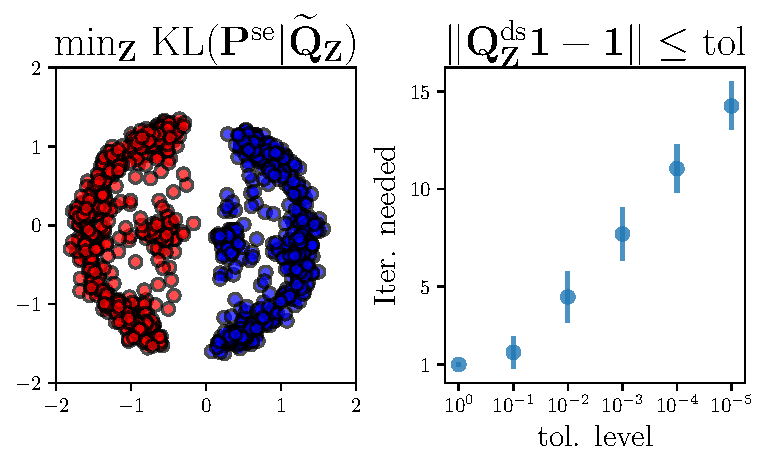
\includegraphics[width=\linewidth]{Figures/snekhorn_not_DS.pdf}}
    \captionof{figure}{Left: SNEkhorn embedding on the simulated data of \cref{sec:DR_experiments} using $\widetilde{\Qb}_{\Zb}$ instead of $\Qb^{\mathrm{ds}}_{\Zb}$ with $\xi=30$. Right: number of iterations needed to achieve $\| \Qb^{\mathrm{ds}}_{\Zb} \bm{1} - \bm{1} \|_{\infty} \leq \text{tol}$ with \eqref{eq:sinkhorn_iterations_log_sym_accelerated}.}
    \label{fig:snekhorn_not_DS}
\end{minipage}

% !TeX root = ../paper.tex
\section{Numerical experiments}\label{sec:DR_experiments}


\begin{figure}
    \centering
    \includegraphics[width=\linewidth]{figures/SNEkhorn/heteroscedastic_noise.pdf}    \caption{From left to right: entries of $\overline{\Pb^{\mathrm{e}}}$ \eqref{symmetrization_tsne} and associated embeddings generated using $\overline{\Pb^{\mathrm{e}}}$. Then $\Pb^{\mathrm{se}}$ \eqref{eq:sym_entropic_affinity} matrix and associated SNEkhorn embeddings. Perplexity $\xi = 30$.}
    \label{fig:simulated_data_multinomial}
\end{figure}

This section aims at illustrating the performances of the proposed affinity
matrix $\Pb^{\mathrm{se}}$ \eqref{eq:sym_entropic_affinity} and DR method SNEkhorn at faithfully representing dependencies and
clusters in low dimensions. First, we showcase the relevance of our approach on a simple synthetic dataset with heteroscedastic noise. 
% (Section
% \ref{sec:simulated_data}). 
Then, we evaluate the spectral clustering
performances of symmetric entropic affinities before benchmarking
t-SNEkhorn with t-SNE and UMAP \cite{mcinnes2018umap} on real-world images and genomics datasets.
% (Section \ref{sec:exp_real_data}).

% \subsection{Simulated data}\label{sec:simulated_data}
% \begin{minipage}{0.48\linewidth} 
% \textbf{Simulated data.}
% We take inspiration from \cite{landa2021doubly} and consider the task of discriminating between samples from two multinomial distributions. We first sample uniformly two vectors $\p_1$ and $\p_2$ in the $10^4$-dimensional probability simplex. We then generate $n=10^3$ samples as $\x_i =\tilde{\x}_i / (\sum_j \tilde{x}_{ij})$ such that:
% \begin{align*}
%     \tilde{\x}_i \sim 
%     \left\{
%     \begin{array}{ll}
%         \mathcal{M}(10^3, \p_1), & 1\leq i \leq 500 \\
%         \mathcal{M}(10^3, \p_2), & 501\leq i \leq 750 \\
%         \mathcal{M}(10^4, \p_2), & 751\leq i \leq 1000 \:.
%     \end{array}
%     \right.
% \end{align*}
% where $\mathcal{M}$ stands for the multinomial distribution. 
% The goal of the task is to test the robustness to heteroscedastic noise. Indeed, points generated using $\p_2$ exhibit different levels of noise due to various numbers of multinomial trials ($10^3$ and $10^4$) to form an estimation of $\p_2$. This typically occurs in real-world scenarios when the same entity is measured using different experimental setups thus creating heterogeneous technical noise levels (\eg in single-cell sequencing \cite{kobak2019art}). This phenomenon is known as \emph{batch effect} \cite{tran2020benchmark}.
% \end{minipage}
% \hspace{0.005\linewidth}
% \begin{minipage}{0.5\linewidth}
% \vspace{-1mm}
% \centering
% \includegraphics[width=\linewidth]{figures/heteroscedastic_noise.pdf}
%  \captionof{figure}{Top: entries of $\overline{\Pb^{\mathrm{e}}}$ \eqref{symmetrization_tsne} and $\Pb^{\mathrm{se}}$ \eqref{eq:sym_entropic_affinity} matrices. Bottom: embeddings generated by symmetric-SNE and SNEkhorn using the above affinities. Perplexity $\xi = 30$.}
% \label{fig:simulated_data_multinomial}
% \end{minipage}

\textbf{Simulated data.}
We take inspiration from \cite{landa2021doubly} and consider the task of discriminating between samples from two multinomial distributions. We first sample uniformly two vectors $\pb_1$ and $\pb_2$ in the $10^4$-dimensional probability simplex. We then generate $n=10^3$ samples as $\xb_i =\tilde{\xb}_i / (\sum_j \tilde{x}_{ij})$ such that:
\begin{align*}
    \tilde{\xb}_i \sim 
    \left\{
    \begin{array}{ll}
        \mathcal{M}(10^3, \pb_1), & 1\leq i \leq 500 \\
        \mathcal{M}(10^3, \pb_2), & 501\leq i \leq 750 \\
        \mathcal{M}(10^4, \pb_2), & 751\leq i \leq 1000 \:.
    \end{array}
    \right.
\end{align*}
where $\mathcal{M}$ stands for the multinomial distribution. 
The goal of the task is to test the robustness to heteroscedastic noise. Indeed, points generated using $\mathbf{p}_2$ exhibit different levels of noise due to various numbers of multinomial trials ($10^3$ and $10^4$) to form an estimation of $\mathbf{p}_2$. This typically occurs in real-world scenarios when the same entity is measured using different experimental setups thus creating heterogeneous technical noise levels (\eg in single-cell sequencing \cite{kobak2019art}). This phenomenon is known as \emph{batch effect} \cite{tran2020benchmark}.
% In single-cell sequencing, $\p_1$ and $\p_2$ can represent the probability of expressing genes in two different cells (these data are prone to suffer from high variability in technical noise.)
% As suspected in \cite{landa2021doubly}, the usual stochastic affinity used in t-SNE performs poorly when there is variability in the noise level.
In \cref{fig:simulated_data_multinomial}, we show that, unlike $\overline{\Pb^{\mathrm{e}}}$ \eqref{symmetrization_tsne}, $\Pb^{\mathrm{se}}$ \eqref{eq:sym_entropic_affinity} manages to properly filter the noise (top row) to discriminate between samples generated by $\mathbf{p}_1$ and $\mathbf{p}_2$, and represent these two clusters separately in the embedding space (bottom row). In contrast, $\overline{\Pb^{\mathrm{e}}}$ and SNE are misled by the batch effect. This shows that $\overline{\Pb^{\mathrm{e}}}$ doesn't fully benefit from the adaptivity of EAs due to poor normalization and symmetrization. This phenomenon partly explains the superiority of SNEkhorn and t-SNEkhorn over current approaches on real-world datasets as illustrated below. 

% \subsection{Real data}\label{sec:exp_real_data}

\begin{wraptable}[16]{R}{8cm}
    \caption{ARI ($\times 100$) clustering scores on genomics data.}
    % \vskip 0.in
    \begin{small}
    \begin{sc}
    \begin{tabular}{lc@{\hskip 0.1in}c@{\hskip 0.1in}c@{\hskip 0.1in}c@{\hskip 0.1in}c}
    \toprule[1.5pt]
    Data set & $\overline{\Pb^{\mathrm{rs}}}$ & $\Pb^{\mathrm{ds}}$ & $\Pb^{\mathrm{st}}$ & $\overline{\Pb^{\mathrm{e}}}$ & $\Pb^{\mathrm{se}}$ \\
    \midrule
    Liver \tiny{(14520)} & $75.8$ & $75.8$ & $84.9$ & $80.8$ & $\mathbf{85.9}$ \\
    Breast \tiny{(70947)} & $\mathbf{30.0}$ & $\mathbf{30.0}$ & $26.5$ & $23.5$ & $28.5$ \\
    Leukemia \tiny{(28497)} & $43.7$ & $44.1$ & $49.7$ & $42.5$ & $\mathbf{50.6}$ \\
    Colorectal \tiny{(44076)} & $\mathbf{95.9}$ & $\mathbf{95.9}$ & $93.9$ & $\mathbf{95.9}$ & $\mathbf{95.9}$ \\
    Liver \tiny{(76427)} & $76.7$ & $76.7$ & $\mathbf{83.3}$ & $81.1$ & $81.1$ \\
    Breast \tiny{(45827)} & $43.6$ & $53.8$ & $74.7$ & $71.5$ & $\mathbf{77.0}$ \\
    Colorectal \tiny{(21510)} & $57.6$ & $57.6$ & $54.7$ & $\mathbf{94.0}$ & $79.3$ \\
    Renal \tiny{(53757)} & $47.6$ & $47.6$ & $\mathbf{49.5}$ & $\mathbf{49.5}$ & $\mathbf{49.5}$ \\
    Prostate \tiny{(6919)} & $12.0$ & $13.0$ & $13.2$ & $16.3$ & $\mathbf{17.4}$ \\
    Throat \tiny{(42743)} & $9.29$ & $9.29$ & $11.4$ & $11.8$ & $\mathbf{44.2}$ \\
    \midrule[0.2pt]
    scGEM & $57.3$ & $58.5$ & $\mathbf{74.8}$ & $69.9$ & $71.6$ \\
    SNAREseq & $8.89$ & $9.95$ & $46.3$ & $55.4$ & $\mathbf{96.6}$ \\
    \bottomrule[1.5pt]
    \label{table_spectral_microaray}
    \end{tabular}
    \end{sc}
\end{small}
\end{wraptable}
% \vspace*{-0.5cm}

\paragraph{Real-world datasets.} We then experiment with various labeled
classification datasets including images and genomic data. For images, we use
COIL 20 \cite{nene1996columbia}, OLIVETTI faces \cite{olivetti}, UMNIST
\cite{graham1998characterising} and CIFAR 10 \cite{krizhevsky2009learning}. For
CIFAR, we experiment with features obtained from the last hidden layer of a
pre-trained ResNet \cite{huyresnet} while for the other three datasets, we take
as input the raw pixel data. Regarding genomics data, we consider the Curated
Microarray Database (CuMiDa) \cite{Feltes2019} made of microarray datasets for
various types of cancer, as well as the pre-processed SNAREseq (chromatin
accessibility) and scGEM (gene expression) datasets used in
\cite{SCOT2020}. For CuMiDa, we retain the datasets with most samples. For all
the datasets, when the data dimension exceeds $50$ we apply a pre-processing
step of PCA in dimension $50$, as usually done in practice
\cite{van2008visualizing}. In the following experiments, when not specified the
hyperparameters are set to the value leading to the best average score on five
different seeds with grid-search. For perplexity parameters, we test all
multiples of $10$ in the interval $[10,\min(n,300)]$ where $n$ is the number of
samples in the dataset. We use the same grid for the $k$ of the self-tuning
affinity $\Pb^{\mathrm{st}}$ \cite{zelnik2004self} and for the
\texttt{n\textunderscore neighbors} parameter of UMAP. For scalar bandwidths, we
consider powers of $10$ such that the corresponding affinities' average perplexity belongs to the perplexity range. 

\begin{figure*}[t]
    \begin{center}
    \centerline{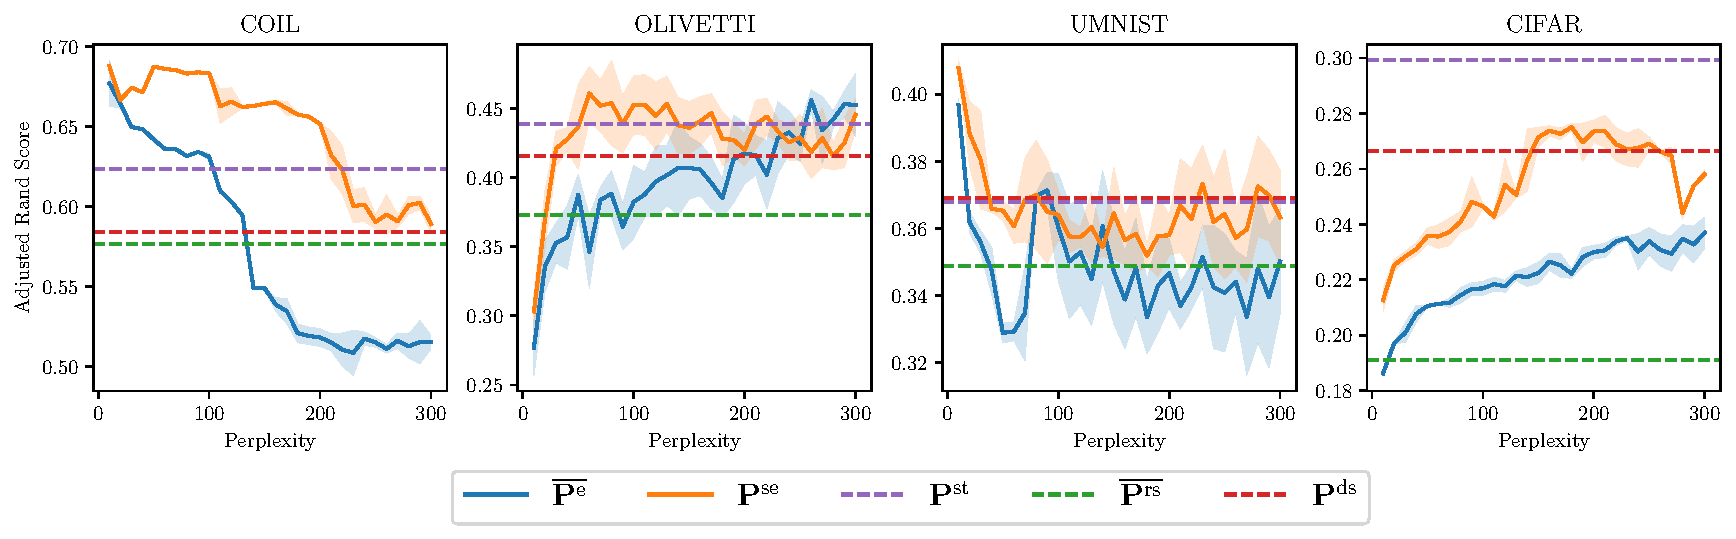
\includegraphics[width=\columnwidth]{figures/SNEkhorn/spectral_clustering_sensitivity.pdf}}
    \caption{ARI spectral clustering score as a function of the perplexity parameter for image datasets.}
    \label{fig:spectral_clustering_sensibility}
    \end{center}
    \vspace{-1.1cm}
\end{figure*}

\paragraph{Spectral Clustering.}
Building on the strong connections between spectral clustering mechanisms and t-SNE
\cite{van2022probabilistic,linderman2019clustering} we first consider spectral
clustering tasks to evaluate the affinity matrix $\Pb^{\mathrm{se}}$
\eqref{eq:sym_entropic_affinity} and compare it against
$\overline{\Pb^{\mathrm{e}}}$ \eqref{symmetrization_tsne}. We also consider two
versions of the Gaussian affinity with scalar bandwidth $\K = \exp(-\C/\nu)$:
the symmetrized row-stochastic $\overline{\Pb^{\mathrm{rs}}} =
\operatorname{Proj}^{\ell_2}_{\mathcal{S}}(\Pb^{\mathrm{rs}})$ where
$\Pb^{\mathrm{rs}}$ is $\K$ normalized by row and $\Pb^{\mathrm{ds}}$
\eqref{eq:plan_sym_sinkhorn}. We also consider the adaptive Self-Tuning
$\Pb^{\mathrm{st}}$ affinity from \cite{zelnik2004self} which relies on an
adaptive bandwidth corresponding to the distance from the $k$-th nearest
neighbor of each point. We use the spectral clustering implementation of
\texttt{scikit-learn} \cite{scikit-learn} with default parameters which uses the
unnormalized graph Laplacian. We measure the quality of clustering using the
Adjusted Rand Index (ARI). Looking at both \cref{table_spectral_microaray} and
\cref{fig:spectral_clustering_sensibility}, one can notice that, in general,
symmetric entropic affinities yield better results than usual entropic
affinities with significant improvements in some datasets (\eg throat microarray
and SNAREseq). Overall $\Pb^{\mathrm{se}}$ outperforms all the other affinities
in $8$ out of $12$ datasets. This shows that the adaptivity of EAs is crucial.
\cref{fig:spectral_clustering_sensibility} also shows that this
superiority is verified for the whole range of perplexities. This can be
attributed to the fact that symmetric entropic affinities combine the advantages
of doubly stochastic normalization in terms of clustering and of EAs in terms of
adaptivity. In the next experiment, we show that these advantages translate into
better clustering and neighborhood retrieval at the embedding level when running
SNEkhorn.

\begin{wrapfigure}[12]{R}{0.5\textwidth}
    \centerline{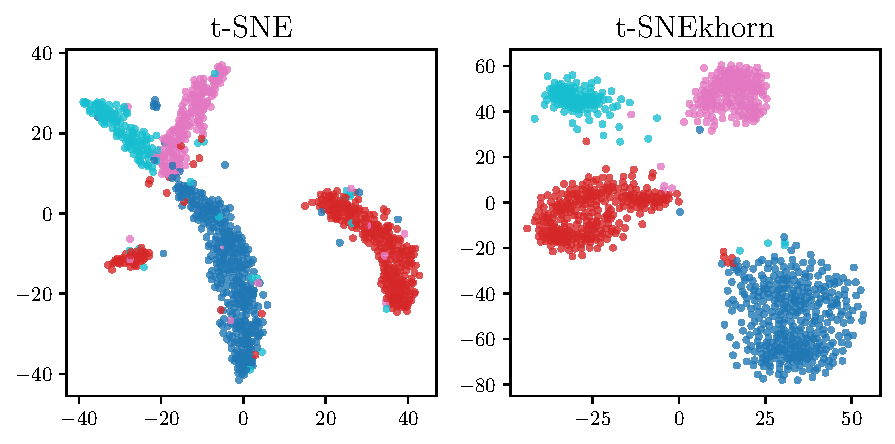
\includegraphics[width=\linewidth]{figures/SNEkhorn/fig_sc.pdf}}
    \captionof{figure}{SNAREseq embeddings produced by t-SNE and t-SNEkhorn with $\xi=50$.}
    \label{fig:sc}
\end{wrapfigure}

\paragraph{Dimension Reduction.}
To guarantee a fair comparison, we implemented not only SNEkhorn, but also t-SNE and UMAP in \texttt{PyTorch} \cite{paszke2017automatic}. 
% Note that UMAP also relies on adaptive affinities but sets the degree of each node (related to the hyperparameter \texttt{n\textunderscore neighbors} which plays a similar role to the perplexity) rather than the entropy.
% Our code is made available with this submission. 
All models were optimized using \texttt{ADAM} \cite{kingma2014adam} with default parameters and the same stopping criterion: the algorithm stops whenever the relative variation of the loss becomes smaller than $10^{-5}$. For each run, we draw independent $\mathcal{N}(0,1)$ coordinates and use this same matrix to initialize all the methods that we wish to compare. To evaluate the embeddings' quality, we make use of the silhouette \cite{rousseeuw1987silhouettes} and trustworthiness \cite{venna2001neighborhood} scores from \texttt{scikit-learn} \cite{scikit-learn} with default parameters.  While the former relies on class labels, the latter measures the agreement between the neighborhoods in input and output spaces, thus giving two complementary metrics to properly evaluate the embeddings. 
The results, presented in \cref{tab:DR_genomics_data}, demonstrate the notable superiority of t-SNEkhorn compared to the commonly used t-SNE and UMAP algorithms. Across the $16$ datasets examined, t-SNEkhorn almost consistently outperformed the others, achieving the highest silhouette score on $15$ datasets and the highest trustworthiness score on $12$ datasets. To visually assess the quality of the embeddings, we provide SNAREseq embeddings in \cref{fig:sc}. Notably, one can notice that the use of t-SNEkhorn results in improved class separation compared to t-SNE.
 
% \begin{table}[h]
% \caption{Silhouette scores ($\times 100$) for the datasets with most samples of the CuMiDa repository.}
% \label{tab:results_microarray}
% \vskip 0.1in
% \begin{center}
% \begin{small}
% \begin{sc}
% \begin{tabular}{lcccccc}
% \toprule
% Data set & t-SNE & UMAP & t-SNEkhor & t-SNE & UMAP & t-SNEkhornn \\
% \midrule
% Liver & 46.1$\pm$ 3.9 & 41.5$\pm$ 7.5& \textbf{58.5$\pm$ 1.0} & 46.1$\pm$ 3.9 & 41.5$\pm$ 7.5& \textbf{58.5$\pm$ 1.0} \\
% Breast & 24.0$\pm$ 5.6 & 21.8$\pm$ 9.6& \textbf{29.4$\pm$ 0.7} \\
% Leukemia & 14.6$\pm$ 5.1 & 9.1$\pm$ 7.4& \textbf{21.1$\pm$ 4.5} \\
% Colorectal & 61.1$\pm$ 2.4 & 58.5$\pm$ 7.7& \textbf{68.3$\pm$ 0.4} \\
% Liver \small{2} & 36.4$\pm$ 1.6 & 26.7$\pm$ 10& \textbf{45.8$\pm$ 0.9} \\
% Breast \small{2} & 26.5$\pm$ 3.2 & \textbf{32.2$\pm$ 2.7} & 30.7$\pm$ 3.8 \\
% Renal & 39.9$\pm$ 1.4 & \textbf{43.2$\pm$ 1.5} & 42.8$\pm$ 0.4 \\
% Brain & 11.1$\pm$ 5.3 & 7.6$\pm$ 7.2 & \textbf{16.3$\pm$ 4.3} \\
% \bottomrule
% \end{tabular}
% \end{sc}
% \end{small}
% \end{center}
% \vskip -0.1in
% \end{table}

\begin{table*}\centering
\caption{Scores for the UMAP, t-SNE and t-SNEkhorn embeddings.}
\vskip 0.1in
\begin{small}
\begin{tabular}{@{\hskip 0.1in}l@{\hskip 0.1in}c@{\hskip 0.1in}c@{\hskip 0.1in}c@{\hskip 0.1in}c@{\hskip 0.1in}c@{\hskip 0.1in}c@{\hskip 0.1in}c@{\hskip 0.1in}c@{\hskip 0.1in}}
    \toprule[1.5pt]
& \multicolumn{3}{c}{Silhouette ($\times 100$)} & & \multicolumn{3}{c}{Trustworthiness ($\times 100$)} \\
\cmidrule{2-4} \cmidrule{6-8}
& UMAP & t-SNE & t-SNEkhorn && UMAP & t-SNE & t-SNEkhorn \\ \midrule
COIL & $20.4\pm3.3$ & $30.7\pm6.9$ & $\mathbf{52.3\pm1.1}$ && $99.6\pm0.1$ & $99.6\pm0.1$ & $\mathbf{99.9\pm0.1}$ \\ 
OLIVETTI & $6.4\pm4.2$ & $4.5\pm3.1$ & $\mathbf{15.7\pm2.2}$ && $96.5\pm1.3$ & $96.2\pm0.6$ & $\mathbf{98.0\pm0.4}$ \\
UMNIST & $-1.4\pm2.7$ & $-0.2\pm1.5$ & $\mathbf{25.4\pm4.9}$ && $93.0\pm0.4$ & $99.6\pm0.2$ & $\mathbf{99.8\pm0.1}$ \\
CIFAR & $13.6\pm2.4$ & $18.3\pm0.8$ & $\mathbf{31.5\pm1.3}$ && $90.2\pm0.8$ & $90.1\pm0.4$ & $\mathbf{92.4\pm0.3}$ \\ \midrule[0.2pt]
Liver \tiny{(14520)} & $49.7\pm1.3$ & $50.9\pm0.7$ & $\mathbf{61.1\pm0.3}$ && $89.2\pm0.7$ & $90.4\pm0.4$ & $\mathbf{92.3\pm0.3}$ \\
Breast \tiny{(70947)} & $28.6\pm0.8$ & $29.0\pm0.2$ & $\mathbf{31.2\pm0.2}$ && $90.9\pm0.5$ & $91.3\pm0.3$ & $\mathbf{93.2\pm0.4}$ \\
Leukemia \tiny{(28497)} & $22.3\pm0.7$ & $20.6\pm0.7$ & $\mathbf{26.2\pm2.3}$ && $90.4\pm1.1$ & $92.3\pm0.8$ & $\mathbf{94.3\pm0.5}$ \\
Colorectal \tiny{(44076)} & $67.6\pm2.2$ & $69.5\pm0.5$ & $\mathbf{74.8\pm0.4}$ && $93.2\pm0.7$ & $93.7\pm0.5$ & $\mathbf{94.3\pm0.6}$ \\
Liver \tiny{(76427)} & $39.4\pm4.3$ & $38.3\pm0.9$ & $\mathbf{51.2\pm2.5}$ && $85.9\pm0.4$ & $89.4\pm1.0$ & $\mathbf{92.0\pm1.0}$ \\
Breast \tiny{(45827)} & $35.4\pm3.3$ & $39.5\pm1.9$ & $\mathbf{44.4\pm0.5}$ && $93.2\pm0.4$ & $94.3\pm0.2$ & $\mathbf{94.7\pm0.3}$ \\
Colorectal \tiny{(21510)} & $38.0\pm1.3$ & $\mathbf{42.3\pm0.6}$ & $35.1\pm2.1$ && $85.6\pm0.7$ & $\mathbf{88.3\pm0.9}$ & $88.2\pm0.7$ \\
Renal \tiny{(53757)} & $44.4\pm1.5$ & $45.9\pm0.3$ & $\mathbf{47.8\pm0.1}$ && $93.9\pm0.2$ & $\mathbf{94.6\pm0.2}$ & $94.0\pm0.2$ \\ 
Prostate \tiny{(6919)} & $5.4\pm2.7$ & $8.1\pm0.2$ & $\mathbf{9.1\pm0.1}$ && $77.6\pm1.8$ & $\mathbf{80.6\pm0.2}$ & $73.1\pm0.5$ \\ 
Throat \tiny{(42743)} & $26.7\pm2.4$ & $28.0\pm0.3$ & $\mathbf{32.3\pm0.1}$ && $\mathbf{91.5\pm1.3}$ & $88.6\pm0.8$ & $86.8\pm1.0$ \\ \midrule[0.2pt]
scGEM & $26.9\pm3.7$ & $33.0\pm1.1$ & $\mathbf{39.3\pm0.7}$ && $95.0\pm1.3$ & $96.2\pm0.6$ & $\mathbf{96.8\pm0.3}$ \\
SNAREseq & $6.8\pm6.0$ & $35.8\pm5.2$ & $\mathbf{67.9\pm1.2}$ && $93.1\pm2.8$ & $99.1\pm0.1$ & $\mathbf{99.2\pm0.1}$ \\
\bottomrule[1.5pt]
\label{tab:DR_genomics_data}
\end{tabular}
\end{small}
\vspace*{-0.5cm}
\end{table*}


% \begin{table*}\centering
%     \ra{1.3}
%     \caption{Scores for the SNE, \texttt{DOSNES} and SNEkhorn embeddings on the images datasets.}
%     \vskip 0.1in
%     \begin{small}
%     \begin{tabular}{@{}lccccccc@{}}\toprule
%     & \multicolumn{3}{c}{Silhouette score ($\times 100$)} & & \multicolumn{3}{c}{Trustworthiness ($\times 100$)} \\
%     \cmidrule{2-4} \cmidrule{6-8}
%     & SNE & \texttt{DOSNES} & SNEkhorn && SNE & \texttt{DOSNES} & SNEkhorn \\ \midrule
%     COIL & 32.5$\pm$1.5 & & \textbf{37.6$\pm$3.2} && 98.1$\pm$0.4 & & \textbf{98.4$\pm$0.1} \\
%     OLIVETTI & 4.5$\pm$3.1 & & \textbf{15.7$\pm$2.2} && 96.2$\pm$0.6 & & \textbf{98.0$\pm$0.4} \\
%     UMNIST & & & && & & \\
%     CIFAR & & & && & & \\
%     \bottomrule
%     \label{tab:DR_genomics_data}
%     \end{tabular}
%     \end{small}
% \end{table*}
    
% !TeX root = ../workshop_paper.tex

\section{Optimal Transport with Adaptive Regularization}\label{sec:OTARI}

In this section, we develop a new formulation of OT, called OT with Adaptive Regularization (OTARI), allowing to control, for any strictly convex function $\psi$, the value of $\psi$ on each row and/or column of the OT plan. 
We then show the advantages of OTARI over usual regularized OT on domain adaptation tasks, focusing particularly on the negative entropy and the $\ell_2$ norm respectively associated with entropic \citep{cuturi2013sinkhorn} and quadratic \citep{blondel2018smooth} optimal transport.

\paragraph{Motivations.}
As discussed in \Cref{sec:background_ot}, regularizing optimal transport (OT) with a strictly convex term is a widely adopted approach that reduces numerical complexity and results in more diffuse OT plans \citep{peyre2019computational}. A prominent example is entropic regularization \citep{cuturi2013sinkhorn}, which produces dense transport plans.

In some applications, the smoothing effect introduced by regularization is of primary importance. A key example, beyond constructing doubly stochastic affinity matrices for clustering and dimensionality reduction, where smoothing helps connect neighboring points (\Cref{sec:doubly_sto} and \Cref{subsec:sea}), is domain adaptation \citep{courty2017joint}, where regularized OT often improves performance compared to non-regularized alternatives (see, for example, \Cref{tab:da_exps}).

Many OT regularization schemes on the primal formulation impose a scalar constraint on the global transport plan.
Consequently, central data points tend to exhibit a denser (or more diffuse) transport plan compared to extreme (or outlier) data points, for which diffusion is more costly. As a result, the latter points receive limited benefits from the smoothing effect introduced by the regularizer as shown in the left side of \cref{fig:entropic_ot_plans}. This partly explains OT's significant sensitivity to outliers in many applications \citep{mukherjee2021outlier, pmlr-v202-chuang23a}.
To remedy this, one needs to constrain the transport plan in a pointwise manner, as we did in the previous sections of this chapter.


\subsection{Formulation of the Problem}\label{sec:pwot}

In this section, we present a new formulation of OT that imposes constraints on each row of the OT plan.
We begin by introducing the set of matrices with \emph{point-wise} constraints. To set the upper bound, we rely again on the perplexity parameter $\xi$ that can be interpreted as the number of effective neighbors for each point. Concretely, we define $\mathbf{e}_{\xi} = \frac{1}{\xi}(\ind_{i \leq \xi})_{i}$ the probability vector of $\xi$ uniform arms and
\begin{align}
  \mathcal{H}_\psi(\xi) &\coloneqq \{\mP \bm{\geq} \bm{0} \: \text{s.t.}\ \: \forall i, \: \psi(\mP_{i:}) \leq \psi(\mathbf{e}_{\xi}) \} \:.
\end{align}
Note that in particular $\psi_{\KL}(\mathbf{e}_{\xi}) = - (\log \xi + 1)$ and $\psi_2(\mathbf{e}_{\xi}) = 1/\xi$.
% In contrast to the constraint utilized in standard strictly convex OT \eqref{eq:scOT}, $\mathcal{H}_\psi(\xi)$ imposes a constraint on \emph{each row} of the transport plan $\mP$.
We now define Optimal Transport with Adaptive Regularization (OTARI) as the generalization of \eqref{eq:cot} to the case where the strictly convex constraint is given by $\mathcal{H}_\psi(\xi)$. Similarly to \Cref{prop:cot}, we can frame OTARI as a $\psi$-Bregman projection of $\mK_\sigma = \nabla \psi^*(-\mC / \sigma)$ or solve it using dual ascent.

\paragraph{OTARI problem.}
  Let $(\bm{a}, \bm{b}, \xi)$ be such that $\gU(\bm{a}, \bm{b}) \cap \mathcal{H}_\psi(\xi)$ has an interior point.
  We consider the following problem:
  \begin{align}\label{eq:pcOT}
    \min_{\mP \in \gU(\bm{a}, \bm{b})} \: \langle \mP, \mC \rangle \quad \text{s.t.} \quad  \mP \in \mathcal{H}_\psi(\xi) \:.
    \tag{OTARI-s}
\end{align}

% \begin{table}[h]
%   \centering
%   \caption{Table caption}
%   \label{tab:example}
%   \begin{tabular}{lccc}
%     \toprule
%     & $\psi(\mathbf{p})$ & $\nabla \psi(\mathbf{p})$ & $\nabla \psi^\star(\mathbf{p})$ \\
%     \midrule
%     Negative entropy & $\langle \mathbf{p}, \log \mathbf{p} - 1 \rangle$ & $\log(\mathbf{p})$ & $\exp(\mathbf{p})$ \\
%     $\alpha$ norm & $\frac{1}{\alpha} \| \mathbf{p} \|_{\alpha}^{\alpha}$ & $\vp^{\odot (\alpha-1)}$ & $\frac{1}{\alpha} [\vp]_{+}^{\odot 1 / (\alpha-1)}$ \\
%     $\alpha$ norm with sparsity constraint & $\frac{1}{\alpha} \| \mathbf{p} \|_{\alpha}^{\alpha} + \delta_{k}(\vp)$ & & $\frac{1}{\alpha} \sum_{i \in \integ{k}} [p_i]_{+}^{1 / (\alpha-1)}$ \\
%     \bottomrule
%   \end{tabular}
%   \vspace{0.5cm}
% \end{table}


\begin{proposition}\label{prop:pcot}
  Let $(\bm{a}, \bm{b}, \xi)$ be such that $\gU(\bm{a}, \bm{b}) \cap \mathcal{H}_\psi(\xi)$ has an interior point and let $\mP^\star$ solve
  \begin{align}\label{eq:pcOT}
    \min_{\mP \in \gU(\bm{a}, \bm{b})} \: \langle \mP, \C \rangle \quad \text{s.t.} \quad  \mP \in \mathcal{H}_\psi(\xi) \:.
    \tag{OTARI-s}
\end{align}
Let $\bm{\varepsilon}^\star$ be the optimal dual variable associated with the constraint $\mP \in \mathcal{H}_\psi(\xi)$.
If $\bm{\varepsilon}^\star \bm{>} \bm{0}$, then it holds $\mP^\star = \operatorname{Proj}^{D_\psi}_{\gU(\bm{a}, \bm{b}) \cap \mathcal{H}_\psi(\xi)}(\mK_\sigma)$ for any $0 < \sigma \leq \min_i{\varepsilon_i^\star}$. Moreover it holds $\mP^\star = \nabla \psi^* \left(\diag(\bm{\varepsilon}^\star)^{-1} (\mC - \bm{\lambda}^\star \oplus \bm{\mu}^\star) \right)$ where $(\bm{\lambda}^\star, \bm{\mu}^\star, \bm{\varepsilon}^\star)$ solve the following dual
\begin{align}
  \max_{\bm{\lambda}, \bm{\mu}, \bm{\varepsilon} \bm{>} \bm{0}} \: \langle \bm{\lambda}, \bm{a} \rangle + \langle \bm{\mu}, \bm{b} \rangle + \left\langle \bm{\varepsilon}, \psi^*\left(\diag(\bm{\varepsilon})^{-1} (\mC - \bm{\lambda} \oplus \bm{\mu}) \right) - \psi(\mathbf{e}_\xi) \bm{1}  \right\rangle \:.
  \tag{Dual-OTARI-s}
\end{align}
\end{proposition}

\begin{figure*}[t]
  \begin{center}
  \centerline{\includegraphics[width=\columnwidth]{figures/OTARI/visu_entropic_OTARI.pdf}}
  \caption{Entropic OT plans ($\xi=5$) with global constraint, pointwise constraints on sources and then on targets. The three plans have the same global entropy. The color of each source (resp. target) point shows the perplexity (exponential of entropy) of the associated row (resp. column) of the OT plan.}
  \label{fig:entropic_ot_plans}
  \end{center}
  % \vspace{-0.5cm}
\end{figure*}

% The doubly constrained problem, referred to as \eqref{eq:dpcOT}, is as follows for two perplexity parameters $\xi^{a}$ and $\xi^{b}$
% \begin{align}\label{eq:dpcOT}
%     \min_{\mP \in \gU(\bm{a}, \bm{b})} \: \langle \mP, \mC \rangle \quad \text{s.t.} \quad  \mP \in \mathcal{B}_\psi(\xi^{a}) \quad \text{and} \quad \mP^\top \in \mathcal{B}_\psi(\xi^{b})
%     \tag{OTARI-d}
%   \end{align}
% and can also be seen as a $\psi$-Bregman projection through a trivial extension of \cref{prop:pcot}. \hug{à reprendre}

% \begin{wrapfigure}[18]{L}{0.52\textwidth}
%   \begin{minipage}{0.52\textwidth}
\begin{algorithm}[H]
  \caption{\textit{Dykstra} for solving (OTARI-d)}
  \label{algo:Dykstra_pcot}
  \begin{algorithmic}[1]
      \STATE {\textbf{Input}: $\mC$, $\psi(\cdot)$, $\xi^{a}$, $\xi^{b}$, $\varepsilon$}, $\bm{a}$, $\bm{b}$ \\
      % \STATE $t \leftarrow 0$ \\
      \STATE $\left(\mP_b, \bm{\Xi}, \bm{\Theta} \right) \leftarrow \left(\nabla \psi^{\star}(-\mC / \varepsilon), \mathbf{0}, \mathbf{0} \right)$ \\
      \WHILE{not converged}
          % \STATE $t \leftarrow t+1$ \\
          \STATE $\mP_a \leftarrow \operatorname{Proj}^{D_\psi}_{\gU(\bm{a})}(\mP_b)$ 
          \\
          \STATE $\overline{\mP}_{a} \leftarrow \operatorname{Proj}^{D_\psi}_{\mathcal{B}_{\psi}(\xi^{a})}\circ \nabla \psi^*(\nabla \psi(\mP_a) + \bm{\Xi})$ 
          \\
          \STATE $\bm{\Xi} \leftarrow \bm{\Xi} + \nabla \psi(\mP_{a}) - \nabla \psi(\overline{\mP}_{a})$
          \\
          \STATE $\mP^\top_b \leftarrow \operatorname{Proj}^{D_\psi}_{\Pi(\bm{b})}(\overline{\mP}_{a}^\top)$ 
          \\
          \STATE $\overline{\mP}_{b}^\top \leftarrow \operatorname{Proj}^{D_\psi}_{\mathcal{B}_{\psi}(\xi^{b})}\circ \nabla \psi^*((\nabla \psi(\mP_b) + \bm{\Theta})^\top)$ 
          \\
          \STATE $\bm{\Theta} \leftarrow \bm{\Theta} + \nabla \psi(\mP_{b}) - \nabla \psi(\overline{\mP}_{b})$
      \ENDWHILE  
      \STATE {\bfseries Output: $\overline{\mP}_{b}$}
\end{algorithmic}
\end{algorithm}
% \end{minipage}
% \end{wrapfigure}

According to \cref{prop:pcot}, one can solve \eqref{eq:pcOT} using either alternating projections or dual ascent. 
% Note that upon convergence, dual ascent outputs the exact solution of \eqref{eq:pcOT} as it provides a set of variables $(\mP^\star, \bm{\lambda}^\star, \bm{\mu}^\star, \bm{\varepsilon}^\star)$ satisfying its KKT conditions. 
When $\bm{\varepsilon}^\star \bm{>} \bm{0}$, meaning that all constraints are active \ie $\forall i, \: \psi(\mP^\star_{i:}) = \psi(\mathbf{p}_{\xi})$, dual ascent is usually faster. However, if $\bm{\varepsilon}^\star$ has null components, one can still rely on $\operatorname{Proj}^{D_\psi}_{\gU(\bm{a}, \bm{b}) \cap \mathcal{H}_\psi(\xi)}(\mK_\varepsilon)$ to provide an approximate solution as alternating Bregman projections are always guaranteed to converge.

Note that we can impose the pointwise constraint equivalently on the rows or the columns of the OT plan. Hence (OTARI-t) can be defined by imposing the constraint on the target samples \textit{i.e.}\ $\mP^\top \in \mathcal{H}_\psi(\xi)$.
We also propose a doubly constrained formulation called (OTARI-d) that consists of projecting $\mK_\sigma$ onto the nonempty set $\mathcal{B}_\psi(\xi^{a}) \cap \mathcal{B}^\top_\psi(\xi^b)$ 
% where $\xi^{a}$ and $\xi^{b}$ are chosen such that this intersection is nonempty 
where we defined $\mathcal{B}^\top_\psi(\xi) = \{ \mP^\top \in \mathcal{H}_\psi(\xi)\}$ thus ensuring sufficient smoothing for both rows and columns.
Such projection can be computed using alternating Bregman projections, whose convergence has been well-studied \citep{censor1998dykstra, benamou2015iterative}.
As we generally do not have access to a closed form for the projection onto the transport polytope $\gU(\bm{a}, \bm{b})$, it is common to alternate projection onto $\gU(\bm{a})$ and $\Pi(\bm{b})$ separately (see \eg the seminal Sinkhorn algorithm \citep{cuturi2013sinkhorn}).
We extend this scheme by adding projection steps into the pointwise constraints $\mathcal{H}_\psi(\xi)$ for both $\mP$ and $\mP^\top$. As this set is not affine, one needs to resort to the Dykstra procedure \citep{dykstra1983algorithm} that can be applied to a broad class of Bregman divergences \citep{bauschke2000dykstras}, as shown in \cref{algo:Dykstra_pcot}.
% It consists of adding corrective terms to the non-affine projection. 
In \cref{sec:proof_projs}, we provide the form of the projections for $\psi_{\KL}$ and $\psi_2$. A key benefit of decoupling both row and column constraints is that projection onto $\mathcal{B}_{\psi}(\xi)$ exhibits a simple structure where the rows can be decoupled into independent subproblems.
% In the latter, $\psi^*$ is the Fenchel conjugate of $\psi$.


\subsubsection{Application to Domain Adaptation}

\begin{figure}[h]
  \begin{center}
  \centerline{\includegraphics[width=\columnwidth]{figures/OTARI/visu_DA.pdf}}
  \caption{Toy domain adaptation scenario with entropic OT plans ($\xi=10$) with various constraints. The size of the point is proportional to the associated entropy. When using Sinkhorn, barycentric mapping match outliers points since the OT plan is less diffuse for these points. In turn, using pointwise constraints concentrate the 
   mapped points in high-density regions, thus giving more robust estimates for the mappings onto the target domain.}
  \label{fig:visu_DA}
  \end{center}
\end{figure}

\begin{table}[h]
  % \begin{wraptable}[7]{L}{8.5cm}
    % \vspace*{-0.4cm}
    \centering
    % Note that unregularized OT does not depend on $\xi$. }
    \begin{small}
    \begin{tabular}{lc@{\hskip 0.1in}c@{\hskip 0.1in}c@{\hskip 0.1in}c@{\hskip 0.1in}c@{\hskip 0.1in}c}
    \toprule[1.5pt]
    & OT& EOT & EOTARI-s & EOTARI-t & EOTARI-d \\
    \midrule
    MNIST $\to$ USPS ($\xi=30$) & $53.1(5.4)$ & $64.2(2.8)$ & $65.0(5.3)$ & $66.4(3.5)$ & $\mathbf{67.4(2.9)}$ \\
    MNIST $\to$ USPS ($\xi=300$) & $53.1(5.4)$ & $68.8(3.1)$ & $70.8(4.2)$ & $70.2(3.4)$ & $\mathbf{72.6(5.1)}$ \\
  
    USPS $\to$ MNIST ($\xi=30$) & $59.1(4.9)$ & $60.8(5.4)$ & $61.6(4.4)$ & $\mathbf{62.6(3.0)}$ & $61.0(4.7)$ \\
    USPS $\to$ MNIST ($\xi=300$) & $59.1(4.9)$ & $59.8(1.6)$ & $61.0(2.3)$ & $\mathbf{61.6(3.0)}$ & $58.8(2.3)$ \\
    \midrule
    \midrule
    & OT & QOT & QOTARI-s & QOTARI-t & QOTARI-d \\
    \midrule
    MNIST $\to$ USPS ($\xi=30$) & $53.1(5.4)$ & $68.3(3.9)$ & $68.3(3.6)$ & $\mathbf{69.3(4.7)}$ & $68.1(4.6)$ \\
    MNIST $\to$ USPS ($\xi=300$) & $53.1(5.4)$ & $60.7(1.5)$ & $\mathbf{67.0(2.4)}$ & $65.5(2.3)$ & $65.8(2.5)$ \\
    USPS $\to$ MNIST ($\xi=30$) & $59.1(4.9)$ & $60.4(3.5)$ & $\mathbf{62.8(3.7)}$ & $59.6(2.7)$ & $61.6(3.1)$ \\
    USPS $\to$ MNIST ($\xi=300$) & $59.1(4.9)$ & $59.2(3.4)$ & $60.1(3.0)$ & $\mathbf{62.0(3.7)}$ & $61.5(3.8)$ \\
    \bottomrule[1.5pt]
    \end{tabular}
    \end{small}
    \vspace{0.4cm}
    \caption{Domain adaptation 1-NN classification scores for OT (unregularized), EOT (entropic), EOTARI (entropic OTARI), QOT (quadratic), QOTARI (quadratic OTARI) for $\xi=30$ and $\xi=300$.}
    \label{tab:da_exps}
    \vspace{0.1cm}
  \end{table}

In this section, we evaluate OTARI on a domain adaptation task where the goal is to transport labeled data points to a target domain where a classifier is trained. Mapping onto the target domain is performed through a barycentric mapping of the form: for any $i \in \integ{N_S}$, $\hat{\bm{x}}_i = \frac{1}{a_i} \sum_j T_{ij} \bm{x}_j^T$.
Looking at \cref{fig:visu_DA}, one can notice that using OTARI for domain adaptation yields a mapping that is concentrated in high-density (thus more faithful) regions of the target domain. On the opposite, when using globally constrained OT (left side of \cref{fig:visu_DA}), the barycentric mapping associated with an outlier is concentrated on the outlier's position. For the experiments, we take $\C$ as the squared Euclidean distance computed from raw images of the handwritten digit classification benchmark MNIST-USPS. 
Following the standard practice in OT-based domain adaptation \citep{flamary2016optimal}, we map the source to the target samples and then train a 1-NN classifier on the barycentric mappings with source labels.
We compute the outcomes across 10 independent trials. In each of these experiments, the target data is partitioned into a 90\% training and 10\% testing split, with OT barycentric mappings and 1-NN classifiers exclusively applied to the training set. Mean scores and standard deviations are displayed in \cref{tab:da_exps}. The latter shows that adaptive regularization consistently outperforms global regularization (set such that $\sum_i \psi(\mP^\star_{i:}) = n \psi(\mathbf{e}_{\xi})$ where $\mP^\star$ solves \ref{eq:cot} for a fair comparison) with significant performance gains in some settings.

\paragraph{Possible extensions.}
Among possible extensions of \Cref{eq:pcOT}, one could also extend OTARI to continuous distributions and apply it to OT mapping estimation \citep{pooladian2021entropic}. Other interesting directions include
investigating optimization algorithms that can avoid quadratic memory complexity.

%!TEX root = ../paper.tex 

\section{Proofs}\label{sec:proofs}

% \subsection{Euclidean Projection onto $\mathcal{S}$}\label{sec:sym_proj}

% % \paragraph{Euclidean projection onto $\mathcal{S}$.}
% It amounts to the following problem.
% \begin{align}
%     \argmin_{\Pb \in \mathcal{S}} \: &\| \Pb - \K \|_2^2 \:.
% \end{align}
% With $\W \in \R^{n \times n}$, the Lagrangian takes the form: 
% \begin{equation}
% \mathcal{L}(\Pb, \W) = \| \Pb - \K \|_2^2 +\langle \W, \Pb -\Pb^{\top} \rangle \:.
% \end{equation}
% Cancelling the gradient of $\mathcal{L}$ with respect to $\Pb$ gives $2(\Pb^\star - \K) + \W - \W^\top = \bm{0}$. Thus $\Pb^\star = \K + \frac{1}{2} \left(\W^\top - \W \right)$. Using the symmetry constraint on $\Pb^\star$ yields $\Pb^\star = \frac{1}{2} \left(\K + \K^\top \right)$.
% Hence we have:
% \begin{equation}
% \argmin_{\Pb \in \mathcal{S}} \: \| \Pb -  \K \|_2^2 = \frac{1}{2} \left(\K + \K^\top \right) \:.
% \end{equation}

% \subsection{From Symmetric Entropy-Constrained OT to Sinkhorn Iterations}\label{sec:proof_sinkhorn}

% In this section, we derive Sinkhorn iterations from the problem (\ref{eq:entropy_constrained_OT}). Let $\C \in \mathcal{D}$. We start by making the constraints explicit.
% \begin{align}
%     \min_{\Pb \in \R_+^{n \times n}} \quad &\langle \Pb, \C \rangle \\
%     \text{s.t.} \quad &\sum_{i \in \integ{n}} \operatorname{H}(\Pb_{i:}) \geq \eta \\
%     & \Pb \bm{1} = \bm{1}, \quad \Pb = \Pb^\top \:.
% \end{align}
% For the above convex problem the Lagrangian writes, where $\nu \in \mathbb{R}_+$, $\mathbf{f} \in \mathbb{R}^n$ and $\bm{\Gamma} \in \mathbb{R}^{n \times n}$:
% \begin{align}
%     \mathcal{L}(\Pb, \mathbf{f}, \nu, \bm{\Gamma}) &= \langle \Pb, \C \rangle + \Big\langle \nu, \eta - \sum_{i \in \integ{n}} \operatorname{H}(\Pb_i) \Big\rangle + 2\langle \mathbf{f}, \bm{1} - \Pb \bm{1} \rangle + \big\langle \bm{\Gamma}, \Pb - \Pb^\top \big\rangle \:.
% \end{align}
% Strong duality holds and the first order KKT condition gives for the optimal primal $\Pb^\star$ and dual $(\nu^\star, \mathbf{f}^\star, \bm{\Gamma}^\star)$ variables: 
% \begin{align}
%     \nabla_{\Pb} \mathcal{L}(\Pb^\star, \mathbf{f}^\star, \nu^\star, \bm{\Gamma}^\star) &= \C + \nu^\star \log{\Pb^\star} - 2\mathbf{f}^\star \bm{1}^\top + \bm{\Gamma}^\star - \bm{\Gamma}^{\star\top} = \bm{0} \:.
% \end{align}
% Since $\Pb^\star, \C \in \mathcal{S}$ we have $\bm{\Gamma}^\star - \bm{\Gamma}^{\star\top} = \mathbf{f}^\star \bm{1}^\top - \bm{1}\mathbf{f}^{\star \top}$. Hence $\C + \nu^\star \log{\Pb^\star} - \mathbf{f}^\star \oplus \mathbf{f}^\star = \bm{0}$. Suppose that $\nu^\star = 0$ then the previous reasoning implies that $\forall (i,j), C_{ij} = f_i^\star + f_j^\star$. Using that $\C \in \mathcal{D}$ we have $C_{ii} = C_{jj} = 0$ thus $\forall i,  f^\star_i = 0$ and thus this would imply that $\C = 0$ which is not allowed by hypothesis. Therefore $\nu^\star \neq 0$ and the entropy constraint is saturated at the optimum by complementary slackness. Isolating $\Pb^\star$ then yields:
% \begin{align}
%     \Pb^{\star} &= \exp{\left( (\mathbf{f}^\star \oplus \mathbf{f}^{\star} - \C) / \nu^\star \right)} \:.
% \end{align}
% $\Pb^\star$ must be primal feasible in particular $\Pb^\star \bm{1} = \bm{1}$. This constraint gives us the Sinkhorn fixed point relation for $\mathbf{f}^\star$:
% \begin{align}
%     \forall i \in \integ{n}, \quad [\mathbf{f}^\star]_i = - \nu^\star \operatorname{LSE} \big((\mathbf{f}^\star - \C_{:i}) / \nu^\star \big)\,,
% \end{align}
% where for a vector $\bm{\alpha}$, we use the notation
% $\operatorname{LSE}(\bm{\alpha}) = \log \sum_{k} \exp (\alpha_k)$.



\subsection{Proof of \cref{prop:entropic_affinity_as_linear_program}}

\entropicaffinityaslinearprogram*

\begin{proof}
We begin by rewriting the above problem to make the constraints more explicit.
\begin{align*}
    \min_{\Pb \in \R_+^{n \times n}} \quad &\langle \Pb, \C \rangle \\
    \text{s.t.} \quad &\forall i, \: \operatorname{H}(\Pb_{i:}) \geq \log{\xi} + 1 \\
    & \Pb \bm{1} = \bm{1} \:.
\end{align*}
By concavity of entropy, one has that the entropy constraint is convex thus the above primal problem is a convex optimization problem. Moreover, the latter is strictly feasible for any $\xi \in \integ{n-1}$. Therefore Slater's condition is satisfied and strong duality holds.

Introducing the dual variables $\bm{\lambda} \in \mathbb{R}^n$ and $\bm{\varepsilon} \in \mathbb{R}_+^n$, the Lagrangian of the above problem writes:
\begin{align}
    \mathcal{L}(\Pb, \bm{\lambda}, \bm{\varepsilon}) &= \langle \Pb, \C \rangle + \langle \bm{\varepsilon}, (\log{\xi}+1) \bm{1} - \operatorname{H}_{\mathrm{r}}(\Pb) \rangle + \langle \bm{\lambda}, \bm{1} - \Pb \bm{1} \rangle\,,
\end{align}
where we recall that $\operatorname{H}_{\mathrm{r}}(\Pb) = \left( \operatorname{H}(\Pb_{i:}) \right)_{i}$. Note that we will deal with the constraint $\Pb \in \R_+^{n \times n}$ directly, hence there is no associated dual variable. Since strong duality holds, for any solution $\Pb^\star$ to the primal problem and any solution $(\bm{\varepsilon}^\star, \bm{\lambda}^\star)$ to the dual problem, the pair $\Pb^\star, (\bm{\varepsilon}^\star, \bm{\lambda}^\star)$ must satisfy the Karush-Kuhn-Tucker (KKT) conditions. The first-order optimality condition gives:
\begin{equation}
\label{kkt_ea}
\tag{first-order}
    \nabla_{\Pb} \mathcal{L}(\Pb^\star, \bm{\varepsilon}^\star, \bm{\lambda}^\star) = \C + \operatorname{diag}(\bm{\varepsilon}^\star)\log{\Pb^\star} - \bm{\lambda}^\star \bm{1}^\top = \bm{0} \:.
\end{equation}
Assume that there exists $\ell \in \integ{n}$ such that $\bm{\varepsilon}_\ell^\star = 0$. Then \Cref{kkt_ea} gives that the $\ell^{th}$ row of $\C$ is constant which is not allowed by hypothesis. Therefore $\bm{\varepsilon}^\star>\bm{0}$ (\ie $\bm{\varepsilon}^\star$ has positive entries). 
Thus isolating $\Pb^\star$ in the first order condition results in:
\begin{align}
    \Pb^\star &= \operatorname{diag}(\mathbf{u}) \exp{(-\operatorname{diag}(\bm{\varepsilon}^\star)^{-1}\C)}
\end{align}
where $\mathbf{u} = \exp{(\bm{\lambda}^\star \oslash \bm{\varepsilon}^\star)}$.
This matrix must satisfy the stochasticity constraint $\Pb \bm{1}=\bm{1}$. Hence one has $\mathbf{u} = \bm{1} \oslash (\exp{(\operatorname{diag}(\bm{\varepsilon}^\star)^{-1}\C)} \bm{1})$ and $\Pb^\star$ has the form
\begin{align}
    \forall (i,j) \in \integ{n}^2, \quad P^{\star}_{ij} = \frac{\exp{(-C_{ij}/\varepsilon^\star_i)}}{\sum_\ell \exp{(-C_{i\ell}/\varepsilon^\star_i)}} \:.
\end{align}
As a consequence of $\bm{\varepsilon}^\star \bm{>} \bm{0}$, complementary slackness in the KKT conditions gives us that for all $i$, the entropy constraint is saturated \ie $\operatorname{H}(\Pb^\star_{i:}) = \log{\xi} + 1$. Therefore $\Pb^\star$ solves the problem \Cref{eq:entropic_affinity_pb}. Conversely any solution of \Cref{eq:entropic_affinity_pb} $P^{\star}_{ij} = \frac{\exp{(-C_{ij}/\varepsilon^\star_i)}}{\sum_\ell \exp{(-C_{i\ell}/\varepsilon^\star_i)}}$ with $(\varepsilon^\star_i)$ such that $\operatorname{H}(\Pb^\star_{i:}) = \log{\xi} + 1$  gives an admissible matrix for $\min_{\Pb \in \mathcal{H}_\xi} \langle \Pb, \C \rangle$ and the associated variables satisfy the KKT conditions which are sufficient conditions for optimality since the problem is convex.
\end{proof}

\subsection{Proof of \cref{prop:saturation_entropies} and \cref{prop:sol_gamma_non_null} \label{proof:main_props}}

The goal of this section is to prove the following results:

\saturation*

\solvingsea*

The unicity of the solution in \cref{prop:saturation_entropies} is a consequence of the following lemma

\begin{lemma} 
\label{lemma:unicity}
  Let $\C \neq 0 \in \mathcal{S}$ with zero diagonal. Then the problem $\min_{\Pb \in \mathcal{H}_{\xi} \cap \mathcal{S}} \: \langle \Pb, \C \rangle$ has a unique solution.
\end{lemma}

\begin{proof}
Making the constraints explicit, the primal problem of symmetric entropic affinity takes the following form
\begin{equation}
\begin{aligned}
    \min_{\Pb \in \R_+^{n \times n}} \quad &\langle \Pb, \C \rangle \\
    \text{s.t.} \quad &\forall i, \: \operatorname{H}(\Pb_{i:}) \geq \log{\xi} + 1 \\
    & \Pb \bm{1} = \bm{1}, \quad \Pb = \Pb^\top \:.
\end{aligned}
\tag{SEA}\label{opt-sym_P}
\end{equation}
Suppose that the solution is not unique \ie there exists a couple of optimal solutions $(\Pb_1, \Pb_2)$ that satisfy the constraints of \eqref{opt-sym_P} and such that $\langle \Pb_1, \C \rangle=\langle \Pb_2, \C \rangle$. For $i \in \integ{n}$, we denote the function $f_{i}: \Pb \rightarrow (\log{\xi} + 1)-\operatorname{H}(\Pb_{i:})$. Then  $f_i$ is continuous, strictly convex and the entropy conditions of  \eqref{opt-sym_P} can be written as $\forall i \in \integ{n}, f_{i}(\Pb) \leq 0$. 

Now consider $\Qb = \frac{1}{2} (\Pb_1 + \Pb_2)$. Then clearly $\Qb \bm{1} = \bm{1}, \Qb = \Qb^\top$. Since $f_i$ is strictly convex we have $f_i(\Qb) = f_i(\frac{1}{2}\Pb_1+\frac{1}{2}\Pb_2) < \frac{1}{2} f_i(\Pb_1) +\frac{1}{2} f(\Pb_2) \leq 0$. Thus $f_i(\Qb) < 0$ for any $i \in \integ{n}$. Take any $\varepsilon >0$ and $i \in \integ{n}$. By continuity of $f_i$ there exists $\delta_i > 0$ such that, for any $\Hb$ with $\|\Hb\|_F \leq \delta_i$, we have $f_{i}(\Qb+\Hb) < f_{i}(\Qb)+ \varepsilon$. Take $\varepsilon >0$ such that $\forall i \in \integ{n},  0 < \varepsilon < -\frac{1}{2} f_{i}(\Qb)$ (this is possible since for any $i \in \integ{n}, f_{i}(\Qb) <0$) and $\Hb$ with $\|\Hb\|_F \leq \min_{i \in \integ{n}} \delta_i$. Then for any $i \in \integ{n}, f_{i}(\Qb+\Hb) < 0$. In other words, we have proven that there exists $\eta > 0$ such that for any $\Hb$ such that $\|\Hb\|_F \leq \eta$, it holds: $\forall i \in \integ{n}, f_i(\Qb+\Hb) < 0$.

Now let us take $\Hb$ as the Laplacian matrix associated to $\C$ \ie for any $(i,j) \in \integ{n}^2$, $H_{ij} = -C_{ij}$ if $i \neq j$ and $\sum_l C_{il}$ otherwise.
Then we have $\langle \Hb, \C \rangle = -\sum_{i \neq j} C_{ij}^2+ 0 = - \sum_{i \neq j} C_{ij}^2 < 0$ since $\C$ has zero diagonal (and is nonzero). Moreover, $\Hb = \Hb^\top$ since $\C$ is symmetric and $\Hb \bm{1} = \bm{0}$ by construction. Consider for $0 < \beta \leq \frac{\eta}{\|\Hb\|_F}$, the matrix $\Hb_{\beta} := \beta \Hb$. Then $\|\Hb_\beta\|_F = \beta \|\Hb\|_F \leq \eta$. By the previous reasoning one has: $\forall i \in \integ{n}, f_i(\Qb+\Hb_{\beta}) < 0$. Moreover, $(\Qb+\Hb_{\beta})^{\top} = \Qb+\Hb_{\beta}$ and $(\Qb+\Hb_{\beta})\bm{1} = \bm{1}$. For $\beta$ small enough we have $\Qb+\Hb_{\beta}\in \R_{+}^{n \times n}$ and thus there is a $\beta$ (that depends on $\Pb_1$ and $\Pb_2$) such that $\Qb+\Hb_{\beta}$ is admissible \ie satisfies the constraints of \eqref{opt-sym_P}. Then, for such $\beta$, 
\begin{equation}
\begin{split}
\langle \C, \Qb+\Hb_{\beta} \rangle- \langle \C, \Pb_1 \rangle &= \frac{1}{2} \langle \C, \Pb_1+ \Pb_2 \rangle + \langle \C, \Hb_{\beta} \rangle -\langle \C, \Pb_1 \rangle\\
&= \langle \C, \Hb_{\beta} \rangle = \beta \langle \Hb, \C \rangle < 0\,.
\end{split}
\end{equation}
Thus $\langle \C, \Qb+\Hb_{\beta} \rangle <\langle \C, \Pb_1 \rangle$ which leads to a contradiction.
\end{proof}
We can now prove the rest of the claims of  \cref{prop:saturation_entropies} and \cref{prop:sol_gamma_non_null}.
\begin{proof}
Let $\C \in \mathcal{D}$. We first prove \cref{prop:saturation_entropies}. The unicity is a consequence of \cref{lemma:unicity}. For the saturation of the entropies we consider the Lagrangian of the problem \eqref{opt-sym_P} that writes $$\mathcal{L}(\Pb, \bm{\lambda}, \bm{\gamma, \bm{\Gamma}}) = \langle \Pb, \C \rangle + \langle \bm{\gamma}, (\log{\xi}+1) \bm{1} - \operatorname{H}_r(\Pb) \rangle + \langle \bm{\lambda}, \bm{1} - \Pb \bm{1} \rangle + \langle \bm{\Gamma}, \Pb - \Pb^\top \rangle$$ for dual variables $\bm{\gamma} \in \mathbb{R}_+^n$, $\bm{\lambda} \in \mathbb{R}^n$ and $\bm{\Gamma} \in \mathbb{R}^{n \times n}$. Strong duality holds by Slater's conditions because $\frac{1}{n} \bm{1} \bm{1}^{\top}$ is stricly feasible for $\xi \leq n-1$. Since strong duality holds, for any solution $\Pb^\star$ to the primal problem and any solution $(\bm{\gamma}^\star, \bm{\lambda}^\star, \bm{\Gamma}^\star)$ to the dual problem, the pair $\Pb^\star, (\bm{\gamma}^\star, \bm{\lambda}^\star, \bm{\Gamma}^\star)$ must satisfy the KKT conditions. They can be stated as follows:
\begin{equation}
    \begin{aligned}
    &\C + \operatorname{diag}(\bm{\gamma}^\star)\log{\Pb^\star} - \bm{\lambda}^\star \bm{1}^\top + \bm{\Gamma}^\star - \bm{\Gamma}^{\star\top} = \bm{0} \\
    &\Pb^\star \bm{1} = \bm{1}, \: \operatorname{H}_r(\Pb^\star) \geq (\log{\xi} + 1)\bm{1}, \: \Pb^\star = \Pb^{\star \top} \\
    &\bm{\gamma}^\star \bm{\geq} \bm{0} \\
    &\forall i, \gamma_i^\star (\operatorname{H}(\Pb_{i:}^\star) - (\log{\xi} + 1)) = 0\:.
\end{aligned}
\tag{KKT-SEA}\label{KKT-sym_P}
\end{equation}
Let us denote $I = \{\ell \in \integ{n} \: \text{s.t.} \: \gamma_\ell^\star = 0\}$. For $\ell \in I$, using the first-order condition, one has for $i \in \integ{n}, C_{\ell i} = \lambda^\star_\ell - \Gamma^\star_{\ell i} + \Gamma^{\star}_{i \ell}$. Since $\C \in \mathcal{D}$, we have $C_{\ell \ell} = 0$ thus $\lambda^\star_\ell = 0$ and $C_{\ell i} = \Gamma^\star_{i \ell} - \Gamma^{\star}_{\ell i}$.
For $(\ell, \ell') \in I^2$, one has $C_{\ell \ell'} = \Gamma^\star_{\ell' \ell} - \Gamma^{\star}_{\ell \ell'} = - (\Gamma^{\star}_{\ell \ell'} - \Gamma^\star_{\ell' \ell}) = - C_{\ell' \ell}$. $\C$ is symmetric thus $C_{\ell \ell'}=0$. Since $\C$ only has null entries on the diagonal, this shows that $\ell = \ell'$ and therefore $I$ has at most one element. By complementary slackness condition (last row of the \ref{KKT-sym_P} conditions) it holds that $\forall i \neq \ell, \operatorname{H}(\Pb^{\star}_{i:}) = \log \xi + 1$. Since the solution of \eqref{opt-sym_P} is unique $\Pb^\star = \Pb^{\mathrm{se}}$ and thus $\forall i \neq \ell, \operatorname{H}(\Pb^{\mathrm{se}}_{i:}) = \log \xi + 1$ which proves \cref{prop:saturation_entropies} but also that for at least $n-1$ indices $\gamma_i^\star > 0$. Moreover, from the KKT conditions we have
\begin{equation}
\forall (i,j) \in \integ{n}^2, \ \Gamma^\star_{ji}-\Gamma^\star_{ij} =  C_{ij}+\gamma^\star_i \log P^\star_{ij}-\lambda^\star_i\,.
\end{equation}
Now take $(i,j) \in \integ{n}^2$ fixed. From the previous equality 
$\Gamma^\star_{ji}-\Gamma^\star_{ij} =  C_{ij}+\gamma^\star_i \log P^\star_{ij}-\lambda^\star_i$ but also $\Gamma^\star_{ij}-\Gamma^\star_{ji} =  C_{ji}+\gamma^\star_j \log P^\star_{ji}-\lambda^\star_j$. Using that $\Pb^\star=(\Pb^{\star})^{\top}$ and $\C \in \mathcal{S}$ we get $\Gamma^\star_{ij}-\Gamma^\star_{ji} =  C_{ij}+\gamma^\star_j \log P^\star_{ij}-\lambda^\star_j$. But $\Gamma^\star_{ij}-\Gamma^\star_{ji} = -(\Gamma^\star_{ji}-\Gamma^\star_{ij})$ which gives
\begin{equation}
C_{ij}+\gamma^\star_j \log P^\star_{ij}-\lambda^\star_j =  -(C_{ij}+\gamma^\star_i \log P^\star_{ij}-\lambda^\star_i)\,.
\end{equation}
This implies
\begin{equation}
\forall (i,j) \in \integ{n}^2, \ 2C_{ij}+(\gamma^\star_i+\gamma^\star_j) \log P^\star_{ij}-(\lambda^\star_i+ \lambda^\star_j) =  0\,.
\end{equation}
Consequently, if $\gammab^\star > 0$ we have the desired form from the above equation and by complementary slackness $\operatorname{H}_{\mathrm{r}}(\Pb^{\mathrm{se}}) = (\log \xi + 1)\bm{1}$ which proves \cref{prop:sol_gamma_non_null}. Note that otherwise, it holds
\begin{equation}
\forall (i,j) \neq (\ell, \ell), \ P_{ij}^\star = \exp \left(\frac{\lambda^\star_i+ \lambda^\star_j-2C_{ij}}{\gamma^\star_i+\gamma^\star_j}\right)\,.
\end{equation}

%Moreover by duality if $\bm{\gamma}^\star, \lambdab^\star \in \operatorname{argmax}_{\bm{\gamma} \geq 0, \lambdab} q(\bm{\gamma}, \bm{\lambda})$ then 
\end{proof}



% \subsubsection{Saturation of the Entropies at Optimality}

% In what follows, we denote by $\{\Pb^{\mathrm{se}} \} = \argmin_{\Pb \in \mathcal{H}_{\xi} \cap \mathcal{S}} \langle \Pb, \C \rangle$ the solution of \eqref{opt-sym_P}.  

% \begin{lemma}\label{lemma:n-1_entropy_saturated}
%     Let $\C \in \mathcal{D}$. For at least $n-1$ indices $i \in \integ{n}$, it holds $\operatorname{H}(\Pb^{\mathrm{se}}_{i:}) = \log \xi + 1$. 
% \end{lemma}

% \begin{proof}
  
% \end{proof}

%\subsubsection{Characterization as a $\KL$ Projection}

% In the above proof, we have seen that $\gamma^\star_i > 0$ for at least $n-1$ indices $i$ in $\integ{n}$, where $\bm{\gamma}^\star$ is the optimal dual variable associated with the entropy constraint. Since one entry of $\bm{\gamma}^\star$ can be null, it is not straightforward to derive the form of $\Pb^{\mathrm{se}}$ directly from the above \ref{KKT-sym_P} conditions. We will use a workaround, starting with the following lemma.
% \begin{lemma}\label{lemma:threshold_sigma_bar}
%     Denoting by $\mathcal{E}_{\Delta} = \{\bm{\Delta} \in \R^{n \times n} \: \text{s.t.}\ \: \Pb^{\mathrm{se}} + \bm{\Delta} \in \mathcal{H}_{\xi} \cap \mathcal{S} \}$ and $\mathcal{E}_{D} = \{\D \in \R^{n \times n} \: \text{s.t.}\ \: \forall \bm{\Delta} \in \mathcal{E}_{\Delta} \: \text{s.t.}\ \: \bm{\Delta} \neq \bm{0}, \: \langle \bm{\Delta}, \D \rangle > 0 \}$. It holds that $\C \in \mathcal{E}_{D}$ and there exists $\overline{\sigma}$ small enough such that for any $0 < \sigma < \overline{\sigma}$ and $\D \in \R^{n \times n}$, it holds $\C + \overline{\sigma} \D \in \mathcal{E}_D$. 
% \end{lemma}

% \begin{proof}
% Note that $\D \in \mathcal{E}_{D}$ if and only if $\langle \bm{\Delta}, \D \rangle > 0$ for any $\bm{\Delta} \in \mathcal{E}_{\Delta}$ such that $\| \bm{\Delta} \|_F = \kappa$, for $\kappa$ small enough such that such $\bm{\Delta} \in \mathcal{E}_{\Delta}$ exists. Indeed, $\langle \bm{\Delta}, \D \rangle > 0 \iff \frac{\kappa}{\| \bm{\Delta} \|_F}\langle \bm{\Delta}, \D \rangle > 0$. Let us now consider such a $\kappa$. 

% On the compact set $\mathcal{E}_{\Delta} \cap \{\bm{\Delta} \in \R^{n \times n} \: \text{s.t.} \: \| \bm{\Delta} \|_F = \kappa \}$ and for any $\D \in \R^{n \times n}$, the map $\bm{\Delta} \mapsto \langle \bm{\Delta}, \D \rangle$ reaches its minimum which we denote $\delta_{\D}$. 

% By definition and uniqueness of $\Pb^{\mathrm{se}}$, we have that $\C \in \mathcal{E}_{D}$. Indeed, for any $\bm{\Delta} \in \mathcal{E}_{\Delta}$, $\langle \Pb^{\mathrm{se}} + \bm{\Delta}, \C \rangle - \langle \Pb^{\mathrm{se}}, \C \rangle = \langle \bm{\Delta}, \C \rangle > 0$. Hence in particular, $\delta_{\C} > 0$. 

% Let $\D \in \R^{n \times n}$ and $\sigma > 0$. The minimum of the map $\bm{\Delta} \mapsto \langle \bm{\Delta}, \C + \sigma \D \rangle$ on $\mathcal{E}_{\Delta} \cap \{\bm{\Delta} \in \R^{n \times n} \: \text{s.t.} \: \| \bm{\Delta} \|_F = \kappa \}$ is $\delta_{\C + \sigma \D}$. The latter obeys the inequality $\delta_{\C + \sigma \D} \geq \delta_{\C} + \sigma \delta_{\D}$. 

% As $\delta_{\C} > 0$, we can take $\overline{\sigma}$ small enough such that $\delta_{\C + \overline{\sigma} \D} > 0$. Therefore, for any $\D \in \R^{n \times n}$, there exists $\overline{\sigma}$ such that $\C + \sigma \D \in \mathcal{E}_D$ for any for any $0 < \sigma < \overline{\sigma}$.
% \textcolor{blue}{
% For $\kappa > 0$ such that $\{\Pb_0 \in \mathcal{H}_{\xi} \cap \mathcal{S}: \\ \|\Pb_0-\Pb^{\mathrm{se}}\|_F = \kappa\}$ is not empty we define
% \begin{equation}
% \delta_{\D}:= \underset{\begin{smallmatrix} \Pb_0 \in \mathcal{H}_{\xi} \cap \mathcal{S}: \\ \|\Pb_0-\Pb^{\mathrm{se}}\|_F = \kappa \end{smallmatrix}}{\min} \ \langle \Pb_0, \D \rangle - \langle \Pb^{\mathrm{se}}, \D \rangle \,.
% \end{equation}
% We have that $\delta_{\C} > 0$ because $\Pb^{\mathrm{se}}$ is unique by Lemma \ref{lemma:unicity}. We consider $\D_\sigma = \log \Pb^{\mathrm{se}}+\sigma^{-1} \C$. We want to show that there exists $\overline{\sigma} >0$ such that $\forall 0 < \sigma < \overline{\sigma}, \ \delta_{\D_\sigma}(\kappa) = \delta_{\log \Pb^{\mathrm{se}}+\sigma^{-1} \C}  > 0$. However (to detail) $\delta_{\log \Pb^{\mathrm{se}}+\sigma^{-1} \C} \geq \delta_{\log \Pb^{\mathrm{se}}}+\delta_{\sigma^{-1} \C}= \delta_{\log \Pb^{\mathrm{se}}}+\sigma^{-1} \delta_{\C}$. If $\delta_{\log \Pb^{\mathrm{se}}} \geq 0$ then blabla.. THus we have prove that there exists $\overline{\sigma} >0$ such that for any $0 < \sigma < \overline{\sigma}$
% \begin{equation}
% \forall \Pb_0 \in \mathcal{H}_{\xi} \cap \mathcal{S} \text{ such that } \|\Pb_0-\Pb^{\mathrm{se}}\|_F = \kappa \text{ then } \langle \Pb_0-\Pb^{\mathrm{se}}, \log \Pb^{\mathrm{se}}+\sigma^{-1} \C\rangle > 0\,.
% \end{equation}
% which NOT implies (??)
% \begin{equation}
% \forall \Pb_0 \in \mathcal{H}_{\xi} \cap \mathcal{S}, \langle \frac{\kappa(\Pb_0-\Pb^{\mathrm{se}})}{\|\Pb_0-\Pb^{\mathrm{se}}\|_F}, \log \Pb^{\mathrm{se}}+\sigma^{-1} \C\rangle > 0\,.
% \end{equation}
% which implies
% \begin{equation}
% \forall \Pb_0 \in \mathcal{H}_{\xi} \cap \mathcal{S}\neq \Pb^{\mathrm{se}},  \langle \Pb_0-\Pb^{\mathrm{se}}, \log \Pb^{\mathrm{se}}+\sigma^{-1} \C\rangle > 0\,.
% \end{equation}
% % \begin{equation}
% % \forall \Delta: \Pb^{\mathrm{se}}+\Delta \in \mathcal{H}_{\xi} \cap \mathcal{S} \text{ and } \|\Delta\|_F = \kappa, \langle \Delta, \log \Pb^{\mathrm{se}}+\sigma^{-1} \C\rangle > 0\,.
% % \end{equation}
% }

% \end{proof}

% Relying on the above technical lemma, one can express $\Pb^{\mathrm{se}}$ as a KL projection, as stated in the following result.
% \begin{lemma}\label{lemma:entropy_saturated_projKL}
%     There exists $\overline{\sigma}$ such that for any $0 < \sigma < \overline{\sigma}$, it holds for $\K^\sigma = \exp(- \C / \sigma)$
%     \begin{align*}
%         \Pb^{\mathrm{se}} = \mathrm{Proj}^{\KL}_{\mathcal{H}_{\xi} \cap \mathcal{S}}(\K^\sigma) \:.
%     \end{align*}
% \end{lemma}

% \begin{proof}
% Recall that between a non negative matrix $\Pb \in \R_{+}^{n \times n}$ and a matrix $\K \in \R_{+}^{n \times n}$ such that for all $(i,j)$, $\K_{ij} >0$, the Kullback-Leibler divergence takes the form:
% \begin{align*}
% \KL(\Pb | \K) = \langle \Pb, \log \left(\Pb \oslash \K \right) -\bm{1}\bm{1}^\top \rangle \:.
% \end{align*}
% Let $\sigma>0$ and $\K^\sigma = \exp(- \C / \sigma)$, we have 
% $$\KL(\Pb | \K^\sigma) = \frac{1}{\sigma}\langle \Pb, \C \rangle - \langle \operatorname{H}(\Pb), \bm{1} \rangle \:.$$ 
% We also denote by $\Pb^\sigma = \mathrm{Proj}^{\KL}_{\mathcal{H}_{\xi} \cap \mathcal{S}}(\K^\sigma)$. 
% % Note that by definition of $\Pb^\sigma$ and $\Pb^{\mathrm{se}} \in \mathcal{H}_{\xi} \cap \mathcal{S}$, one has
% % \begin{align*}
% %     \langle \Pb^\sigma,\C \rangle - \langle \Pb^{\mathrm{se}},\C \rangle \leq \langle \sigma \bm{1}, \operatorname*{H}(\Pb^\sigma) - \operatorname*{H}(\Pb^{\mathrm{se}}) \rangle \:.
% % \end{align*}
% % Therefore, as $\operatorname*{H}(\Pb^\sigma) - \operatorname*{H}(\Pb^{\mathrm{se}})$ is bounded, the above gives us that $\Pb^\sigma \xrightarrow[\sigma \to 0]{} \Pb^{\mathrm{se}}$. 
% We are now going to show that there exists a threshold value $\sigma \leq \overline{\sigma}$ for which $\Pb^\sigma = \Pb^{\mathrm{se}}$. To do so, note that by construction there exists $\bm{\Delta} \in \mathcal{E}_{\Delta}$ such that $\Pb^{\sigma} = \bm{\Delta} + \Pb^{\mathrm{se}}$. By convexity of the $\KL$, we have:
% \begin{align*}
%     \KL(\Pb^\sigma | \K^\sigma) \geq \KL(\Pb^{\mathrm{se}} | \K^\sigma) + \langle \bm{\Delta}, \sigma^{-1} \C + \log \Pb^{\mathrm{se}} \rangle \:.
% \end{align*}
% Using \cref{lemma:threshold_sigma_bar}, there exists $\overline{\sigma}$ such that for any $0 < \sigma < \overline{\sigma}$, $\bm{\Delta} \neq \bm{0}$ implies that $\KL(\Pb^\sigma | \K^\sigma) > \KL(\Pb^{\mathrm{se}} | \K^\sigma)$. Therefore since $\Pb^\sigma = \mathrm{Proj}^{\KL}_{\mathcal{H}_{\xi} \cap \mathcal{S}}(\K^\sigma)$, the above inequality shows that $\bm{\Delta} = \bm{0}$ when $0 < \sigma < \overline{\sigma}$. Hence $\Pb^\sigma = \Pb^{\mathrm{se}}$.  

% \end{proof}




\subsection{EA and SEA as a KL projection \label{sec:proj_KL}}

We prove the characterization as a projection of \eqref{eq:entropic_affinity_pb}  in \cref{lemma_ea_proj} and of \eqref{eq:sym_entropic_affinity} in \cref{lemma_sea_proj}.

\begin{lemma}\label{lemma_ea_proj}
    Let $\C \in \mathcal{D}, \sigma >0$ and $\K_\sigma = \exp(-\C/\sigma)$. Then for any $\sigma \leq \min_i \varepsilon^\star_i$, it holds $\Pb^{\mathrm{se}} = \operatorname{Proj}^{\operatorname{\KL}}_{\mathcal{H}_{\xi}}(\K_{\sigma}) =  \argmin_{\Pb \in \mathcal{H}_{\xi} } \KL(\Pb | \K_\sigma)$.
    % It holds
    % \begin{align*}
    %     \Pb^{\mathrm{se}} &= \exp{\left(\left(\lambdab^\star \oplus \lambdab^\star - 2 \C \right) \oslash \left(\bm{\gamma}^\star \oplus \bm{\gamma}^\star \right) \right)}
    % \end{align*}
    % for $\bm{\gamma}^\star \in (\mathbb{R}_+^*)^n$ and $\lambdab^\star \in \mathbb{R}^n$.
\end{lemma}

\begin{proof}
The $\KL$ projection of $\K$ onto $\mathcal{H}_{\xi}$ reads
\begin{align}
    \min_{\Pb \in \R_+^{n \times n}} \quad &\operatorname{KL}(\Pb | \K) \\
    \text{s.t.} \quad &\forall i, \: \operatorname{H}(\Pb_{i:}) \geq \log{\xi} + 1 \\
    & \Pb \bm{1} = \bm{1} \:.
\end{align}
Introducing the dual variables $\bm{\lambda} \in \mathbb{R}^n$ and $\bm{\kappa} \in \mathbb{R}_+^n$, the Lagrangian of this problem reads:
\begin{align}
    \mathcal{L}(\Pb, \bm{\lambda}, \bm{\kappa}) &=  \operatorname{KL}(\Pb | \K)  + \langle \bm{\kappa}, (\log{\xi} + 1) \bm{1} - \operatorname{H}(\Pb) \rangle + \langle \bm{\lambda}, \bm{1} - \Pb \bm{1} \rangle
\end{align}
Strong duality holds hence for any solution $\Pb^\star$ to the above primal problem and any solution $(\bm{\kappa}^\star, \bm{\lambda}^\star)$ to the dual problem, the pair $\Pb^\star, (\bm{\kappa}^\star, \bm{\lambda}^\star)$ must satisfy the KKT conditions. The first-order optimality condition gives:
\begin{align}
    \nabla_{\Pb} \mathcal{L} (\Pb^\star, \bm{\kappa}^\star, \bm{\lambda}^\star) &= \log \left( \Pb^\star \oslash \K \right) + \operatorname{diag}(\bm{\kappa}^\star)\log{\Pb^\star} - \bm{\lambda}^\star \bm{1}^\top = \bm{0} \:.
\end{align}
Solving for $\bm{\lambda}^\star$ given the stochasticity constraint and isolating $\Pb^\star$ gives
\begin{align}
    \forall (i,j) \in \integ{n}^2, \quad P^\star_{ij} = \frac{\exp{((\log K_{ij})/(1 + \kappa^\star_i)})}{\sum_\ell \exp{((\log K_{i\ell})/(1 + \kappa^\star_i)})} \:.
\end{align}
We now consider $\Pb^\star$ as a function of $\bm{\kappa}$. Plugging this expression back in $\mathcal{L}$ yields the dual function $\bm{\kappa} \mapsto \mathcal{G}(\bm{\kappa})$. The latter is concave as any dual function and its gradient reads:
\begin{align}
    \nabla_{\bm{\kappa}} \mathcal{G}(\bm{\kappa}) = (\log \xi + 1 )\bm{1} - \operatorname{H}(\Pb^\star(\bm{\kappa})) \:.
\end{align}
Denoting by $\bm{\rho} = \bm{1} + \bm{\kappa}$ and taking the dual feasibility constraint $\bm{\kappa} \bm{\geq} \bm{0}$ into account gives the solution: for any $i$, $\rho^\star_i = \max(\varepsilon^\star_i, 1)$ where $\bm{\varepsilon}^\star$ solves (\ref{eq:entropic_affinity_pb}) with cost $\C = -\log \K$.
Moreover we have that $\sigma \leq \min(\bm{\varepsilon}^\star)$ where $\bm{\varepsilon}^\star \in (\R^*_+)^n$ solves (\ref{eq:entropic_affinity_pb}). Therefore for any $i \in \integ{n}$, one has $\varepsilon_i^\star / \sigma \geq 1$. Thus there exists $\kappa_i^\star \in \R_+$ such that $\sigma (1 + \kappa_i^\star) = \varepsilon_i^\star$. 

This $\bm{\kappa}^\star$ cancels the above gradient \ie $(\log \xi + 1 )\bm{1} = \operatorname{H}(\Pb^\star(\bm{\kappa}^\star))$ thus solves the dual problem. Therefore given the expression of $\Pb^\star$ we have that $\operatorname{Proj}^{\operatorname{\KL}}_{\mathcal{H}_{\xi}}(\K) = \Pb^{\mathrm{e}}$.
\end{proof}

\begin{lemma}\label{lemma_sea_proj}
Let $\C \in \mathcal{D}, \sigma >0$ and $\K_\sigma = \exp(-\C/\sigma)$. Suppose that the optimal dual variable $\gamma^\star$ associated with the entropy constraint of \eqref{opt-sym_P} is positive. Then for any $\sigma \leq \min_i \gamma^\star_i$, it holds $\Pb^{\mathrm{se}} = \operatorname{Proj}^{\operatorname{\KL}}_{\mathcal{H}_{\xi} \cap
  \mathcal{S}}(\K_{\sigma})$.
% It holds
% \begin{align*}
%     \Pb^{\mathrm{se}} &= \exp{\left(\left(\lambdab^\star \oplus \lambdab^\star - 2 \C \right) \oslash \left(\bm{\gamma}^\star \oplus \bm{\gamma}^\star \right) \right)}
% \end{align*}
% for $\bm{\gamma}^\star \in (\mathbb{R}_+^*)^n$ and $\lambdab^\star \in \mathbb{R}^n$.
\end{lemma}


\begin{proof}

Let $\sigma > 0$. The $\KL$ projection of $\K$ onto $\mathcal{H}_{\xi} \cap \mathcal{S}$ boils down to the following optimization problem.
\begin{equation}
\label{projkl}
\begin{split}
    \min_{\Pb \in \R_+^{n \times n}} \quad &\operatorname{KL}(\Pb | \K_\sigma) \\
    \text{s.t.} \quad &\forall i, \: \operatorname{H}(\Pb_{i:}) \geq \log{\xi} + 1 \\
    & \Pb \bm{1} = \bm{1}, \quad \Pb^\top = \Pb \:.
\end{split}
\tag{SEA-Proj}
\end{equation}
By strong convexity of $\Pb \rightarrow \KL(\Pb | \K_\sigma)$ and convexity of the constraints the problem \eqref{projkl} admits a unique solution. Moreover, the Lagrangian of this problem takes the following form, where $\bm{\omega} \in \mathbb{R}_+^n$, $\bm{\mu} \in \mathbb{R}^n$ and $\bm{\Gamma} \in \mathbb{R}^{n \times n}$:
\begin{align*}
    \mathcal{L}(\Pb, \bm{\mu}, \bm{\omega}, \bm{\Gamma}) &= \operatorname{KL}(\Pb | \K_\sigma) + \langle \bm{\omega}, (\log{\xi} + 1) \bm{1} - \operatorname{H}_r(\Pb) \rangle + \langle \bm{\mu}, \bm{1} - \Pb \bm{1} \rangle + \langle \bm{\beta}, \Pb - \Pb^\top \rangle \:.
\end{align*}
Strong duality holds by Slater's conditions thus the KKT conditions are necessary and sufficient. In particular if $\Pb^\star$ and $(\bm{\omega}^\star, \bm{\mu}^\star, \bm{\beta}^\star)$ satisfy
\begin{equation}
\label{kkt1}
\begin{split}
    &\nabla_\Pb \mathcal{L}(\Pb^\star, \bm{\mu}^\star, \bm{\omega}^\star, \bm{\Gamma}^\star) = \log \left( \Pb^\star \oslash \K \right) + \operatorname{diag}(\bm{\omega}^\star)\log{\Pb^\star} - \bm{\mu}^\star \bm{1}^\top + \bm{\beta}^\star - \bm{\beta}^{\star\top} = \bm{0} \\
    &\Pb^\star \bm{1} = \bm{1}, \: \operatorname{H}_r(\Pb^\star) \geq (\log{\xi} + 1)\bm{1}, \: \Pb^\star = \Pb^{\star \top} \\
    &\bm{\omega}^\star \bm{\geq} \bm{0} \\
    &\forall i, \omega_i^\star (\operatorname{H}(\Pb_{i:}^\star) - (\log{\xi} + 1)) = 0\:.
\end{split}
\tag{KKT-Proj}
\end{equation}
then $\Pb^\star$ is a solution to \eqref{projkl} and $(\bm{\omega}^\star, \bm{\mu}^\star, \bm{\beta}^\star)$ are optimal dual variables. The first condition rewrites
\begin{equation}
\forall (i,j), \ \log(P^\star_{ij}) + \frac{1}{\sigma} C_{ij}+ \omega_i^\star \log(P^\star_{ij}) -\mu^\star_i+\beta_{ij}^\star-\beta_{ji}^\star = 0\,,
\end{equation}
which is equivalent to 
\begin{equation}
\forall (i,j), \ \sigma(1+\omega_i^\star)\log(P^\star_{ij}) + C_{ij} -\sigma \mu^\star_i+\sigma(\beta_{ij}^\star-\beta_{ji}^\star) = 0\,.
\end{equation}
Now take $\Pb^{\mathrm{se}}$ the optimal solution of \eqref{opt-sym_P}. As written in the proof \cref{prop:sol_gamma_non_null} of  $\Pb^{\mathrm{se}}$ and the optimal dual variables $(\bm{\gamma}^\star, \bm{\lambda}^\star, \bm{\Gamma}^\star)$ satisfy the KKT conditions:
\begin{equation}
\label{eq:kkt2}
    \begin{aligned}
    &\forall (i,j), \ C_{ij} + \gamma_i^\star\log{P^{\mathrm{se}}_{ij}} - \lambda_i^\star + \Gamma^\star_{ij}-\Gamma^\star_{ji} = \bm{0} \\
    &\Pb^{\mathrm{se}} \bm{1} = \bm{1}, \: \operatorname{H}_r(\Pb^{\mathrm{se}}) \geq (\log{\xi} + 1)\bm{1}, \: \Pb^{\mathrm{se}} = (\Pb^{\mathrm{se}})^\top \\
    &\bm{\gamma}^\star \bm{\geq} \bm{0} \\
    &\forall i, \gamma_i^\star (\operatorname{H}(\Pb^{\mathrm{se}}_{i:}) - (\log{\xi} + 1)) = 0\:.
\end{aligned}
\tag{KKT-SEA}
\end{equation}
By hypothesis $\gammab^\star > 0$ which gives $\forall i, \operatorname{H}(\Pb^{\mathrm{se}}_{i:}) - (\log{\xi} + 1) = 0$. Now take $0 < \sigma \leq \min_i \gamma^\star_i$ and define $\forall i, \omega_i^\star = \frac{\gamma_i^\star}{\sigma} -1$. Using the hypothesis on $\sigma$ we have $\forall i, \omega_i^\star \geq 0$ and $\bm{\omega}^\star$ satisfies $\forall i, \ \sigma(1+\omega^\star_i) = \gamma_{i}^\star$. Moreover for any $i \in \integ{n}$
\begin{equation}
\omega_i^\star(\operatorname{H}(\Pb^{\mathrm{se}}_{i:}) - (\log{\xi} + 1)) = 0 \,.
\end{equation}
Define also $\forall i, \mu_i^\star = \lambda_i^\star/\sigma$ and $\forall (i,j), \beta_{ij}^\star = \Gamma_{ij}^\star/\sigma$. Since $\Pb^{\mathrm{se}}, (\bm{\gamma}^\star, \bm{\lambda}^\star, \bm{\Gamma}^\star)$ satisfies the KKT conditions \eqref{eq:kkt2} then by the previous reasoning $\Pb^{\mathrm{se}}, (\bm{\omega}^\star, \bm{\mu}^\star, \bm{\beta}^\star)$ satisfy the KKT conditions \eqref{kkt1} and in particular $\Pb^{\mathrm{se}}$ is an optimal solution of \eqref{projkl} since KKT conditions are sufficient. Thus we have proven that $\Pb^{\mathrm{se}} \in \argmin_{\Pb \in \mathcal{H}_{\xi} \cap \mathcal{S}} \KL(\Pb | \K_\sigma)$ and by the uniqueness of the solution this is in fact an equality.
\end{proof}

% \section{Alternating Bregman Projections for Solving \eqref{eq:sym_entropic_affinity}}\label{sec:dykstra}

% \paragraph{Entropic affinities existence.}
% Solving \eqref{eq:entropic_affinity_pb} consists in $n$ independent root
% finding problems in $\varepsilonb$. To see whether it is well-defined, one can
% look at edge cases. For any data point index $i$, we denote the stochastic
% kernel $P_{ij}(\varepsilon_i) = \exp{(-C_{ij}/\varepsilon_i)}/\left(\sum_\ell
% \exp{(-C_{i\ell}/\varepsilon_i)}\right)$. When $\varepsilon_i \to +\infty$, one
% has that $\exp{(-C_{ij}/\varepsilon_i)} \to 1$. Therefore for all $j$,
% $P_{ij}(\varepsilon_i)$ converges towards $\frac{1}{n}$ which is the maximum
% entropy distribution with $\operatorname{H}(\Pb_{i:}) = \log{n} + 1$ at this limit.
% On the other hand, when $\varepsilonb_i \to 0$, then the denominator is
% equivalent to $\exp{(-C_{ij^\star}/\varepsilon_i)}$ where $j^\star = \argmin_j
% C_{ij}$. Then $\Pb_{i:}(\varepsilon_i)$ converges towards the vector with one at
% position $j^\star$ and zero elsewhere. The latter has the smallest entropy (one with
% our definition), as it corresponds to a deterministic choice of neighbor for
% point $i$. Hence as $\operatorname{H} \circ \Pb$ is continuous, a solution to
% (\ref{eq:entropic_affinity_pb}) exists for any $\xi \in [n-1]$. Moreover one can
% show that for any $i$, $\varepsilon_i \mapsto \operatorname{H} \circ
% \Pb_{i:}(\varepsilon_i)$ is an increasing function. Thus in practice, binary
% search is applied and is guaranteed to find the root $\bm{\varepsilon}^\star$
% solving (\ref{eq:entropic_affinity_pb}). Note that it can be done very
% efficiently using the tight bounds on the kernel bandwidth $\bm{\varepsilon}$
% derived by \cite{vladymyrov2013entropic}.


% \section{Additional details about SNEkhorn}

% \subsection{Objective Definition}

% Recall the optimization problem of \texttt{SNEkhorn}:
% \begin{align}\label{decompose_A_B}
%     \min_{\Z \in \mathbb{R}^{n \times q}} \quad \langle \Pb^{\mathrm{se}}_{\xi}(\C_X), \C_Z \rangle - 2 \langle \f, \bm{1} \rangle \:.
% \end{align}

% \paragraph{Link with Laplacian Eigenmaps.}
% When $\C_Z$ is the squared Euclidean distance matrix, the first term of the above decomposition can be written as the quadratic term $\Z^\top \Lb \Z$ where we denoted by $\Lb$ the graph Laplacian of $\Pb^{\mathrm{se}}_{\xi}(\C_X)$ \ie the matrix such that for $(i,j)$, $L_{ij} = - P^{\mathrm{se}}(\C_X)_{ij}$ if $i \neq j$ and $\sum_{k \in [n]} P^{\mathrm{se}}(\C_X)_{ik}$ otherwise. Note that this amounts to picking $\Pb^{\mathrm{s}}$ in the form of a DS Gaussian kernel $\K = \exp(-\C)$ as shown in section \ref{sec:entropy_reg_OT} and that in this case the attractice term can be seen as an unconstrained Laplacian eigenmaps objective \cite{belkin2003laplacian}.

% % One can derive the gradient of the objective \textit{w.r.t.}\ $\Z$ as
% % \begin{align*}
% %     \nabla_{\Z} \mathcal{J}(\X, \Z) = 2 \left(\Lb \Z - \nabla_{\Z}\f^{\top} \bm{1} \right) \:.
% % \end{align*}

% \subsection{SNEkhorn Gradients}\label{sec:snekhorn_gradients}

% In this section, we derive the expression of the Jacobian $J_{\Z}\f$ in closed form using the implicit function theorem.

% In \texttt{SNEkhorn}, as presented in \cref{eq:plan_sym_sinkhorn}, the DS affinity used in the latent space takes the form:
% \begin{align*}
%     \Pb^{\mathrm{s}} = \exp \left(\f \oplus \f - \C_Z \right)
% \end{align*}
% where $\f$ is such that the above matrix is DS. Throughout, we will use the notation $\bm{z} = \mathrm{vec}(\Z)$.

% We now focus on computing the Jacobian of $\f$ with respect to $\bm{z}$. To do so, we will start from the stochasticity constraint that defines $\bm{z} \mapsto \f(\bm{z})$ implicitly:
% \begin{align*}
%     \exp \left(\f(\bm{z}) \oplus \f(\bm{z}) - \C_Z \right) \bm{1} = \bm{1} \:.
% \end{align*}
% In what follows we denote $\bm{\tau} \colon (\bm{z}, \f) \mapsto  \exp \left(\f \oplus \f - \C_Z \right) \bm{1}$.

% $\bm{\tau}$ is continuously differentiable. Therefore by the implicit function theorem, if the Jacobian $J_{\f} \bm{\tau}(\bm{z}, \f(\bm{z}))$ is invertible, then there exists an open neighborhood of $\bm{z}$ where $\bm{z} \mapsto \f(\bm{z})$ is invertible and its Jacobian writes:
% \begin{align*}
%     J_{\bm{z}} \f(\bm{z}) &= -\left( J_{\f} \bm{\tau}(\bm{z}, \f(\bm{z}) \right)^{-1} J_{\bm{z}} \bm{\tau}(\bm{z}, \f(\bm{z})) \:.
% \end{align*}
% Denoting $\bm{P} \colon \bm{z} \mapsto \exp(\mathbf{f}(\bm{z}) \oplus \mathbf{f}(\bm{z}) - \C_Z)$, the Jacobian of $\bm{\tau}$ with respect to $\f$ can be computed as:
% \begin{align*}
%     J_{\f} \bm{\tau}(\bm{z}, \f(\bm{z})) &= \bm{P}(\bm{z}) + \bm{I}_n
% \end{align*}
% since $\bm{P}(\bm{z}) \bm{1} = \bm{1}$. Note that the above is invertible since $\Pb(\bm{z})$ is positive semi-definite.

% The second Jacobian can be computed as:
% \begin{align*}
%     J_{\bm{z}} \bm{\tau}(\bm{z}, \f(\bm{z})) &= J_{\bm{z}} \left( \bm{P}(\bm{z}) \bm{1} \right) \\
%     &= \left(\bm{\bm{1}}^\top \otimes \bm{I}_n \right) J_{\bm{z}}\bm{p}(\bm{z}) \\
%     &= \left(\bm{\bm{1}}^\top \otimes \bm{I}_n \right)\operatorname{diag}(\bm{p}(\bm{z})) J_{\bm{z}}(\bm{c}_Z) \:.
% \end{align*}
% where we denoted $\bm{c}_Z = \mathrm{vec}(\C_Z)$ and $\bm{p}(\bm{z}) = \mathrm{vec}\left(\bm{P}(\bm{z}) \right)$.

% \paragraph{Solution when $\gammab^\star$ has a null coordinate.} When there exists $j$ such that $\gamma^\star_j = 0$ (meaning that $\operatorname*{H}(\Pb^{\mathrm{se}}_j) > \log \xi + 1$) then we cannot apply the dual ascent algorithm resulting from the primal-dual relation from \cref*{prop:sol_gamma_non_null}. We propose to consider the following regularized problem, where $\sigma > 0$:
% \begin{align}\label{eq:sym_entropic_affinity_regularized}
%   \min_{\Pb \in \mathcal{H}_{\xi} \cap \mathcal{S}} \: \langle \Pb, \C \rangle + \sigma \operatorname{H}(\Pb)\:.
% \end{align}

% For $\sigma > 0$ and $\K_{\sigma} = \exp(-\C/\sigma)$, we introduce $\Pb^{\mathrm{se}}_{\sigma} = \operatorname{Proj}^{\operatorname{\KL}}_{\mathcal{H}_{\xi} \cap \mathcal{S}}(\K_{\sigma})$. Note that \cref{lemma_sea_proj} gives us that when $\sigma \leq \min_i \gamma^\star_i$ ($\bm{\gamma}^\star$ is defined as the solution in $\bm{\gamma}$ of the \ref{eq:dual_problem} problem), we get $\Pb^{\mathrm{se}}_{\sigma} = \Pb^{\mathrm{se}}$. In \cref{subsec:sea}, we have seen a dual ascent algorithm to compute $\Pb^{\mathrm{se}}$. We now provide an alternative computational approach to compute $\Pb^{\mathrm{se}}_{\sigma}$ for any $\sigma$. In particular, when $\sigma \leq \min_i \gamma^\star_i$, the presented approach provides an alternative to dual ascent for solving \eqref{eq:sym_entropic_affinity}.

% To compute $\Pb^{\mathrm{se}}_{\sigma}$, one can rely on the well-studied convergence of alternating Bregman projection methods \cite{benamou2015iterative}. The core idea is to alternate projection onto $\mathcal{H}_{\xi}$  with the projection onto $\mathcal{S}$. As $\mathcal{H}_{\xi}$ is not affine, one needs to resort to the Dykstra procedure \cite{dykstra1983algorithm} described in \cref{algo:Dykstra_symmetric_entropic_affinity}. Note that Dykstra's algorithm can be applied to any Bregman divergence including $\KL$ \cite{censor1998dykstra} with guarantees \cite{bauschke2000dykstras}. 

% \begin{algorithm}[H]
%     \caption{\textit{Dykstra} for computing  $\Pb^{\mathrm{se}}_{\sigma}$}
%     \label{algo:Dykstra_symmetric_entropic_affinity}
%     \begin{algorithmic}[1]
%         \STATE {\textbf{Input}: cost $\C$, perplexity $\xi$, scaling $\sigma$} \\
%         % \STATE $t \leftarrow 0$ \\
%         \STATE $\left(\Pb_s, \bm{\Xi} \right) \leftarrow \left(\exp(-\C / \sigma), \bm{1} \bm{1}^\top \right)$ \\
%         \WHILE{not converged}
%             % \STATE $t \leftarrow t+1$ \\
%             \STATE $\Pb_h \leftarrow \operatorname{Proj}^{\operatorname{KL}}_{\mathcal{H}_{\xi}}(\Pb_s \odot \bm{\Xi})$ 
%             \\
%             \STATE $\bm{\Xi} \leftarrow \bm{\Xi} \odot \Pb_s \oslash \Pb_h$
%             \\
%             \STATE $\Pb_s \leftarrow \operatorname{Proj}^{\operatorname{KL}}_{\mathcal{S}}(\Pb_h)$
%         \ENDWHILE  
%         \STATE {\bfseries Output: $\Pb_s$}
% \end{algorithmic}
% \end{algorithm}
    
% The factor $\sigma$ scales the distance matrix such that row-wise entropies are controlled when projecting onto $\mathcal{H}_\xi$. As such, choosing a $\sigma$ too high might result in some entropies being unsaturated while a $\sigma$  too small generally leads to slow convergence.

% We now describe how to perform the two $\KL$ projection steps. 

% \textbf{Projection onto $\mathcal{S}$.}
% The symmetric projection is given by the following lemma.

% \begin{lemma}
%     For any matrix $\Pb \in \R_+^{n \times n}$, it holds $\operatorname{Proj}^{\operatorname{KL}}_{\mathcal{S}}(\Pb) = \big(\Pb \odot \Pb^\top \big)^{\odot \frac{1}{2}}$.
% \end{lemma}

% \paragraph{Projection onto $\mathcal{S}$.} The $\KL$ projection onto $\mathcal{S}$ of $\K \in \R_+^{n \times n}$ amounts to the following problem.
% \begin{align}
%     \argmin_{\Pb \in \mathcal{S}} \ &\KL(\Pb | \K) \:.
% \end{align}
% For this problem the Lagrangian reads, where $\W \in \R^{n \times n}$ is a dual variable: 
% \begin{equation}
% \mathcal{L}(\Pb, \W) = \KL(\Pb | \K) +\langle \W, \Pb -\Pb^{\top} \rangle \:.
% \end{equation}
% Similarly as before, if we cancel the gradient of $\mathcal{L}$ with respect to $\Pb$ we obtain $\log(\Pb^\star \oslash \K) + \W - \W^\top = \bm{0}$. Thus $\Pb^\star = \exp( \W-\W^\top) \odot \K$. We must also have the primal feasibility that is $\Pb^\star = \Pb^{\star \top}$. Plugging the expression in this condition leads to $\W - \W^\top= \frac{1}{2} \log(\K^\top \oslash \K)$. Hence plugging it back we get $\Pb^\star = \exp( \frac{1}{2} \log(\K^\top \oslash \K)) \odot \K = \left(\K^\top \oslash \K \right)^{\odot \frac {1}{2}} \odot \K = \left(\K \odot \K^{\top}\right)^{\odot \frac {1}{2}}$. Overall the projection reads:
% \begin{equation}
% \argmin_{\Pb \in \mathcal{S}} \: \KL(\Pb | \K) = \left(\K \odot \K^{\top}\right)^{\odot \frac{1}{2}} \:.
% \end{equation}

% \paragraph{Projection onto $\mathcal{H}_{\xi}$.}
% Concerning the entropic projection, on can compute $\operatorname{Proj}^{\operatorname{KL}}_{\mathcal{H}_{\xi}} \colon \mathcal{S} \to \mathcal{H}_\xi$ using a slight adaptation of \cref{lemma_ea_proj}. For any $\Pb \in \mathcal{S}$, it holds
% \begin{align}
%   \forall (i,j), \quad \operatorname{Proj}^{\operatorname{KL}}_{\mathcal{H}_{\xi}}(\Pb)_{ij} =  \frac{\exp{(-\log P_{ij}/\rho_i)}}{\sum_\ell \exp{(- \log P_{i\ell}/\rho_i)}}
% \end{align}
% where for any $i$, $\rho_i = \max(\varepsilon^\star_i, 1)$ where $\bm{\varepsilon}^\star$ solves (\ref{eq:entropic_affinity_pb}) with cost $\C = -\log \K$. Note that this projection is more efficient to compute than $\Pb^{\mathrm{e}}$ as one can stop the search when the upper bound on the root becomes smaller than one. 

% \section{Experiment's Supplementary Material}

% % \begin{wrapfigure}[9]{R}{0.53\textwidth}
% %   \centering
% %   \begin{minipage}{0.52\textwidth}
% \begin{algorithm}[H]
%     \caption{\textit{Dual Ascent} for solving \eqref{eq:dual_problem}}
%     \label{algo:dual_ascent}
%     \begin{algorithmic}[1]
%     \STATE {\textbf{Input}: cost $\C$, perplexity $\xi$, learning rate $\alpha$} \\
%     \WHILE{not converged}
%     \STATE $(\gammab, \lambdab) \leftarrow (\max(\gammab + \alpha \bm{\delta}_{\gamma}, \bm{0}), \lambdab + \alpha \bm{\delta}_{\lambda})$ \\
%     \STATE $\Pb \leftarrow \exp \left((\lambdab \oplus \lambdab - 2 \C) \oslash (\gammab \oplus \gammab) \right)$ \\
%     \STATE $(\bm{\delta}_{\gamma}, \bm{\delta}_{\lambda}) \leftarrow ((\log{\xi}+1) \bm{1} - \operatorname{H}_{\mathrm{r}}(\Pb), \bm{1} - \Pb \bm{1})$
%     \ENDWHILE
%     \STATE {\bfseries Output: $\Pb$}
%     \end{algorithmic}
% \end{algorithm}
% \end{minipage}
% \end{wrapfigure}
% !TeX root = ../workshop_paper.tex

\subsection{$\psi$-Bregman Projections for $\psi_{\KL}$ and $\psi_{\alpha}$}\label{sec:proof_projs}

    In this section, we detail the expressions of the projections used in the alternating Bregman projection approach.

    \begin{figure*}[t]
        \begin{center}
        \centerline{\includegraphics[width=0.6\columnwidth]{figures/OTARI/visu_divs.pdf}}
        \caption{$\sum_i \psi(p_i)$ plotted over the 3 dimensional probability simplex for $\psi_{\KL}$ (negative Shannon entropy) and $\psi_2 : \bm{x} \to \frac{1}{2} \| \bm{x} \|^2_2$. Unlike $\psi_{\KL}$, the level sets of $\psi_2$ intercept with the boundaries of the simplex thus leading to potentially sparse solutions when used to regularize OT.}
        \label{fig:Ps_vs_Pse}
        \end{center}
    \end{figure*}
    
    \subsubsection{$\KL$ Projections}

    We first consider the negative Shannon entropy $\psi_{\KL}(\vp) = \scalar{\vp}{\log \vp - \bm{1}}$.

    \paragraph{Projection onto $\gU(\bm{a}) \cap \mathcal{B}_{\KL}(\xi)$.}
    The $\KL$ projection of a matrix $\mK \in \R_+^{N_S \times N_T}$ onto $\gU(\bm{a}) \cap \mathcal{B}_{\KL}(\xi)$ is the following problem.
    \begin{align}
        \min_{\mP \in \R_+^{N_S \times N_T}} \quad &\langle \mP, \log (\mP \oslash \mK) - \bm{1}\bm{1}^\top \rangle \\
        \text{s.t.} \quad &\forall i \in \integ{N_S}, \: \psi_{\KL}(\mP_{i:}) \leq \eta \\
        & \mP \bm{1} = \bm{a} \:.
    \end{align}
    The associated Lagrangian writes
    \begin{align}
        \mathcal{L}(\mP, \bm{\lambda}, \bm{\gamma}) &= \langle \mP, \log \mP - \log \mK - \bm{1}\bm{1}^\top \rangle + \langle \bm{\gamma}, \psi_{\KL}(\mP) - \eta \bm{1}\rangle + \langle \bm{\lambda}, \bm{a} - \mP \bm{1} \rangle \:.
    \end{align}
    
    Strong duality holds hence any optimal primal-dual variables $(\mP^\star, \bm{\gamma}^\star, \bm{\lambda}^\star)$ must satisfy the KKT conditions. The first-order optimality condition gives
    \begin{align}
        \nabla_{\mP} \mathcal{L} (\mP^\star, \bm{\gamma}^\star, \bm{\lambda}^\star) &= \log \left( \mP^\star \oslash \mK \right) + \operatorname{diag}(\bm{\gamma}^\star)\log{\mP^\star} - \bm{\lambda}^\star \bm{1}^\top = \bm{0} \:.
    \end{align}
    Isolating $\mP^\star$ yields
    \begin{align}
        \forall (i,j) \in \integ{N_S} \times \integ{N_T}, \quad P^\star_{ij} = \frac{1}{u_i} \exp{((\log K_{ij})/(1 + \gamma^\star_i))}
    \end{align}
    where $u_i = \exp{(-\lambda_i/(1 + \gamma^\star_i))}$. Given the marginal constraint, we have 
    \begin{equation}
        u_i = a_i^{-1} \sum_{j \in \integ{N_T}} \exp{((\log K_{ij})/(1 + \gamma^\star_i))} \:.
    \end{equation}
    We are now left with $\mP^\star$ as a function of $\bm{\gamma}$. Plugging $\mP^\star$ in $\mathcal{L}$ yields the dual function $\bm{\gamma} \mapsto \mathcal{G}(\bm{\gamma})$. This function is concave (as the objective of the dual problem) and its gradient reads:
    \begin{align}
        \nabla_{\bm{\gamma}} \mathcal{G}(\bm{\gamma}) = (\log \xi + 1 )\bm{1} - \operatorname{H}(\mP^\star(\bm{\gamma})) \:.
    \end{align}
    Similarly to \citep{van2023snekhorn}, one can show that the above gradient is canceled for a unique $\overline{\bm{\gamma}}$. The optimal dual variable is then given by $\bm{\gamma}^\star = [\overline{\bm{\gamma}}]_+$.
    % Denoting by $\bm{\rho} = \bm{1} + \bm{\kappa}$ and taking the dual feasibility constraint $\bm{\kappa} \bm{\geq} \bm{0}$ into account gives the solution: for any $i$, $\rho^\star_i = \max(\varepsilon^\star_i, 1)$ where $\bm{\varepsilon}^\star$ solves (\ref{eq:entropic_affinity_pb}) with cost $\C = -\log \mK$.
    % Moreover we have that $\sigma \leq \min(\bm{\varepsilon}^\star)$ where $\bm{\varepsilon}^\star \in (\R^*_+)^n$ solves (\ref{eq:entropic_affinity_pb}). Therefore for any $i \in \integ{n}$, one has $\varepsilon_i^\star / \sigma \geq 1$. Thus there exists $\kappa_i^\star \in \R_+$ such that $\sigma (1 + \kappa_i^\star) = \varepsilon_i^\star$. 
    
    % This $\bm{\kappa}^\star$ cancels the above gradient \ie $(\log \xi + 1 )\bm{1} = \operatorname{H}(\mP^\star(\bm{\kappa}^\star))$ thus solves the dual problem. Therefore given the expression of $\mP^\star$ we have that $\operatorname{Proj}^{\operatorname{\KL}}_{\mathcal{B}_{\xi}}(\mK) = \mP^{\mathrm{e}}$.

    Hence 
    \begin{align}
        \operatorname{Proj}^{\KL}_{\gU(\bm{a}) \cap \mathcal{B}_{\KL}(\xi)}(\mathbf{K}) = \diag(\mathbf{\Lambda} \mathbf{1})^{-1} \mathbf{\Lambda} \quad \text{with} \quad \mathbf{\Lambda} = \exp{(\diag(\bm{1} + \bm{\gamma}^\star)^{-1} \log \mathbf{K})}
    \end{align}
    where the optimal dual variable $\bm{\gamma}^\star \bm{\geq} \bm{0}$ can be found using any unidimensional root search method.

    \paragraph{Projection onto $\mathcal{S}$.} The $\KL$ projection onto $\mathcal{S}$ of $\mK \in \R_+^{n \times n}$ amounts to the following problem:
    \begin{align}
        \argmin_{\mP \in \mathcal{S}} \ &\KL(\mP | \mK) \:.
    \end{align}
    For this problem the Lagrangian reads, where $\mW \in \R^{n \times n}$ is a dual variable, 
    \begin{equation}
    \mathcal{L}(\mP, \mW) = \KL(\mP | \mK) + \langle \mW, \mP -\mP^{\top} \rangle \:.
    \end{equation}
    If we cancel the gradient of $\mathcal{L}$ with respect to $\mP$ we obtain $\log(\mP^\star \oslash \mK) + \mW - \mW^\top = \bm{0}$. Thus $\mP^\star = \exp( \mW-\mW^\top) \odot \mK$. 
    We must also have the primal feasibility that is $\mP^\star = \mP^{\star \top}$. Plugging the expression in this condition leads to $\mW - \mW^\top= \frac{1}{2} \log(\mK^\top \oslash \mK)$. Hence plugging it back we get $\mP^\star = \exp( \frac{1}{2} \log(\mK^\top \oslash \mK)) \odot \mK = \left(\mK^\top \oslash \mK \right)^{\odot \frac {1}{2}} \odot \mK = \left(\mK \odot \mK^{\top}\right)^{\odot \frac {1}{2}}$. Thus the projection reads:
    \begin{equation}
        \operatorname{Proj}^{\KL}_{\mathcal{S}}(\mathbf{K}) = \left(\mK \odot \mK^{\top}\right)^{\odot \frac{1}{2}} \:.
    \end{equation}

    
    \subsubsection{$D_\alpha$ Projections for $\alpha > 1$}

    We now consider $\psi_{\alpha}(\vp) = \| \vp \|_{\alpha}^{\alpha}$ for $\alpha>1$ and associated Bregman divergence $D_{\alpha}$.
    We break down the $\ell_{\alpha}$ and marginal ($\ell_1$) projections to retrieve closed-form expressions.

    \paragraph{Projection onto $\gU(\bm{a})$.} The $D_\alpha$ projection of a matrix $\mK \in \R_+^{N_S \times N_T}$ onto $\gU(\bm{a})$ amounts to
    \begin{align}
        \min_{\mP} \quad &\frac{1}{\alpha} \left\langle \mP^{\odot \alpha}, \bm{1} \right\rangle - \left\langle \mP, \mK^{\odot (\alpha-1)} \right\rangle \\
        \text{s.t.} \quad &\mP \bm{1} = \bm{a} \\
        & \mP \in \R_+^{N_S \times N_T} \:.
    \end{align}
    Introducing the dual variables $\bm{\lambda} \in \mathbb{R}^n$ and $\bm{\Omega} \in \mathbb{R}_+^{n \times n}$, the Lagrangian of the above problem writes:
    \begin{align}
        \mathcal{L}(\mP, \bm{\lambda}, \bm{\omega}, \bm{\Omega}) &=  \frac{1}{\alpha} \left\langle \mP^{\odot \alpha}, \bm{1} \right\rangle - \left\langle \mP, \mK^{\odot (\alpha-1)} \right\rangle + \langle \bm{\lambda}, \bm{a} - \mP \bm{1} \rangle - \langle \bm{\Omega}, \mT \rangle \:.
    \end{align}
    $\mP^\star$ solves the primal problem if and only if there exists $(\bm{\lambda}^\star, \bm{\Omega}^\star)$ that satisfies the KKT conditions, in particular, the first-order condition is
    \begin{align}
        \nabla_{\mP} \mathcal{L} (\mP^\star, \bm{\lambda}^\star, \bm{\omega}^\star, \bm{\Omega}^\star) &= - \mathbf{K}^{\odot(\alpha-1)} + [\mP^\star]^{\odot (\alpha - 1)} - \bm{\lambda}^\star \bm{1}^\top - \bm{\Omega}^\star = \bm{0} \:.
    \end{align}
    Picking $\bm{\Omega}^\star = -[\bm{\lambda}^\star \bm{1}^\top + \mathbf{K}^{\odot(\alpha-1)}]_{-}$ (where $[\mathbf{X}]_{-} = \mathbf{X} - [\mathbf{X}]_{+}$) yields a $\mP^\star$ of the form
    \begin{align}
        \mP^\star &= [\bm{\lambda}^\star \bm{1}^\top + \mathbf{K}^{\odot(\alpha-1)}]_+^{\odot 1/(\alpha-1)} \:.
    \end{align}
    To satisfy the KKT conditions, one has to find the solution $\bm{\lambda}^\star$ of the following independent problems 
    \begin{align}
        \forall i \in \integ{n}, \quad \sum_j [\lambda^\star_i + K_{ij}^{(\alpha-1)}]_+^{1/(\alpha-1)} =  a_i \:.
    \end{align}
Therefore we have
    \begin{align}
        \text{for } \alpha>1, \quad \operatorname{Proj}^{D_{\alpha}}_{\gU(\bm{a})}(\mK) = \left[\bm{\lambda}^\star \bm{1}^\top + \mK^{\odot(\alpha-1)}\right]_+^{\odot 1/(\alpha-1)} \:.
    \end{align}

    \paragraph{Projection onto $\mathcal{B}_\alpha(\xi)$.} The $D_\alpha$ projection of a matrix $\mK \in \R_+^{N_S \times N_T}$ onto $\mathcal{B}_\alpha(\xi)$ reduces to
    \begin{align}
        \min_{\mP \in \R_+^{N_S \times N_T}} \quad &\frac{1}{\alpha}\left\langle \mP^{\odot \alpha}, \bm{1} \right\rangle - \left\langle \mP, \mK^{\odot (\alpha-1)} \right\rangle \\
        \text{s.t.} \quad
        &\forall i \in \integ{N_S}, \: \|\mP_{i:} \|_\alpha^\alpha \leq (1/\xi)^{\alpha-1} \:.
    \end{align}
    Introducing the dual variable $\bm{\omega} \in \mathbb{R}_+^n$, the Lagrangian writes:
    \begin{align}
        \mathcal{L}(\mP, \bm{\omega}, \bm{\Omega}) &=  \frac{1}{\alpha}\left\langle \mP^{\odot \alpha}, \bm{1} \right\rangle - \left\langle \mP, \mK^{\odot (\alpha-1)} \right\rangle + \frac{1}{\alpha} \sum_i \omega_i \left(\|\mP_{i:}\|_{\alpha}^{\alpha} - (1/\xi)^{\alpha-1} \right) \:.
    \end{align}
    $\mP^\star$ solves the primal problem if and only if there exists $\bm{\omega}^\star$ that satisfies the KKT conditions.
    The first-order condition yields
    \begin{align}
        \nabla_{\mP} \mathcal{L} (\mP^\star, \bm{\omega}^\star, \bm{\Omega}^\star) &= - \mK^{\odot(\alpha-1)} + \operatorname{diag}(\bm{\omega}^\star + \bm{1})[\mP^\star]^{\odot (\alpha - 1)} = \bm{0} \:.
    \end{align}
    Hence it follows
    \begin{align}
        \mP^\star = \operatorname{diag}(\bm{\omega}^\star + \bm{1})^{-1/(\alpha-1)}\mathbf{K} \:.
    \end{align}
    
    
    To satisfy the KKT conditions, one has to find the root $\bm{\omega}^\star$ of the following independent problems 
    \begin{align}
        \forall i \in \integ{n}, \quad \left(\omega_i + 1 \right)^{\alpha / (\alpha-1)} =  \xi^{\alpha-1} \|\mK_{i:}\|_\alpha^\alpha \:.
    \end{align}
    Thus we have 
    \begin{align}
        \omega_i + 1 = \left(\xi^{\alpha-1} \|\mK_{i:}\|_\alpha^\alpha \right)^{(\alpha-1) / \alpha} \:.
    \end{align}

    Taking the constraint $\bm{\omega} \bm{\geq} \bm{0}$ into account yields the following projection:
    \begin{align}
        \text{for } \alpha>1, \quad  \operatorname{Proj}^{D_\alpha}_{\mathcal{B}_\alpha(\xi)}(\mK) &= \operatorname{diag}(\bm{\gamma}^\star)^{-1/(\alpha-1)}\mathbf{K} \\ \text{where } \forall i, [\bm{\gamma}^\star]_i &= \max \left(\left(\xi^{\alpha-1} \|\mK_{i:}\|_\alpha^\alpha \right)^{(\alpha-1) / \alpha}, 1 \right)
         \:.
    \end{align}
        
    \paragraph{Projection onto $\mathcal{S}$.} The $D_\alpha$ projection of a matrix $\mK \in \R_+^{N_S \times N_T}$ onto $\mathcal{S}$ boils down to
    \begin{align}
        \min_{\mP \in \R_+^{N_S \times N_T}} \quad &\frac{1}{\alpha}\left\langle \mP^{\odot \alpha}, \bm{1} \right\rangle - \left\langle \mP, \mK^{\odot (\alpha-1)} \right\rangle \\
        \text{s.t.} \quad
        &\mP = \mP^\top \:.
    \end{align}
    As usual, the first order KKT condition with the dual variable $\mW^\star$ yields $[\mP^\star]^{\odot (\alpha - 1)} - \mK^{\odot(\alpha-1)} + \mW - \mW^\top = \bm{0}$.
    By primal feasibility we have $\mP^\star = \mP^{\star \top}$ thus $[\mP^\star]^{\odot (\alpha - 1)} = \left[\mP^{\star \top}\right]^{\odot (\alpha - 1)}$. This gives $\mW - \mW^\top = \frac{1}{2} (\mK^{\odot (\alpha-1)} -  (\mK^{\top})^{\odot (\alpha-1)})$. Hence $\mP^\star = \frac{1}{2^{\alpha-1}} (\mK^{\odot (\alpha-1)} +  (\mK^{\top})^{\odot (\alpha-1)})^{\odot 1/(\alpha-1)}$. Therefore we have:
    \begin{align}
        \text{for } \alpha>1, \quad 
        \operatorname{Proj}^{D_\alpha}_{\mathcal{S}}(\mathbf{K}) = \frac{1}{2^{\alpha-1}} \left(\mK^{\odot (\alpha-1)} +  \left(\mK^{\top}\right)^{\odot (\alpha-1)}\right)^{\odot 1/(\alpha-1)}
        \:.
    \end{align}

    % \subsubsection{$D_\alpha$ Projections for $\alpha < 1$}

    % \hug{not sparse, maybe useless}

    % Finally, we consider $\psi_{\alpha}(\vp) = - \| \vp \|_{\alpha}^{\alpha}$ for $\alpha<1$.
    % \paragraph{Projection onto $\gU(\bm{a})$.}
    % The $D_\alpha$ projection of a matrix $\mK \in \R_+^{N_S \times N_T}$ onto $\gU(\bm{a})$ amounts to
    % \begin{align}
    %     \min_{\mP \in \R_+^{N_S \times N_T}} &\left\langle \mP, \mK^{\odot (\alpha-1)} \right\rangle - \frac{1}{\alpha} \left\langle \mP^{\odot \alpha}, \bm{1} \right\rangle \\
    %     \text{s.t.} \quad &\mP \bm{1} = \bm{a} \:.
    % \end{align}

        

%     \subsubsection{Euclidean Projections}
%     % \subsubsection{$\ell_2$ norm}

%     For the Euclidean case, we break down the projection into $\ell_2$ norm and marginal projections. Starting with the marginal projection, we have the following expression \citep{lorenz2021quadratically}    
% \begin{equation}
%     \operatorname{Proj}^{\ell_2}_{\gU(\bm{a})}(\mathbf{K}) = [\bm{\lambda}^\star \bm{1}^\top + \mathbf{K}]_+
% \end{equation}
%     where $\bm{\lambda}^\star$ is such that $[\bm{\lambda}^\star \bm{1}^\top + \mathbf{K}]_+ \in \gU(\bm{a})$.

%     Focusing on the $\ell_2$ norm we have the following result.
%     \begin{prop}
%     One has
%     \begin{equation}
%         \operatorname{Proj}^{\ell_2}_{\mathcal{B}_2(\xi)}(\mathbf{K}) = \operatorname{diag}(\bm{\gamma}^\star)^{-1}\mathbf{K}
%     \end{equation}
%     where for any $i$, $\gamma^\star_i = \max \left(\xi^{1 / 2} \|\mK_{i:}\|_2, 1 \right)$.
%     \end{prop}
    
    
%     \begin{proof}
    
%     The $D_2$ projection of a matrix $\mK \in \R_+^{N_S \times N_T}$ onto $\mathcal{B}_2(\xi)$ reduces to
%     \begin{align}
%         \min_{\mP \in \R_+^{N_S \times N_T}} \quad &\frac{1}{2}\left\langle \mathbf{P}^{\odot 2}, \bm{1} \right\rangle - \left\langle \mathbf{P}, \mathbf{K} \right\rangle \\
%         \text{s.t.} \quad
%         &\forall i \in \integ{N_S}, \: \|\mP_{i:} \|_2^2 \leq (1/\xi) \:.
%     \end{align}
%     Introducing the dual variable $\bm{\omega} \in \mathbb{R}_+^n$, the Lagrangian writes:
%     \begin{align}
%         \mathcal{L}(\mP, \bm{\omega}, \bm{\Omega}) &=  \frac{1}{2}\left\langle \mathbf{P}^{\odot 2}, \bm{1} \right\rangle - \left\langle \mathbf{P}, \mathbf{K} \right\rangle + \frac{1}{2} \sum_i \omega_i \left(\|\mP_{i:}\|_{2}^{2} - (1/\xi) \right) \:.
%     \end{align}
%     $\mP^\star$ solves the primal problem if and only if there exists $\bm{\omega}^\star$ that satisfies the KKT conditions.
%     The first-order condition yields
%     \begin{align}
%         \nabla_{\mP} \mathcal{L} (\mP^\star, \bm{\omega}^\star, \bm{\Omega}^\star) &= - \mathbf{K} + \operatorname{diag}(\bm{\omega}^\star + \bm{1})\mP^\star = \bm{0} \:.
%     \end{align}
%     Hence it follows
%     \begin{align}
%         \mP^\star = \operatorname{diag}(\bm{\omega}^\star + \bm{1})^{-1}\mathbf{K} \:.
%     \end{align}
    
    
%     To satisfy the KKT conditions, one has to find the root $\bm{\omega}^\star$ of the following independent problems 
%     \begin{align}
%         \forall i, \quad \left(\omega_i + 1 \right)^{2} =  \xi \|\mK_{i:}\|_2^2 \:.
%     \end{align}
%     Thus we have $\omega_i + 1 = \xi^{1 / 2} \|\mK_{i:}\|_2 $ and taking $\omega_i \geq 0$ into account yields the result.
%     \end{proof}


\subsection{OT with Pointwise Constraints on Either Sources or Targets (OTARI-s and OTARI-t) : proof of \cref{prop:pcot}}\label{sec:proofs_otari}

\begin{proposition}
    Let $(\bm{a}, \bm{b}, \xi)$ be such that $\gU(\bm{a}, \bm{b}) \cap \mathcal{H}_\psi(\xi)$ has an interior point and let $\mP^\star$ solve
    \begin{align}
      \min_{\mP \in \gU(\bm{a}, \bm{b})} \: \langle \mP, \mC \rangle \quad \text{s.t.} \quad  \mP \in \mathcal{H}_\psi(\xi) \:.
      \tag{OTARI-s}
  \end{align}
  Let $\bm{\varepsilon}^\star$ be the optimal dual variable associated with the constraint $\mP \in \mathcal{H}_\psi(\xi)$.
  If $\bm{\varepsilon}^\star \bm{>} \bm{0}$, then it holds $\mP^\star = \operatorname{Proj}^{D_\psi}_{\gU(\bm{a}, \bm{b}) \cap \mathcal{H}_\psi(\xi)}(\mK_\varepsilon)$ for any $0 < \varepsilon \leq \min_i{\varepsilon_i^\star}$. Moreover it holds $\mP^\star = \nabla \psi^* \left(\diag(\bm{\varepsilon}^\star)^{-1} (\mC - \bm{\lambda}^\star \oplus \bm{\mu}^\star) \right)$ where $(\bm{\lambda}^\star, \bm{\mu}^\star, \bm{\varepsilon}^\star)$ solve the following dual
  \begin{align}
    \max_{\bm{\lambda}, \bm{\mu}, \bm{\varepsilon} \bm{>} \bm{0}} \: \langle \bm{\lambda}, \bm{a} \rangle + \langle \bm{\mu}, \bm{b} \rangle + \left\langle \bm{\varepsilon}, \psi^*\left(\diag(\bm{\varepsilon})^{-1} (\mC - \bm{\lambda} \oplus \bm{\mu}) \right) - \psi(\mathbf{e}_\xi) \bm{1}  \right\rangle \:.
    \tag{Dual-OTARI-s}
  \end{align}
\end{proposition}

\begin{proof}
We break down the proof, focusing on the primal and then on the dual approach.

\paragraph{\underline{Part I : Proof of the Bregman projection.}}

The proof is almost identical to the one in \cref{prop:cot}. We use the same notations for simplicity. The only difference brought by the pointwise constraint is that $\bm{\nu}^\star$ is now vectorial. The first-order optimality condition for the Bregman projection problem reads
\begin{align}
    \mC + \sigma (\diag{(\bm{\nu}^\star)} + \mathbf{I}_{N_S}) \nabla \psi(\mP^\star) -  \sigma \bm{\lambda}^\star \oplus \bm{\mu}^\star - \sigma \mathbf{\Omega}^\star= \bm{0} \:.
\end{align}
Again using the same notations as before, the first order KKT condition for problem \eqref{eq:cot} reads
\begin{align}
    \mC + \diag(\bm{\varepsilon}^\star) \nabla \psi(\mT^\star) -  \bm{\rho}^\star \oplus \bm{\kappa}^{\star} - \mathbf{\Lambda}^\star = \bm{0} \:.
\end{align}
We end the proof by following the same reasoning as for \cref{prop:cot}, choosing for any $i$, $\nu_i = \varepsilon_i^\star / \sigma - 1 \geq 0$.

\paragraph{\underline{Part II : Dual Problem of \eqref{eq:pcOT}.}}

The optimization problem \eqref{eq:pcOT} writes
\begin{align}
    \min_{\mP \in \gU(\bm{a}, \bm{b})} \: \langle \mP, \mC \rangle \quad \text{s.t.} \quad  \mP \in \mathcal{H}_\psi(\xi) \:.
\end{align}
Introducing the dual variables $\bm{\lambda} \in \mathbb{R}^n$ and $\bm{\mu} \in \mathbb{R}^n$ for the marginals and $\bm{\varepsilon} \in \mathbb{R}_+^{n}$ for the constraint $\mP \in \mathcal{H}_\psi(\xi)$. The problem can be formulated as
\begin{align}
    \min_{\mP \bm{\geq} \bm{0}} \: \max_{\bm{\lambda}, \bm{\mu}, \bm{\varepsilon} \bm{\geq} \bm{0}} \: \langle \mP, \mC \rangle + \langle \bm{\lambda}, \bm{a} - \mP \bm{1} \rangle + \langle \bm{\mu}, \bm{b} - \mP^\top \bm{1} \rangle + \langle \bm{\varepsilon}, \psi(\mP) - \psi(\mathbf{e}_\xi) \bm{1} \rangle \:.
\end{align} 
When $\bm{\varepsilon}^\star \bm{>} \bm{0}$, relying on strong duality to invert the min and max operators, the problem reduces to
\begin{align}
    &\max_{\bm{\lambda}, \bm{\mu}, \bm{\varepsilon} \bm{>} \bm{0}} \: \min_{\mP \bm{\geq} \bm{0}} \: \langle \mP, \C \rangle + \langle \bm{\lambda}, \bm{a} - \mP \bm{1} \rangle + \langle \bm{\mu}, \bm{b} - \mP^\top \bm{1} \rangle + \langle \bm{\varepsilon}, \psi(\mP) - \psi(\mathbf{e}_\xi) \bm{1} \rangle \\
    = &\max_{\bm{\lambda}, \bm{\mu}, \bm{\varepsilon} \bm{>} \bm{0}} \: \langle \bm{\lambda}, \bm{a} \rangle + \langle \bm{\mu}, \bm{b} \rangle - \langle \bm{\varepsilon}, \psi(\mathbf{e}_\xi) \bm{1} \rangle + \min_{\mP \bm{\geq} \bm{0}} \: \langle \mP, \mC - \bm{\lambda}\bm{1}^\top - \bm{1}\bm{\mu}^\top \rangle + \langle \bm{\varepsilon}, \psi(\mP) \rangle \\
    = &\max_{\bm{\lambda}, \bm{\mu}, \bm{\varepsilon} \bm{>} \bm{0}} \: \langle \bm{\lambda}, \bm{a} \rangle + \langle \bm{\mu}, \bm{b} \rangle - \langle \bm{\varepsilon}, \psi(\mathbf{e}_\xi) \bm{1} \rangle + \min_{\mP \bm{\geq} \bm{0}} \: \sum_i \langle \mP_{i:}, \C_{i:} - \lambda_i \bm{1} - \bm{\mu} \rangle + \varepsilon_i \psi(\mP_{i:}) \\
    = &\max_{\bm{\lambda}, \bm{\mu}, \bm{\varepsilon} \bm{>} \bm{0}}  \: \langle \bm{\lambda}, \bm{a} \rangle + \langle \bm{\mu}, \bm{b} \rangle - \langle \bm{\varepsilon}, \psi(\mathbf{e}_\xi) \bm{1} \rangle + \sum_i \varepsilon_i \psi^*((\C_{i:} - \lambda_i \bm{1} - \bm{\mu}) / \varepsilon_i) \\
    \stackrel{(\star)}{=} &\max_{\bm{\lambda}, \bm{\mu}, \bm{\varepsilon} \bm{>} \bm{0}} \: \langle \bm{\lambda}, \bm{a} \rangle + \langle \bm{\mu}, \bm{b} \rangle + \left\langle \bm{\varepsilon}, \psi^*\left((\mC - \bm{\lambda} \oplus \bm{\mu}) \oslash \bm{\varepsilon} \bm{1}^\top \right) - \psi(\mathbf{e}_\xi) \bm{1} \right\rangle \:.
    \label{eq:dual-otari-s}
    \tag{Dual-OTARI-s}
\end{align}
In ($\star$) we used that $\psi^*(\mathbf{X}) = \left(\psi^*(\mathbf{X}_{1:}), ..., \psi^*(\mathbf{X}_{N:})\right)^\top$.
From Danskin's theorem \citep{danskin1966theory}, one can recover the solution of the primal
\begin{align}
    \mP^\star = \nabla \psi^* \left(\diag(\bm{\varepsilon}^\star)^{-1} (\C - \bm{\lambda}^\star \oplus \bm{\mu}^\star) \right)
\end{align}
where $(\bm{\lambda}^\star, \bm{\mu}^\star, \bm{\varepsilon}^\star)$ solve \eqref{eq:dual-otari-s}.
\end{proof}





\end{document}


